\documentclass[12pt,english]{report}

\usepackage{paquetes_todos}

\usepackage[showboxes]{textpos}
%\setlength{\baselineskip}{1}

\newenvironment{itemize_f}%
  {\begin{itemize}%
    \setlength{\itemsep}{0pt}%
    \setlength{\parskip}{0pt}}%
  {\end{itemize}}
%\setlength\itemsep{-.2cm} %
\usepackage{framed}

\usepackage{lineno}
\linenumbers
\usepackage{natbib}
\usepackage{dsfont}
\usepackage{listings} % entorno para programacion
\usepackage{pdflscape} % entorno para rotar hoja
\begin{document}
% Portada
\title{Activity report Thesis}
\author{Francisco Martínez Sánchez}
\prevdegrees{Bs. Physics}
%\prevdegrees{Grados previos}
\institute{UNISON}
\department{DIFUS}
\degree{Master}
\supervisor{Dr. Alfredo Castañeda}
\city{Sonora/Hermosillo}
\degreemonth{Mes}
\degreeyear{Año}
\maketitle
%\begin{acknowledgements}

%\end{acknowledgements}

\tableofcontents
\clearpage
\listoftables
\clearpage
\listoffigures
\clearpage

\begin{abstract}
\end{abstract}

%\begin{summary}
%\end{summary}

\pagenumbering{arabic}



\newcommand{\fermion}{\href{https://es.wikipedia.org/wiki/Fermi\%C3\%B3n}{fermion}}
\newcommand{\fermiones}{\href{https://es.wikipedia.org/wiki/Fermi\%C3\%B3n}{fermiones}}

\newcommand{\boson}{\href{https://es.wikipedia.org/wiki/Bos\%C3\%B3n}{boson}}
\newcommand{\bosones}{\href{https://es.wikipedia.org/wiki/Bos\%C3\%B3n}{bosones}}

\newcommand{\fermidirac}{\href{https://es.wikipedia.org/wiki/Estad\%C3\%ADstica_de_Fermi-Dirac}{estadística de Fermi-Dirac}}

\newcommand{\boseeinstein}{\href{https://es.wikipedia.org/wiki/Estad\%C3\%ADstica_de_Bose-Einstein}{estadística de Bose-Einstein}}


\newcommand{\pauli}{\href{https://es.wikipedia.org/wiki/Principio_de_exclusi\%C3\%B3n_de_Pauli}{principio de exclusión de Pauli}}

\newcommand{\quark}{\href{https://es.wikipedia.org/wiki/Quark}{quark}}
\newcommand{\Quark}{\href{https://es.wikipedia.org/wiki/Quark}{Quark}}
\newcommand{\Quarks}{\href{https://es.wikipedia.org/wiki/Quark}{Quark}}
\newcommand{\quarks}{\href{https://es.wikipedia.org/wiki/Quark}{quarks}}

\newcommand{\lepton}{\href{https://es.wikipedia.org/wiki/Lept\%C3\%B3n}{lepton}}
\newcommand{\leptones}{\href{https://es.wikipedia.org/wiki/Lept\%C3\%B3n}{leptones}}
\newcommand{\Leptones}{\href{https://es.wikipedia.org/wiki/Lept\%C3\%B3n}{leptones}}

\newcommand{\hadron}{\href{https://es.wikipedia.org/wiki/Hadr\%C3\%B3n}{hadron}}
\newcommand{\hadrones}{\href{https://es.wikipedia.org/wiki/Hadr\%C3\%B3n}{hadrones}}

\newcommand{\matterspectrum}{\href{https://en.wikipedia.org/wiki/Matter_power_spectrum}{Harrison--Zeldovich}}


\newcommand{\Axion}{\href{https://en.wikipedia.org/wiki/Axion}{Axion}}
\newcommand{\axion}{\href{https://en.wikipedia.org/wiki/Axion}{axion}}
\newcommand{\Axiones}{\href{https://en.wikipedia.org/wiki/Axion}{Axiones}}
\newcommand{\axiones}{\href{https://en.wikipedia.org/wiki/Axion}{axiones}}



\newcommand{\neutralinos}{\href{https://en.wikipedia.org/wiki/Neutralino}{neutralinos}}
\newcommand{\neutralino}{\href{https://en.wikipedia.org/wiki/Neutralino}{neutralino}}

\newcommand{\WIMP}{\href{https://en.wikipedia.org/wiki/Weakly_interacting_massive_particles}{\textbf{WIMP}}}
\newcommand{\WIMPs}{\href{https://en.wikipedia.org/wiki/Weakly_interacting_massive_particles}{\textbf{WIMPs}}}

\newcommand{\LSP}{\href{https://en.wikipedia.org/wiki/Lightest_supersymmetric_particle}{\textbf{LSP}}}


%%%%% Siglas %%%%


\newcommand{\CMB}{\href{https://en.wikipedia.org/wiki/Cosmic_microwave_background}{\textbf{CMB}}}

\newcommand{\LHC}{\href{https://es.wikipedia.org/wiki/Gran_colisionador_de_hadrones}{\textbf{LHC}}}

\newcommand{\CERN}{\href{https://es.wikipedia.org/wiki/Organizaci\%C3\%B3n_Europea_para_la_Investigaci\%C3\%B3n_Nuclear}{\textbf{CERN}}}

\newcommand{\CMS}{\href{https://en.wikipedia.org/wiki/Compact_Muon_Solenoid}{\textbf{CMS}}}

\newcommand{\ROOT}{\href{https://en.wikipedia.org/wiki/ROOT}{\textbf{ROOT}}}

\newcommand{\MSSM}{\href{https://en.wikipedia.org/wiki/Minimal_Supersymmetric_Standard_Model}{\textbf{MSSM}}}

\newcommand{\WMAP}{\href{https://en.wikipedia.org/wiki/Wilkinson_Microwave_Anisotropy_Probe}{\textbf{WMAP}}}

\newcommand{\ME}{\href{https://es.wikipedia.org/wiki/Modelo_est\%C3\%A1ndar_de_la_f\%C3\%ADsica_de_part\%C3\%ADculas}{\textbf{SM}}}

\newcommand{\MC}{\href{https://en.wikipedia.org/wiki/Monte_Carlo}{\textbf{MC}}}


\newcommand{\LG}{\href{https://es.wikipedia.org/wiki/Fantasma_de_Fadd\%C3\%A9yev-Popov}{lagrangiano fantasma}}

\newcommand{\EW}{\href{https://es.wikipedia.org/wiki/Modelo_electrod\%C3\%A9bil}{\textbf{EW}}}

\newcommand{\QCD}{\href{https://es.wikipedia.org/wiki/Cromodin\%C3\%A1mica_cu\%C3\%A1ntica}{\textbf{QCD}}}

\newcommand{\SUSY}{\href{https://en.wikipedia.org/wiki/Supersymmetry}{\textbf{SUSY}}}





%overleaf
%local
\chapter*{Introducción*}
En el núcleo del método científico se encuentra la interacción entre la teoría y el experimento: la formulación de una hipótesis y la prueba de dicha hipótesis a través de la experimentación, permitieno que la física de altas energías se encuentre en una situación peculiar después del descubrimiento del bosón de Higgs en 2012, el Modelo estándar de física de partículas se ha completado, pero a pesar de sus muchos éxitos, el Modelo Estándar no puede dar cuenta de muchos fenómenos que observamos, como la existencia de la materia oscura, la asimetría de materia-antimateria o el origen de las masas de neutrinos, entre otros. En las últimas décadas, se han propuesto muchas nuevas teorías para explicar estos fenómenos, pero a menudo solo se pueden probar utilizando los datos de los pocos experimentos del Gran Colisionador de Hadrones, ya que nos permiten recrear escenarios que de otra forma no podrían ser estudiados. 

Probar una teoría implica una medición cuidadosa de las colisiones en un subconjunto particular de la población de datos. Los equipos de análisis deben calcular con precisión cuántos eventos se esperarían de los procesos del Modelo Estándar en ese subconjunto y, de manera similar, cuántos eventos cabría esperar de la teoría particular de la nueva física en la que uno está interesado. Con estos cálculos en mano, los analistas pueden mirar los datos reales observados y realizar un análisis estadístico que indicara si la teoría particular es favorecida por los datos, normalmente dicho análisis se define mediante un complejo análisis basada en software. La mayor parte del trabajo en el desarrollo de un teoría consiste en crear un respaldo en datos que contiene la mayor cantidad de información sobre la teoría estudiada, así como también en hacer los cálculos precisos del Modelo Estándar.

%La reinterpretación explota el hecho de que los efectos de una teoría pueden materializarse en un subconjunto de la población de datos que ya se analizó con respecto a una teoría diferente, si es el caso, el segmento de datos y el código para analizar están bien definidos, el próximo paso es calcular la estimación del efecto de la nueva teoría y realizar el análisis estadístico para decidir si es viable frente a los datos observados o no.

La simulación de los distintos procesos físicos en el \LHC y la respuesta del detector a los mismos es necesaria para poder optimizar y estimar el desempeño de los diferentes análisis. Además, permite que las estrategias utilizadas en la identificación de partículas puedan ser desarrolladas con anterioridad a la toma de datos y las eficiencias de los algoritmos pueden ser puestos a prueba. La preparación de las búsquedas de nueva física necesitan una simulación detallada del detector para estimar su potencial de descubrimiento y para desarrollar métodos óptimos para medir las propiedades de las partículas.

Es fundamental un correcto entendimiento de los procesos de señal y de fondo para poder distinguir entre ambos. Una vez que los datos de colisiones reales están disponibles, los simulados resultan necesarios para poder encontrar desviaciones del \ME.
La estructura de los eventos de colisiones de altas energías son realmente complejos y no predecibles de primeros principios. Los generadores de eventos permiten separar el problema en varios pasos más simples, algunos de los cuales pueden ser descriptos por primeros principios, y otros necesitan ser basados en modelos apropiados con parámetros ajustados a los datos. Un aspecto central de los generadores es que proveen una descripción del estado final para poder construir cualquier observable y compararlos con los datos de colisiones reales.


%Supersimetría (SUSY) es una de las teorías con mayor motivación teórica para física más allá del Modelo Estándar, proporcionando un marco para la unificación de la física de partículas y la gravedad, gobernada por la escala de energía de Planck. Dado que ninguna de las partículas supersimétricas predichas ha sido observada, SUSY debe ser una simetría rota en la naturaleza. La fenomenología de SUSY está ampliamente determinada por el mecanismo de rompimiento de la supersimetría. Los modelos GGM en los que el rompimiento está mediado por los campos de gauge usuales del Modelo Estándar brindan un escenario propicio para la búsqueda de SUSY en el LHC, con espectros de masas y decaimientos característicos. En esta tesis se presenta la primera búsqueda de nueva física en un estado final con un fotón energético, jets y gran cantidad de energía faltante en colisiones protón-protón a una energía de centro de masa de 8 TeV en el LHC. El análisis fue realizado utilizando todos los datos recolectados por el detector ATLAS durante el año 2012, que corresponden a una luminosidad total integrada de 20.3 fb- 1 . No se observó un exceso de eventos por sobre las predicciones del Modelo Estándar, por lo cual se estableció un límite superior a 95\% CL al número de eventos provenientes de nueva física para este estado final. Adicionalmente, los resultados fueron interpretados en el contexto de un modelo de GGM SUSY considerando un neutralino NLSP mezcla bino-higgsino, excluyendo la producción de gluinos con masas de hasta 1.25 TeV, resultando en los límites más estrictos al presente.


%Partiendo del supuesto que la materia oscura está compuesta de partículas elementales las cuales pueden ser producidas en los laboratorios modernos de física de partículas. De ser esto cierto se requiere de un nuevo marco teórico, una extensión al modelo estándar que sustente dicha hipótesis y el modelo conocido como "dark SUSY"~\cite{susy} en el cual predice un llamado sector oscuro donde por medio del rompimiento del grupo de simetría $U(1)_{D}$ se da lugar a la creación de fotones oscuros ($\gamma_{D}$) ligeros, los cuales interactuarían con partículas del modelo estándar y dicha fuerza de interacción estaría descrita por medio de un parámetro de mezcla cinético $\epsilon$.  Una representación gráfica entre el sector oscuro y el del modelo estándar representa en la la Figura~\ref{fig:sketch_darksector} (izquierda). En "dark SUSY" además de partículas de materia oscura se da lugar a la producción de partículas supersimétricas (SUSY), en donde la mas ligera de estas, el neutralino, dejarían de ser estable y podría decaer al fotón oscuro. 
%
%Las nuevas fuerzas en "dark SUSY" estarían mediadas mediante un término de acoplamiento a la hipercarga del modelo estándar, descrito por la lagrangiana \cite{bb38,bb39}.
%
%\begin{equation} 
%L_{KM} = \frac{\epsilon}{2} F_{\mu\nu}^{\gamma}F^{D_{\mu\nu}}
%\end{equation}
%
%Donde $F_{\mu\nu}^{D}$ representa el campo oscuro y $\epsilon$ es un parámetro constante relacionado con la interacción.  De esta manera se obtiene como el fotón oscuro puede decaer a leptones \cite{bb41} del modelo estándar con una amplitud de decaimiento dada por:
%
%\begin{equation}
%  \Gamma_{\gamma D \rightarrow ll} = \frac{1}{3}\alpha \epsilon^{2} m_{\gamma D} \sqrt{1-\frac{4 m_{l}^{2}}{m_{\gamma D}^2}}(1+\frac{2m_{l}^{2}}{m_{\gamma D}}^{2})
%\end{equation}
%
%La expresión para las amplitudes permite calcular el tiempo de vida del fotos oscuro dado por: 
%
%\begin{equation}
%  \tau_{\gamma D}= \frac{\hbar}{\Gamma_{\gamma D Total}}=\frac{1}{\Gamma_{\gamma D \rightarrow e^{+}e^{-}}  + \Gamma_{\gamma D \rightarrow \mu^{+}\mu^{-}} + \Gamma_{\gamma D \rightarrow hadrons}}
%\end{equation}
%
%%%% EScribir la ecuacion. 
%
%%%JUSTIFICACION
%
%Los estudios de nueva física, en particular los que predicen la producción de nuevas partículas, son bastantes relevantes dado que se aproxima la etapa de alta luminosidad del Gran Colisionador de Hadrones en donde se logrará acumular datos con una frecuencia 10 veces mayor en la que se estaba operando. Lo anterior indica que la probabilidad de detección de nuevas señales será mucho mayor ya que se logrará alcanzar un rango de energía mayor y una cantidad de datos igualmente superior. Usualmente la probabilidad de producción de estas partículas exóticas es baja por lo que se requiere de una cantidad grande de datos para poder observar dicha producción. El período de alta luminosidad está programado para empezar a partir del año 2024 o 2025, como se puede ver en al línea de tiempo del Gran Acelerador de Hadrones en la Figura \ref{fig:LHC_timeline}, sin embargo desde este momento se está trabajando en la actualización del detector, en métodos de análisis y en estrategias que ayuden a optimizar la búsqueda de nueva física.
%
%\begin{figure}
%    \centering
%    \includegraphics[width=0.84\textwidth]{Introduccion/imagenes/LHC_timeline.png}
%    \caption{Agenda de actividades del Gran Colisionador de Hadrones, donde la fase de alta luminosidad está programada para iniciar a partir del 2024-2025.}
%    \label{fig:LHC_timeline}
%\end{figure}
%
%Actualmente los modelos teóricos que predicen la formación de partículas de materia oscura no han sido explorados ampliamente, en gran medida por falta de datos experimentales que permitan alcanzar el espacio fase que dichos modelos predicen para esas partículas. Por todo ello el funcionamiento del Gran Acelerador de Hadrones y sus proyecciones en cuanto a recolección de datos en los próximos años constituye una oportunidad perfecta para explotar con mayor intencionalidad el estudio de dichos modelos en aras de descubrir una nueva señal de fácil interpretación en el contexto de los modelos propuestos. 
%
%
%
%
%%% PROPUESTA
%El diagrama de Feynman para el proceso del modelo "dark SUSY" $h\rightarrow 2n_{1}\rightarrow 2n_{D}\rightarrow 2\gamma_{D} \rightarrow 2n_{D} + 4\mu$ se muestra en la figura~\ref{fig:sketch_darksector} (derecha), el estudio de este proceso y la obtención de sus características (ver Figura \ref{fig:foton_oscuro}) permitiría inicializar escenarios extendidos de "dark SUSY" para estudios con versiones mas complejas que involucrarían otras partículas del sector oscuro como Higgs oscuros, o bosones Z y W oscuros, dando cabida a procesos como $pp\rightarrow h \rightarrow Z_{D}Z/Z_{D}Z_{D}/Z_{a}\rightarrow 4\mu$. %Sin embargo dichos modelos escapan a los alcances de esta tesis y podran ser explorados en un analsis futuro. 
%
%%Este escenario simple "dark SUSY" podria ser extendido de diversas maneras para estudios posteriores, como por ejemplo, en versiones mas complejas que involucrarían otras partículas del sector oscuro como Higgs oscuros, o bosones Z y W oscuros, dando cabida a procesos como $pp\rightarrow h \rightarrow Z_{D}Z/Z_{D}Z_{D}/Z_{a}\rightarrow 4\mu$. %Sin embargo dichos modelos escapan a los alcances de esta tesis y podrian ser explorados en un analsis futuro. 
%
%\begin{figure}[h]
%    \centering
%   % \includegraphics[width=0.4\textwidth]{HIPOTESIS/sketch_darksector.png}
%    %\includegraphics[width=0.8\textwidth]{imagenes/foton_oscuro.png}
%    \caption{Izquierda: Peso total de los diferentes modos de desintegración del fotón oscuro, normalizado por $\epsilon^2$. Derecha: Probabilidad de 			             decaimiento para $\gamma_D = \mu \mu$.}
%    \label{fig:foton_oscuro}
%\end{figure}
%
%Entonces si se propone hacer un estudio, por medio de simulación de Monte Carlo, de un modelo teórico que predice la creación de nuevas partículas como producto de la colisión de protones altamente energéticos. Estas nuevas partículas serían candidatos a explicar la composición de la materia oscura. Usualmente en dichos modelos las nuevas partEn una primera fase se pretende analizar los modelos teóricos de una manera fenomenológica, es decir por medio de paquetes de simulación propios del área de altas energías, en los cuales se pretende entender los principios básicos del formalismo de altas energías, lo cual incluye los lagrangianos, diagramas de feynman, reglas de decaimientos. En un segundo paso se pretende simular la respuesta del detector a las nuevas señales buscando optimizar la selección de los eventos en base a las propiedades de cada modelo. En una tercera fase se pretende estudiar la señal de dichos modelos bajo diferentes escenarios del detector CMS, un primer escenario sería usando en simulación la configuración actual del detector CMS, es decir la geometría, materiales y dimensiones con la cual opera actualmente el detector (configuración usada hasta el 2018), durante el llamado período 'Run-2' y comparar los resultados con el detector que se tiene propuesto para la fase de alta luminosidad o también llamada Phase-2, la cual empezará a partir del 2025; de esta manera se puede predecir en base a los estudios de simulación las posibilidades de identificación de una nueva señal en los próximos años y cómo la actualización de los detectores y métodos de identificación de partículas podrían contribuir a incrementar las probabilidades de descubrimiento de estas nuevas partículas.
%
%ículas interaccionan débilmente con las partículas del modelo estándar, es decir con la materia visible, por lo que su detección se dará de forma indirecta, o en otras palabras, por su decaimiento a partículas conocidas del modelo estándar~\cite{Curtin2015}. Adicionalmente al estudio del modelo teórico se pretende trabajar en la parte experimental, la cual consiste en el estudio de la respuesta del detector al paso de las nuevas partículas y de esta manera extraer observables experimentales como son la energía de las partículas, el momento y la trayectoria, eficiencia de identificación, resoluciones, entre otros que permitan distinguir el proceso de se\~nal de los procesos de ruido. La parte experimental es fundamental ya que sin una buena estrategia de selección de datos, técnicas de supresión de ruido y optimización de la señal sería imposible la observación de nueva física. En este proyecto se considera el detector CMS del CERN como el aparato experimental que proporcionará los datos de estudio, ya sea por simulación o por uso de datos reales.
%
%
%%% METODOLOGIA
%
%%{\let\clearpage\relax\chapter{Metodología}}
%
%Con el fin de alcanzar los objetivos planteados se plantea la siguiente secuencia de actividades:
%
%
%\begin{itemize}
%    \item Producción de muestras de Monte Carlo (2 meses): Se espera implementar el modelo "dark SUSY" usando los paquetes propios del área y producir muestras de simulación para el proceso de señal. Las muestras se producirán usando los recursos computacionales de la Universidad de Sonora. Este paso requiere del desarrollo de código para la distribución de las corridas de simulación en forma paralela usando el cluster ACARUS. Los paquetes de simulación que se usarán serán FeynRules, MADGRAPH \cite{Alwall:2007st}, Pythia y Delphes \cite{deFavereau2014}.
%    \item Análisis preliminar (2 meses): El estudiante debe desarrollar diferentes herramientas de análisis de datos con el fin de acceder a los datos producidos en la simulación y extraer las variables de interés como lo son las propiedades del fotón oscura (masa, tiempo de vida, etc.). Comúnmente dichas herramientas de análisis consisten en códigos escritos en lenguaje C++ y python, de esta manera el estudiante desarrollará habilidad en la manipulación de muestras de datos.
%    \item Optimización de la selección de eventos (2 meses): Después del acceso de datos de simulación y variables de interés se procederá al estudio de la selección de eventos, la cual a grandes rasgos consiste en seleccionar el conjunto de variables físicas y valores que puedan optimizar el proceso de señal y reducir lo más posible la contribución del ruido.
%    \item Análisis estadístico (3 meses): Se realizará un estudio estadístico en el cual se extraerán el número de eventos de señal y ruido después de la selección. De ahí se puede interpretar los resultados en base a indicadores estadísticos y concluir la probabilidad de observación con datos recolectados en los próximos años.
%    \item Comparación de los resultados obtenidos usando la configuración actual del detector CMS y la configuración que se utilizara en la llamada fase-2 o de alta luminosidad. 
%    \item Escritura de Tesis (3 meses): Se presentará los resultados a expertos del área buscando una retroalimentación, procediéndose al mismo a la escritura del trabajo de tesis.
%\end{itemize}
%
%
%
%%% 
%
%
%
%
%
%
%
%
%
%
%
%
%
%
%
%
%
%
%


%%%%%%%%%%%%%%%%%%%%%%%%%%%%%%%
%% Cap Fisica de Particulas %%
%%%%%%%%%%%%%%%%%%%%%%%%%%%%%%%

\chapter{Física de Partículas.}
\begin{textblock}{9}(2.5,-4.5)
\begin{flushright}
\setlength{\baselineskip}{15pt}
\textblockrulecolour{white}
~

``No hay nada que hagan los seres vivos que no pueda entenderse desde el punto de vista de que están hechos de átomos que actúan de acuerdo con las leyes de la física.''\\[.5cm]
\textit{Richard P. Feynman}
\end{flushright}
\end{textblock}

%\framebox[0.8][r]{Bummer, I am too wide}


Encontrar los fundamentos del funcionamiento de los objetos materiales que componen la naturaleza ha sido una de las tareas de la que se ha ocupado la humanidad desde tiempos inmemorables, esta cuestión se abrió paso dentro de la química del siglo XIX comenzando con la existencia del átomo con Dalton (1803) y pasó a ser parte de la física con el descubrimiento del electrón por Thomson (1906) (teorizado por G. Johnstone Stoney (1881)) y de la radioactividad por el físico francés Antoine Henri Becquerel (1896).

Para los inicios del siglo XX es cuando el área de Física de Partículas Elementales se forma como área independiente junto con el establecimiento de la composición del núcleo atómico y con el advenimiento de los aceleradores, la misma se establece como la ciencia que estudia los componentes elementales de la materia y las interacciones entre ellos, también se la conoce como física de altas energías, con la cual se intenta teorizar sobre los origenes del comportamiento del universo. 
























	\section{El Universo y su evolución.} 
	%%Por lo que si se considera el estado inicial del Universo aleatorio, bajo ciertas consideraciones, entonces, los postulados sobre las inhomogeneidades en el Universo necesitan ser estadísticas por naturaleza. 

El modelo inflacionario cosmológico establece las condiciones iniciales del Universo y su evolución. En la actualidad, la evidencia experimental utilizada para válidar el modelo reside en la medición de la radiación del fondo cósmico de microondas \CMB~(\textbf{C}osmic \textbf{M}icrowave \textbf{B}ackground), medido en los años 1960, y el corrimiento al rojo de la radiación electromagnética. % Se teoriza que unos 379 000 años después del Big Bang (per\'iodo de la última dispersión) la temperatura del Universo era de unos $3000~K$, la misma ha caído en un factor de aproximadamente $1100~K$ debido a la expansión del Universo. 
%Según se expande el Universo, los fotones del \CMB ~ se desplazan hacia el rojo, haciendo que la temperatura de radiación sea inversamente proporcional al factor de escala del Universo.

La radiación~\CMB~parece a primera vista isótropa, pero posee pequeñas anisotropías en la temperatura las cuales son producto de la distribución de la materia del universo. Estas inhomogeneidades fueron detectadas por el satélite de la NASA \textbf{COBE} (\textbf{C}osmic \textbf{B}ackground \textbf{E}xplorer) entre 1989 y 1996. 
En el 2001 NASA lanza el~\WMAP~(\textbf{W}ilkinson \textbf{M}icrowave \textbf{A}nisotropy \textbf{P}robe), %\footnote{Página de origen: \url{https://wmap.gsfc.nasa.gov/media/121238/index.html}} satélite capaz de estudiar con gran detalle la radiación~\CMB, . 
 este estudió con mayor resolución angular las anisotropías del \CMB, revelan un universo en expansión formado en un 4\% de materia bariónica y 22 \% de materia oscura. 
El 2009 la Agencia Espacial Europea lanzó la sonda Planck \citep{planck_collaboration_planck_2019}, como satélite de capacidades mucho mayores a sus predecesores, con una resolución y sensibilidad mejoradas. Debido a la alta precisión del mapa de Planck se revela algunas características peculiares hasta el momento inexplicables que pueden requerir una nueva física.

% ems: Citar párrafo anterior. Te sugiero los artículos originales de las colaboraciones.

\begin{figure}[!t]
    \centering
    %\includegraphics[width=0.49\textwidth]{Fisica_de_Particulas/imagenes/universo.png}
    \includegraphics[width=0.49\textwidth]{Fisica_de_Particulas/imagenes/Universo_evo0.jpg}
    \caption[Representación de la evolución del universo]{Representación de la evolución del universo a lo largo de 13.77 mil millones de a\~nos. \footnotemark
    %\url{https://wmap.gsfc.nasa.gov/media/060915/index.html}
    %(a) Mapa de anisotropías de temperatura de~\CMB~según lo observado por el telescopio ~\WMAP. %Página de origen: \url{https://wmap.gsfc.nasa.gov/media/121238/index.html
    }
    \label{universo}
\end{figure}
\footnotetext{Página de origen: \url{https://wmap.gsfc.nasa.gov/media/060915/index.html}}

Entre los hallazgos más importantes están:
\begin{itemize}
\item Las fluctuaciones en las temperaturas de \CMB ~ a grandes escalas angulares no coinciden con las predichas por el \ME. %; sus señales no son tan fuertes como se esperaba de la estructura a menor escala revelada por Planck.
\item Confirma la asimetría en las temperaturas medias en hemisferios opuestos del cielo. Esto contradice el principio cosmológico que estipula la isotropía del universo.
\item Confirma la existencia de una región fría extendida sobre un parche de cielo.
\end{itemize}

Esto permitió obtener valores mas refinados de los obtenidos por el ~ \WMAP ~ de la composición de la materia que compone el universo, sus resultados fueros 4.9\% de la masa bariónica. La materia oscura, que hasta ahora solo se ha detectado indirectamente por su influencia gravitacional, representa el 26.8\% y la energía oscura con un porciento de 68.3\% siento la fuerza misteriosa posible responsable de acelerar la expansión del Universo.

Los datos de Planck establecen la velocidad a la que el Universo se está expandiendo hoy(constante de Hubble) con $H_0 = 67.15~km~s^{-1} ~Mpc^{-1}$ implicando que la edad del Universo teorizada en la Fig. \ref{universo}b. 

%Según el Principio cosmológico debemos pensar que cualquier punto del universo es un buen punto para ser considerado como un supuesto ``centro'', pues desde cualquier punto tendremos las mismas observaciones en cuanto a expansión del universo y densidad, esta idea es necesaria para obtener el valor de la densidad crítica ($\rho_c$) que es la densidad de la materia en el universo necesaria para detener la expansión del mismo en un tiempo infinito, con valor de $\rho_c = 1.88~h 2 \times 10−26 kg/m^3$ implementando \href{https://es.wikipedia.org/wiki/Ecuaciones_de_Friedmann}{las ecuaciones de Friedmann} (ver referencia \cite{vazquez-gonzalez_materia_2008}) %https://www.astrobitacora.com/que-forma-tiene-el-universo/?utm_content=bufferd33ed&utm_medium=social&utm_source=pinterest.com&utm_campaign=buffer


%la densidad de masa promedio del Universo en unidades de la llamada densidad cr´ıtica 


%\begin{figure}[h]
%\centering
%\includegraphics[width=0.49\textwidth]{Fisica_de_Particulas/imagenes/composicion0.png}
%\caption{Composición de la materia en el universo. Página de origen: %
%\url{https://wmap.gsfc.nasa.gov/media/121236/index.html}}
%\label{universo}
%\end{figure}






	
	\section{Modelo Estándar.} 	
	El modelo estándar (\textbf{ME}) es el formalismo teórico-experimental que hasta el día de hoy describe con mayor precisión las interacciones entre las partículas elementales y los diferentes tipos de fuerzas que experimentan las mismas. Los mayores desarrollos teóricos y descubrimientos experimentales que dieron forma al modelo estándar se tuvieron en la segunda mitad del siglo XX con el desarrollo de la Teoría Cuántica de Campo, fruto del esfuerzo de científicos de todo el mundo, los cuales a partir de los modelos teóricos y observaciones experimentales construyeron una clasificación de las partículas en base a sus propiedades fundamentales como lo son la masa, la carga eléctrica, el espín, entre otras. Dicha clasificación se muestra en la Figura \ref{estandar}. 

En el mundo atómico y subatómico se tratan los problemas con la mecánica cuántica y unido a esto las magnitudes de las energías que se manejan para escudriñar el mundo subnuclear requiere del uso de la mecánica relativista superior en complejidad a la mecánica newtoniana, entonces la formulación conjunta de la mecánica cuántica y la mecánica relativista se expresa adecuadamente en el lenguaje de la Teoría Cuántica del Campo, que es capaz de describir la aniquilación, creación, decaimientos e interacciones de las partículas elementales, asi teorías sobre física de las partículas elementales se describen con el lenguaje de teoría cuántica del campo.


	
		\subsection{Composición de la Materia y Fuerzas Fundamentales} 
		El Modelo Estándar (\ME) describe la composición del universo usando 6 quarks, 6 leptones y algunas partículas portadoras de las cuatro  fuerzas (o interacciones) conocidas, cada una mediada por una partícula fundamental, ellas son los fotones $\mathbf{\gamma}$ (interacción electromagnética), los higgs $\mathbf{H}$ (interacción gravitatoria), los gluones $\mathbf{g}$ (interacción fuerte) y las partículas $\mathbf{W}$ y $\mathbf{Z}$ (fuerza débil). Actualmente la Gravedad está incluida solamente en el Modelo Estándar como hipótesis especulativa%, pues los bosones higgs no se han observados directamente aún
.

Las partículas elementales están divididas en dos categorías según el valor de su espín en \fermiones ~ (espín semi-entero, para elementales $1/2$) y \bosones ~ (espín entero, para elementales $1$ menos el higss con $0$), estos obedecen también a la \fermidirac ~ y la \boseeinstein, respectivamente, solo cumpliendo el \pauli ~ los primeros.

\begin{figure}
    \centering
    \includegraphics[width=0.8\textwidth]{Fisica_de_Particulas/imagenes/standard_model.png}
    %\includegraphics[width=0.49\textwidth]{Fisica_de_Particulas/imagenes/atom.jpg}
    \caption{Clasificación de las partículas según el modelo estándar de las partículas elementales.}
    \label{estandar}
\end{figure}

Como se observa en la Fig. \ref{estandar} los \fermiones ~ est\'an a la vez divididos en dos subgrupos importantes (\quarks ~ y \leptones), estos con claras diferencias palmeables:
\begin{itemize_f}
\item[-] \textbf{Carga :} los \leptones ~poseen carga eléctrica neutra (los neutralinos) o una carga fundamental unidad (electrón, muón y tau), los quarks, por otra parte, disponen de cargas fraccionadas ($- 1/3$ o $+ 2/3$). 
\item[-] \textbf{Fuerzas :} la fuerza fuerte mediada por sus partículas portadoras los gluones \textbf{g} mantiene unido los núcleos atómicos y solo act\'ua sobre los quarks raz\'on por la cual no existirán nunca libremente en la naturaleza, esta fuerza adem\'as aumenta a medida que se mueven los quarks entre sí, asegurando que un quark libre nunca se detecte. 
\end{itemize_f}

\subsection*{Los \Quarks}

El campo de estudio dedicado a las interacciones entre quarks y gluones se llama Cromodinámica Cuántica (\QCD), en concreto explica la interacci\'on entre los quarks mediante el intercambio de gluones que son los portadores de un nuevo n\'umero cu\'antico (el color el cual fue introducido por Greenberg en 1964 para
restaurar el principio de Pauli) para formar todas las part\'iculas que interaccionan fuertemente (hadrones), ya sean mesones donde interaccionan quark y antiquark, \textbf{q\={q}}, o bariones
donde interaccionan tres quarks de diferente color, \textbf{qqq} dado que los quarks son part\'iculas de esp\'in semi-entero, dos quarks del mismo tipo no pod\'ian tener los mismos n\'umeros cu\'anticos. 

%Ejemplos de bariones:
%\begin{itemize}
%\item[-] \href{https://es.wikipedia.org/wiki/Bari\%C3\%B3n_delta}{\textbf{Los delta :}} también llamados resonancias delta son bariones relativamente ligeros $(1.232\pm 1)$ MeV/c$^2$, están compuestos por un \quark ~ arriba \textbf{u} y un \quark ~ abajo \textbf{d}. Algunas partículas que forma parte de está familia son $\Delta^{++}$, $\Delta^{+}$, $\Delta^{-}$, $\Delta^{0}$, compuestos por \textbf{uuu}, \textbf{uud}, \textbf{udd} y \textbf{ddd}, respectivamente.
%
%\item[-] \href{https://es.wikipedia.org/wiki/Bari\%C3\%B3n_lambda}{\textbf{Los lambda :}} está compuesto por un quark arriba \textbf{u}, uno abajo \textbf{d} y todas las combinaciones con los quark restantes. Las partículas que forman parte de la familia son $\wedge^0$, $\wedge^+_c$, $\wedge^0_b$ y $\wedge^+_t$, compuestos por \textbf{uds}, \textbf{udc}, \textbf{udb} y , \textbf{udt}, respectivamente. 
%
%%\item[-] \href{https://es.wikipedia.org/wiki/Bari\%C3\%B3n_sigma}{\textbf{Los sigma :}}
%\item[-] \href{https://es.wikipedia.org/wiki/Bari\%C3\%B3n_xi}{\textbf{Los xi :}} está compuesto por tres \quarks : un \quark ~ arriba (\textbf{u}) o abajo (\textbf{d}) y dos \quarks ~ más pesados. Estas partículas son inestables, que les lleva a desintegrarse rápidamente en partículas más ligeras a través de una cadena de desintegraciones. Las partículas que forman parte de la familia $\Xi^i_{abc}$ donde $i=\{++,~ +,~ -,~ 0\}$, algunos ejemplos son $\Xi^0$, $\Xi^-$, $\Xi^+_{c}$, $\Xi^0_{c}$, compuestos por la combinación de \quarks ~ \textbf{uss}, \textbf{dss}, \textbf{usc}, \textbf{dsc}, respectivamente.
%
%\item[-] \href{https://es.wikipedia.org/wiki/Bari\%C3\%B3n_omega}{\textbf{El omega negativo :}} son una familia de partículas que no poseen ningún \quark ~ arriba (\textbf{u}) o \quark ~ abajo (\textbf{d}), además el Modelo Estándar teoriza la inexistencia con de combinaciones que contengan \quarks ~ cima \textbf{t}. Las familias que forman parte de la familia son $\Omega^i_{abc}$ donde $i=\{++,~ +,~ -,~ 0\}$ relacionado con la respectiva carga resultante, algunos ejemplos son $\Omega^-$, $\Omega^0_c$, $\Omega^-_{bb}$, $\Omega^-0_{cbb}$, compuestos por la combinación quarks \textbf{sss}, \textbf{css}, \textbf{sbb}, \textbf{cbb}, respectivamente.
%
%\item[-] \href{https://es.wikipedia.org/wiki/Bari\%C3\%B3n_omega}{\textbf{El neutrón ($N^0$) :}} es incluida en la definición de nucleones ya que conforman el núcleo de los átomos, es una partícula subatómica sin carga neta,  de la \QCD ~ se define que es partícula compuesta por la unión estable de quarks \textbf{udd}.
%
%\item[-] \href{https://es.wikipedia.org/wiki/Prot\%C3\%B3n}{\textbf{El protón ($p^+$) :}} es incluida en la definición de nucleones ya que conforman el núcleo de los átomos, es una partícula subatómica con una carga eléctrica elemental positiva, de la \QCD ~ se define que es partícula compuesta por la unión estable \textbf{uud}.
%
%\end{itemize}
%hay una regla extra para todos los sub-índices \textit{abc}, no se incluye el símbolo correspondiente al \quark ~\textbf{s}, y con la regla que forma parte de la definición del barión referido sumado al valor de la carga incluida en el supra-índice $i$ es inducible la inclusión de los \quarks ~ \textbf{u} y \textbf{d}, de esta forma lógica se reconstruye de forma únivoca la simbología anteriormente descrita %del barión y los \quarks ~ que los incluye
%. Todas partículas anteriormente conformadas se pueden distinguir por su carga eléctrica, y cada una posee una respectiva antipartícula con carga opuesta, formadas por sus correspondientes antiquarks.

%Ejemplos de mesones son:
%\begin{itemize}
%\item[-] \href{https://es.wikipedia.org/wiki/Pion}{\textbf{El pión :}} son la familia $\pi^i$ donde $i=\{+, ~ -,~0\}$ está compuesto por un quark y un antiquark, siendo y es el más ligero de todo el grupo, de manera general son muy inestables. Las partículas que forman parte de su familia son $\pi^+$, $\pi^-$ y $\pi^0$, compuestos por los \quarks ~ \textbf{u\={d}}, \textbf{d\={u}} y \textbf{u\={u}}/\textbf{d\={d}}, respectivamente.
%
%\item[-] \href{https://es.wikipedia.org/wiki/Ka\%C3\%B3n}{\textbf{El kaon :}} es de la familia $K$ estos contienen dos quarks, siendo uno de ellos un quark o antiquark extraño. Las part\'iculas que forman parte de la familia son $K^+$, $K^0$, $K^0_S$ y $K^0_L$, compuestos por los quark \textbf{u\={s}}, \textbf{d\={s}}, \textbf{[d\={s} - s\={d}]}/$\mathbf{\sqrt{2}}$, \textbf{[d\={s} + s\={d}]}/$\mathbf{\sqrt{2}}$, respectivamente.
%
%\item[-] \href{https://es.wikipedia.org/wiki/Mes\%C3\%B3n_rho}{\textbf{El rho :}} son una familia de partículas de corta vida, estos pueden ser interpretados como un estado ligado de un \quark ~ y un anti-\quark ~, siendo una versión excitada de un \href{https://es.wikipedia.org/wiki/Pion}{pión}, su diferencia radica en el valor de su espín entero (un mesón vectorial). Las part\'iculas que forman parte de la familia son $\rho^+$, $\rho^-$ y $\rho^0$ compuestos por los quarks \textbf{u\={d}}, \textbf{d\={u}}, \textbf{[u\={u} - d\={d}]}/$\mathbf{\sqrt{2}}$ , respectivamente.
%
%\item[-] \href{https://es.wikipedia.org/wiki/Mes\%C3\%B3n_B}{\textbf{El B :}} son partículas compuestas de un anti\quark ~ fondo \textbf{\={b}} con otro \quark. Las partículas que forman parte de la familia son $B^+$, $B^0$, $B^0_S$ y $B^0_C$ compuestos por los \quarks ~ \textbf{u\={b}}, \textbf{d\={b}}, \textbf{s\={b}} y \textbf{c\={b}}, respectivamente.
%
%\item[-] \href{https://es.wikipedia.org/wiki/Mes\%C3\%B3n_eta}{\textbf{El Eta :}}  son de la familia $\eta$ están compuestos de una mezcla de \quarks ~ arriba, abajo y extra\~nos con sus correspondientes antiquarks.
%\end{itemize}

\subsection*{Los \Leptones}

Los leptones forman parte de la familia de los fermiones por lo cual poseen espín semi-entero, además no poseen carga hadrónica o de color y por lo tanto tampoco experimentan la interacción nuclear fuerte. Se han identificado tres sabores característicos, el electrón ($e$), el muón ($\mu$) y el tauón ($\tau$), respectivamente representado por un par de partículas llamadas doblete débil, una tiene carga masiva que lleva el mismo nombre que su sabor y la otra es una partícula neutra casi sin masa llamada neutrino.
\begin{itemize}

\item[-] \href{https://es.wikipedia.org/wiki/Electr\%C3\%B3n}{\textbf{El electrón :}} es una partícula elemental perteneciente a la primera generación de los leptones, representada por el símbolo $e^-$ posee una carga eléctrica elemental negativa. Su antipartícula es denominada positrón idéntica excepto por la carga de signo opuesto.

\item[-] \href{https://es.wikipedia.org/wiki/Muon}{\textbf{El muón :}} 
 es una partícula elemental masiva perteneciente a la segunda generación de leptones, representada por el símbolo $\mu^-$ su masa es 100 veces mayor que la del electrón. Su correspondiente antipartícula es el antimuón ($\mu^+$).

\item[-] \href{https://es.wikipedia.org/wiki/Tau_(part\%C3\%ADcula)}{\textbf{El tau :}} llamada a veces tauón, es una partícula elemental masiva que pertenece a la tercera generación de leptones, representada por el símbolo $\tau^-$, su masa es cerca de 3500 veces mayor que la del electrón. Su correspondiente antipartícula es el antitau o antitauón ($\tau^+$).

\item[-] \href{https://es.wikipedia.org/wiki/Neutrino}{\textbf{Los neutrinos :}}
son partículas subatómicas sin carga y de espín $1/2$, que estas partículas tienen masa muy pequeña, su interacción con las demás partículas es mínima, por lo que pasan a través de la materia ordinaria sin apenas perturbarla. Existen tres tipos de neutrinos asociados a cada una de las familias leptónicas (o sabores): neutrino electrónico ($v_e$), neutrino muónico ($v_\mu$) y neutrino tauónico ($v_\tau$) más sus respectivas antipartículas.

\end{itemize}

Cada partícula anteriormenta descrita con su correspondiente anti-partícula corresponde con la materia bari\'onica.

























		
		\subsection{Simetrías y Lagrangiano.} 
		%\subsection*{Simetrías}

Dada la existencia de disímiles partículas, elementales y compuestas, sugirió la necesidad de hacer uso de simetrías para entender las relaciones entre ellas, estás existen cuando la expresión matemática de las leyes de la física es independiente (invariante) del sistema de referencia, estas simetrías son internas ya que relacionan partículas entre sí. La búsqueda de la simetría responsable de las similitudes entre los hadrones condujo a la formulación de la teoría de quarks, como base del espacio donde opera el grupo clasificador de hadrones \textbf{SU(3)}. Aparte de los grupos de clasificación hay grupos que corresponden a \textit{simetrías espontáneamente rotas}. 

El papel de las simetrías  en la física de partículas elementales subió a un rango superior en la década de los cincuenta cuando se les identificó  como determinantes de la dinámica al postularse como simetrías locales, es decir cuando se exige que las transformaciones que forman el grupo correspondiente varíen de punto a punto en el espacio cuatridimensional cotidiano. A estas simetrías se les denomina simetrías de norma y para que sean exactas se requiere la existencia de campos que representan las fuerzas (las partículas cuyo intercambio entre las partículas ordinarias son la causa de las interacciones conocidas o de nuevas interacciones). Así la interacción electromagnética es consecuencia ineludible de la simetría de norma asociada al grupo $\mathbf{U(1)}$, las interacciones débiles junto con las electromagnéticas resultan de la simetría de norma $\mathbf{SU(2) \otimes U(1)}$, y las interacciones entre quarks de una simetría de norma $\mathbf{SU(3)_c}$ que opera en el espacio tridimensional de color.
    
Sin embargo las partículas responsables de interacciones deben ser de masa cero, como lo es el fotón,  si las simetrías de norma son exactas y explícitas. Esta última cualidad es opuesta a la de ser espontáneamente rota. Siendo un hecho experimental el que las interacciones débiles (responsables de la radioactividad) son de muy corto alcance, deben ser entonces los mediadores de esta interacción de masa muy grande. Esto solo se concibe si la simetría de norma correspondiente a esta interacción está espontáneamente rota. Para que este fenómeno acontezca es necesario un ingrediente adicional en el modelo o cuadro completo., este es el bosón de Higgs. El \ME ~ consiste entonces en un contenido de materia, los quarks y los leptones en tres familias, con una dinámica dictada por la simetría de norma $\mathbf{U(1) \otimes SU(2) \otimes SU(3)_c}$ y con un elemento adicional, el Higgs, responsable de la rotura (parcial) espontánea de  $\mathbf{U(1) \otimes SU(2)}$. El lagrangiano del modelo estandar que describe estas interacciones es:

\begin{equation}
\mathcal{L}_{SM} = \mathcal{L}_{gauge} + \mathcal{L}_{Fermion} + \mathcal{L}_{Higgs} + \mathcal{L}_{Yukawa} + \mathcal{L}_{GF} + \mathcal{L}_{Ghost} 
\end{equation}
donde tenemos que:
\begin{itemize}
\item[-] $\mathcal{L}_{gauge}$ : resultado de la teoría de campo de calibración, esta resume la interacción entre fermiones como resultado de la introdución de transformaciones pertenecientes al grupo de simetría interna. %Esta transformación de gauge modifica un grado de libertad interno sin cambiar ninguna propiedad observable física. Esta transformación posee su respectivo campo de Yang-Mills asociado a las transformaciones y que describe la interacción física entre diferentes campos fermiónicos. Por ejemplo el campo electromagnético es un campo de gauge que describe el modo de interactuar de fermiones dotados con carga eléctrica. 
El lagrangiano de gauge describe la dinámica de los campos fermiónicos poseyendo alguna simetría interna ``local'' dada por un grupo de Lie, llamado grupo de transformaciones de gauge, transformando algún grado de libertad que no modifica ninguna propiedad física observable. %Las dos características formales que hacen de un campo un campo gauge son:
%\begin{itemize}
%\item Los campos gauge aparecen en el lagrangiano que rige la dinámica del campo en forma de conexión, por tanto, matemáticamente están asociadas a 1-formas que toman valores sobre una cierta álgebra de Lie.
%\item El campo de gauge puede ser visto como el resultado de aplicar a diferentes puntos del espacio diferentes transformaciones dentro del grupo de simetría asociado a los campos fermiónicos de la teoría.
%\end{itemize}
Una manera de representar su ecuación matemática viene dada por:
\begin{equation}
\mathcal{L}_{gauge} = 
-\dfrac{1}{4}G_{\mu v}^{a} G^{a\mu v} 
-\dfrac{1}{4}W_{\mu v}^{a} W^{a\mu v} 
-\dfrac{1}{4}B_{\mu v} B^{\mu v}
\end{equation}
El desarrollo de los términos de los campos de fuerza pueden encontrarse en la referencia \citep{romao_resource_2012}.
\item[-] $\mathcal{L}_{Fermion}$ : los términos cinéticos para los fermiones, incluyendo la interacción con el gauge de campo debido a sus derivadas covariantes, tiene su forma:
\begin{equation}
\mathcal{L}_{Fermion} = 
\sum_{quarks} i \overline{q} \gamma^\mu D_\mu q +
\sum_{\psi_L} i \overline{\psi_L} \gamma^\mu D_\mu \psi_L +
\sum_{\psi_R} i \psi_R \gamma^\mu D_\mu \psi_R
\end{equation}

%\item[-] $\mathcal{L}_{EW} = \mathcal{L}_{gauge} + \mathcal{L}_{Fermion}$ : El modelo electrodébil (\EW ~ de sus siglas en inglés) es aquella que unifica la interacción débil y el electromagnetismo (despreciando el primer término de los lagrangianos ya que están relacionados con la interacción de la fuerza fuerte y los \quarks), dos de las cuatro fuerzas fundamentales de la naturaleza, aplicada a todas las patículas del \ME, en esa teoría los fermiones son descritos mediante un lagrangiano de Dirac generalizado adecuadamente para que sea invariante gauge bajo un cierto grupo gauge de simetría interna. Teoricamente no existe una elección única de las simetrías del lagrangiano de las interacciones electrodébiles, estas son deducidas de resultados experimentales.
%
%De la evidencia experimental, se deduce que el grupo de simetría gauge mínimo capaz de acomodar las corrientes cargadas es \textbf{SU(2)}. La observación empírica ha permitido constatar que las interacciones \EW ~ actúan de manera distinta sobre los fermiones dextrógiros y sobre los fermiones levógiros constituye una de las características de este modelo. La aparición de esta simetría a partir de un lagrangiano originalmente simétrico es explicado formalmente por el mecanismo de ruptura espontánea de simetría.
%
%Por otro lado las fuerzas electromagnética y débil actúan sobre los mismos campos fermiónicos y no pueden ser descritas por separado, de aca que el grupo gauge mínimo que describe las interacciones electrodébiles es $\mathbf{U}(1)_Y \otimes \mathbf{SU}(2)_L$. Así, las corrientes cargadas de Yang-Mills incluyen solamente fermiones levógiros y no se conocen neutrinos dextrógiros. Es por ello que los campos fermiónicos levógiros son agrupados en dobletes, mientras que los campos dextrógiros son singletes del grupo $\mathbf{SU(2)_{L}}$ con simetría de isospín asociada con la conservación debil del mismo (donde el subíndice \textbf{L} únicamente indica la asimetría existente entre los fermiones de distinta helicidad), además la cantidad conservada por el grupo $\mathbf{U(1)_{Y}}$ es la hipercarga \textbf{Y}
%
%lo que quiere decir que las partículas son representantes de un grupo de gauge de tipo $\mathbf{U}(1)_Y \otimes \mathbf{SU}(2)_L$.

\item[-] $\mathcal{L}_{Higgs}$ : El mecanismo de Higgs es el proceso que da masa a las partículas elementales, en una teoría de gauge el mecanismo de Higgs dota con masa a los bosones de gauge a través de la absorción de los bosones de Nambu–Goldstone derivados de la ruptura espontánea de simetría. %La implementación más simple del mecanismo agrega un campo de Higgs extra a la teoría de gauge. La ruptura espontánea de la simetría local subyacente desencadena la conversión de los componentes de este campo de Higgs a bosones de Goldstone que interactúan (al menos algunos de ellos) con los demás campos de la teoría, con el fin de producir términos de masas para (al menos algunos de) los bosones de gauge. 
 El sistema viene descrito por un Lagrangiano con la forma:
\begin{equation}
\mathcal{L}_{Higgs} = 
(D_\mu \Phi)^\dagger D_\mu \Phi +
\mu^2 \Phi^\dagger \Phi -
\lambda (\Phi^\dagger \Phi)^2 = (D_\mu \Phi)^\dagger D_\mu \Phi - V(\Phi)
\end{equation}
donde $V(\Phi) \equiv \lambda (\Phi^\dagger \Phi)^2 - \mu^2 \Phi^\dagger \Phi$ conocido como el potencial renormalizable
\item[-] $\mathcal{L}_{Yukawa}$ : mecanismo que describe la interacción entre un campo escalar y un campo de Dirac mediante una constante de acoplamiento. La forma matemática de su lagrangiano es:
\begin{equation}
\mathcal{L}_{Yukawa} = -
\overline{L_L} Y_L \Phi \ell_R -
\overline{Q'_L} Y_d \Phi d'_R -
\overline{Q'_L}Y_u \acute{\Phi}u'_R + h.c
\end{equation}
El desarrollo de esta ecuación, explicación de la notación en la referencia \citep{santamaria_masses_1993, romao_resource_2012}

\item[-] $\mathcal{L}_{GF}$ : en la teoría de los \textit{gauges}, se realiza continuamente una elección constante, siendo este un procedimiento matemático para hacer frente a grados de libertad redundantes en las variables de campo. La mayoría de las predicciones físicas cuantitativas de una teoría de \textit{gauges} solo pueden obtenerse bajo una receta coherente para suprimir o ignorar estos grados de libertad no físicos. %La fijación juiciosa del \textit{gauge} puede simplificar enormemente los cálculos, pero se vuelve cada vez más difícil a medida que el modelo físico se vuelve más realista, esta es la forma tradicional de aplicación a la teoría cuántica de campos, la cual está llena de complicaciones relacionadas con la renormalización, especialmente cuando el cálculo continúa en órdenes superiores, de aquí que la búsqueda de procedimientos de obtención de \textit{gauges} lógicamente consistentes y manejables desde el punto de vista computacional, y los esfuerzos para demostrar su equivalencia frente a una variedad desconcertante de dificultades técnicas, ha sido un importante impulsor de la física matemática desde finales del siglo XIX hasta el presente. Su forma matemática tiene la forma:
%\begin{equation}
%\mathcal{L}_{GF} = - 
%\dfrac{1}{2\xi_G}F^2_G -
%\dfrac{1}{2\xi_A}F^2_A -
%\dfrac{1}{2\xi_Z}F^2_Z -
%\dfrac{1}{2\xi_W}F_-F_+
%\end{equation}
%su desarrollo se muestra en la sección 2.6 de la referencia \citep{romao_resource_2012}.

\item[-] $\mathcal{L}_{Ghost}$ : %La última pieza necesaria el \ME ~ es el \LG, 
para una condición de fijación del medidor lineal, es un campo adicional que se introduce en las teorías cuánticas de campos de tipo \textit{gauge} para mantener la consistencia de la formulación de integral%, esto es dado por la receta Fadeev-Popov.  La necesidad de fantasmas de Fadeev-Popov vino del requerimiento de que en la formulación de integral de caminos, las teorías cuánticas de campos deben proporcionar soluciones inequívocas, esto no es posible si una simetría de \textit{gauge} está presente ya que no hay ningún procedimiento para seleccionar ninguna solución a partir de una serie de soluciones físicamente equivalentes, todas relacionadas por una transformación de gauge. Su formulación matemática tiene la forma:
%\begin{eqnarray}
%\mathcal{L}_{Ghost}  = \eta_G \sum_{i=1}^4 \left[ 
%\overline{c_+} \dfrac{\partial(\delta F_+)}{\partial\alpha^i} +
%\overline{c_-} \dfrac{\partial(\delta F_-)}{\partial\alpha^i} +
%\overline{c_Z} \dfrac{\partial(\delta F_Z)}{\partial\alpha^i} +
%\overline{c_A} \dfrac{\partial(\delta F_A)}{\partial\alpha^i} +
%\right]c_i + \nonumber\\
%\eta_G \sum_{a,b=1}^8\overline{w}^a \dfrac{\partial(\delta F_G^a)}{\partial\beta^b} w^b 
%\end{eqnarray}
%
\end{itemize}


%Desde el punto de vista físico, los campos de gauge se manifiestan físicamente en forma de partículas bosónicas sin masa (bosones gauge), por lo que se dice que todos los campos de gauge son mediados por el grupo de bosones de gauge sin masa de la teoría.

El modelo estándar está respaldado por una serie de observaciones experimentales, la más reciente fue la observación de una nueva partícula cuyas propiedades son consistentes con el bosón de Higgs, sin embargo, aún existen fenómenos en la naturaleza que no pueden ser explicados dentro del formalismo del modelo estándar%, ejemplo de ello es la naturaleza y composición de la materia oscura
.

%Las interacciones se describen dentro del MS por medio de teorías de calibración (gauge) y se manifiestan a través del intercambio de partículas de espín entero (bosones). Las dos primeras interacciones (débil y electromagnética) están unificadas como se verá más adelante. No obstante la unificación de las tres fuerzas no se realiza dentro del MS, sino que se introducen tres constantes de acoplamiento (una por cada interacción). El marco matemático en el que se desarrolla el MS es la yustaposición de tres grupos de simetría: $ SU(3)_C \times SU(2)_L \times U(1)_Y$ . En la tabla \ref{BB100:tab:1.2} pueden verse los bosones gauge junto con las interacciones a las que están asociados y la fuerza relativa de cada una de estas.

%Las interacciones se describen dentro del MS por medio de teorías de calibración (gauge) y se manifiestan a través del intercambio de partículas de espín entero (bosones). Las dos primeras interacciones (débil y electromagnética) están unificadas como se verá más adelante. No obstante la unificación de las tres fuerzas no se realiza dentro del MS, sino que se introducen tres constantes de acoplamiento (una por cada interacción). El marco matemático en el que se desarrolla el MS es la yustaposición de tres grupos de simetría: $ SU(3)_C \times SU(2)_L \times U(1)_Y$ . En la tabla \ref{BB100:tab:1.2} pueden verse los bosones gauge junto con las interacciones a las que están asociados y la fuerza relativa de cada una de estas.

%\begin{table}
%  \begin{center}
%   \caption{Interacciones descritas por el Modelo Estándar junto con los grupos gauge y los bosones asociados a cada una de ellas. En la columna de la derecha 		se representan las constantes fundamentales que indican la fuerza relativa de cada interacción.}
%    \label{tab}
%    \begin{tabular}{|l|c|c|c|c|} % <-- Alignments: 1st column left, 2nd middle and 3rd right, with vertical lines in between
%		\hline 		
%		Interacción & Grupo calibración & Bosón & Símbolo & Fuerza relativa\\
%		\hline
%		Electromagnética & $U(1)$ & fotón & $\gamma$ & $\alpha_{em}= 1/137$\\
%		\hline
%		Débil & $SU(2)$ & bosones intermedios & $W^\pm$, $Z$ & $\alpha_{weak} = 1.02 \cdot 10^{-5}$\\
%		\hline
%		Fuerte & $ SU(3)$ & gluones (8 tipos) & $g$ & $\alpha_s{M_Z} = 0.121$\\
%		\hline
%    \end{tabular}
%  \end{center}
%\end{table}

	
		\subsection{Insuficiencias del modelo.}
		Incluso cuando el \ME ~ ha tenido gran éxito en explicar disímiles resultados experimentales,  tiene ciertas cuestiones importantes sin resolver. Entre los problemas encontrados en la teoría estándar está la falta de explicación de los orígenes cuánticos de la gravedad haciendo que la teoría sea por el momento incompatible con la relatividad general. El \ME ~ solo puede explicar el 15.45\% de la material del universo y no considera posible la existencia de masa por parte de los neutrinos (cuestión refutada por los estudios de sus oscilaciones). No explica la presencia excesiva de materia que de antimateria, el modelo predice la creación y aniquilación en cantidades estadísticamente semejantes. Tiene \href{https://en.wikipedia.org/wiki/Hierarchy_problem}{problemas de jerarquía} al introducir partículas con masas a través del proceso de ``ruptura espontánea de simetría electrodébil'' (provocado por el campo de Higgs sobre la simetría de norma $\mathbf{U(1) \otimes SU(2)}$), forzando algunas correcciones cuánticas muy grandes debido a la presencia de partículas virtuales y mucho más grandes que la masa de Higgs real.


%\begin{itemize_f}
%\item[-] \textbf{Gravedad :} no 
%\item[-] \textbf{Materia oscura y energía oscura :} como se pudo constatar anteriormente, solo es posible explicar el 4.9\% de la materia presente en el universo. %Sobre el 95.1% que falta, aproximadamente 
%El 26.8\% de la materia del universo apenas interactúa con los campos del Modelo Estándar. %El resto debería ser energía oscura, una densidad de energía constante para el vacío. 
%Los intentos de explicar la energía oscura en términos de la energía del vacío del Modelo Estándar llevan a un error de 120 órdenes de magnitud.

%\item[-] \textbf{Masa de los neutrinos :} el \ME ~ considera a los neutrinos partículas sin masa, . % Los términos de masa para los neutrinos se pueden añadir a mano al Modelo Estándar, pero esto conduce a nuevos problemas teóricos. (Por ejemplo, los términos de masa deben ser extraordinariamente pequeños).

%\item[-] \textbf{Asimetría de la materia–antimateria :} el \ME ~ predice que la materia y la antimateria deben haber sido creadas en cantidades estadisticamente semejantes, cuestión que si fuera real hubiera aniquilado unas a otras durante el enfriamiento del universo.

%\item[-] \textbf{Problema de jerarquía : } teóricamente se introduce partículas con masas a través de un proceso de ruptura espontánea de simetría electrodébil provocado por el campo de Higgs. Dentro del modelo estándar, la masa de Higgs obtiene algunas correcciones cuánticas muy grandes debido a la presencia de partículas virtuales. Estas correcciones son mucho más grandes que la masa de Higgs real, consideración %. Esto significa que el parámetro de "Masa Desnuda" de Higgs en el modelo estándar debe ser ajustado de tal manera que cancele casi por completo las correcciones cuánticas. Este nivel de ajuste fino está considero como 
%no natural por muchos físicos teóricos.

%\item[-] \textbf{Problema CP fuerte :} teóricamente se puede argumentar que el modelo estándar debe contener un término que rompa la simetría \textbf{CP} (relacionando la materia con la antimateria), pero este no se ha encontrado.
%\item[-] 
%\item[-] 
%\end{itemize_f}
	
	
	\section{M\'as all\'a del modelo est\'andar con la Materia Oscura.}
	%\begin{textblock}{9}(2.5,-4.5)
%\begin{flushright}
%\setlength{\baselineskip}{15pt}
%\textblockrulecolour{white}
%~
%
%``La discrepancia entre lo que se esperaba y lo que se ha observado ha aumentado a lo largo de los años, y nos estamos esforzando cada vez más por llenar el vacío.''\\[.5cm]
%\textit{Jeremiah P. Ostriker}
%\end{flushright}
%\end{textblock}


Detrás de la materia oscura y la energía oscura, el término oscuro hace referencia al desconocimiento sobre cualquiera de las dos, específicamente del tipo de partículas que las componen. Solo sabemos que no están compuestas de protones, neutrones, electrones o neutrinos. Además, ni la materia oscura ni la energía oscura sienten las fuerzas eléctricas y magnéticas y por tanto no interactúan con la luz, no la emiten ni la absorben. Son inmunes a las ondas electromagnéticas en todas las frecuencias, desde el radio, pasando por la luz visible hasta los rayos gamma, de forma rigurosa el calificativo oscuras no aplica, son transparentes, su existencia es supuesta por porque la gravitación es universal y todo lo que tenga masa-energía crea gravedad.
	
		\subsection{Evidencias observacionales.}
		Ambas, materia oscura y energía oscura se detectan por sus efectos gravitacionales ya que una partícula de materia oscura aún no ha sido identificada, sin embargo, los nuevos experimentos y desarrollos tecnológicos han permitido alcanzar una sensibilidad tal que hace pensar en un descubrimiento inminente. A continuación expondremos algunas investigaciones que involucran a tales partículas que se realizan tanto en el espacio exterior, como en los laboratorios en la tierra.

\subsubsection{Rotación de las galaxias}
En la primera mitad del siglo pasado Paul Zwicky había estado observado agrupaciones de galaxias ligadas por atracción gravitatoria, siendo el primero en utilizar el \href{https://es.wikipedia.org/wiki/Teorema_del_virial}{Teorema de virial}, del estudio de las velocidades radiales de ocho galaxias en el cúmulo Coma, Zwicky encontró una dispersión de velocidad inesperadamente grande $\sigma_{cz} = (1019 \pm 360) ~ km ~ s^{-1}$ (recalculado en la actualidad por valor moderno $\sigma_{cz} = 1082 ~ km ~ s^{-1}$ obtenido por \cite{colless_structure_1996}). Zwicky concluyó de estas observaciones que la densidad media del grupo Coma tendría que ser $\backsim 400$ (valor moderno recalculado de $\backsim 50$) veces mayor que la derivada de la materia luminosa (se sobreestimó la relación masa-luz del grupo Coma por asumir un parámetro de Hubble de $H_o = 558 ~ km ~ s^{-1} ~Mpc^{-1}$ cuando su valor moderno de $H_o = 67.15~km~s^{-1} ~Mpc^{-1}$). Zwicky postula:

\begin{minipage}{0.9\linewidth}
\vspace{5pt}%margen superior de minipage
{\small }
\textit{``Si se confirma esta sobredensidad, llegaríamos a la sorprendente conclusión de que la materia oscura está presente en Coma con una densidad mucho mayor que la materia luminosa ... De estas consideraciones se deduce que la gran dispersión de velocidad en Coma representa un problema no resuelto''}
\begin{flushright}
presente en la referencia \cite{bergh_early_1999}
%(\citeauthor{Coulouris}, \citeyearNP{Coulouris}: 10)
\end{flushright}
\vspace{5pt}%margen inferior de la minipage
\end{minipage}

%\begin{figure}
%\centering
%\includegraphics[width=0.49\textwidth]{Fisica_de_Particulas/imagenes/fritz.png}
%\includegraphics[width=0.49\textwidth]{Fisica_de_Particulas/imagenes/Coma-Cluster.jpg}
%\caption{(a) Gráficos de velocidad de rotación en función de la lejania del centro de la galaxia NGC 3198. Página de origen: \url{https://earthsky.org/clusters-nebulae-galaxies/the-coma-berenices-galaxy-cluster}, (b) Visualización del cúmulo de $\backsim 10^4$ galaxias Coma. Página de origen: \url{https://earthsky.org/clusters-nebulae-galaxies/the-coma-berenices-galaxy-cluster}}
%\label{coma}
%\end{figure}
%Esta cuestión continuo siendo un enigma hasta que Vera Rubin y Kent Ford confirmaron la prueba de su existencia en 1970 al trazar la curva de rotación de la galaxia ver el gráfico correspondiente a la Fig. \ref{coma}a para \href{https://en.wikipedia.org/wiki/NGC_3198}{NGC 3198} (es una galaxia espiral en la constelación de la Osa Mayor) muestra que la velocidad de la materia visible es esencialmente constante aunque nos elejemos del centro para distancias mayores de $\gtrsim 5 ~kpc$ desde el centro de la galaxia, en lugar de tener una caída Kepleriana proporcional a $1/r$. 

En la actualidad se continuan los intentos por comprender el problema galáctico de la masa visible faltante, ejemplos se pueden encontrar proyectos de simulaciones \citep{deur_relativistic_2020, wu_galactic_2015} o mediante la comparacion empírica con los datos experimentales \cite{mielke_dark_2006}, con altos niveles de predicción.


\subsubsection{Lentes gravitacionales}
Otra evidencia viene de las \href{https://en.wikipedia.org/wiki/Gravitational_lens}{lentes gravitacionales} (Fig. \ref{lentes}). La gravedad afecta a todo el espectro de ondas electromagnéticas, incluyendo radio, infrarrojos, luz visible y ultravioleta, siendo el grado de desviación mayor mientras mayor sea la masa que actúa como lente gravitacional, siento esta predicción unos de los mayores resultados de Einstein, en estos cálculos se pudo evidenciar el efecto para cálcular el valor de masas de grandes cúmulos midiendo las desviaciones de la luz.

\begin{figure}[h]
\centering
\includegraphics[width=.6\textwidth]{Fisica_de_Particulas/imagenes/lentes.jpg}
\caption{Diagrama de cúmulo de galaxias que actúa como lente gravitatoria para una galaxia muy distante. %El efecto de la masa es el de curvar el espacio-tiempo, alterando las trayectorias de la luz que emite la galaxia.
Página de origen: \url{https://alquimiayciencias.blogspot.com/2013/06/explicando-la-materia-oscura-cualquiera.html}%, (b) Imagen del cúmulo de galaxias Abell 3827 obtenida por el Telescopio Espacial Hubble. Página de origen: \url{https://astronomy.com/news/2015/04/dark-matter-may-not-be-completely-dark-after-all} %https://vaticanobservatory.wordpress.com/2015/04/21/imagem-hubble-do-aglomerado-de-galaxias-abell-3827-que-mostra-a-distribuicao-da-materia-escura/}
}
\label{lentes}
\end{figure}
Dadas sus características los \href{https://curiosoando.com/introduccion-a-las-lentes-gravitacionales}{lentes gravitacionales} son un importante herramienta para detectar la materia oscura, resultado de la comparación de lo resultados experimentales con los resultados de la relatividad general que predice la dinámica dependiente de la masa visible. 

%En algunos casos, la lente no es lo suficientemente fuerte como para formar múltiples imágenes o arcos, sin embargo, la fuente aún está distorsionada porque es un hecho que hay algo de materia oscura entre nosotros y cada galaxia distante que vemos, %de aca que todas las galaxias tienen lentes, incluso si son solo un poco, 
%aquellas alteradas solo en una cantidad muy pequeña son llamadas lentes gravitacionales débiles.
%\begin{figure}[h]
%\centering
%\includegraphics[width=1\textwidth]{Fisica_de_Particulas/imagenes/lentes.png}
%\caption{Simulación de un campo de galaxias circulares, el ruido de fondo es un grupo de galaxias realista de fondo. Página de origen: \url{https://fos.cmb.ac.lk/blog/gravitational-lensing-wonders-universe-iii/}}
%\label{lentes2}
%\end{figure}
%Nunca podemos ver esta modificación de forma con nuestros propios ojos en una imagen porque es demasiado pequeña, en vez de eso podemos calcular el efecto de lente promedio en un conjunto de galaxias, normalmente bajo suposiciones (ver Fig. \ref{lentes2}), como considerar que todas las galaxias tienen una formas elípticas o que están orientadas al azar en el cielo, estas se traten de forma estadística.

%Trabajos dedicados a la simulación numérica (ver referencia \citep{munshi_statistics_2001, fosalba_mice_2015}) para conocer los efectos de la distribución de la materia oscura en un el universo (ver Fig. \ref{lentes3}), las trayectorias de los rayos se desvían evidentemente por los efectos gravitacionales de la materia provocando que las galaxias esten ligeramente alargadas en una dirección común determinada por la distribución de la materia oscura a lo largo de esa línea de visión particular, ya que la distorsión es muy pequeña, esta requiere un tratamiento estadístico cuidadoso en muchos parches en el cielo.
%\begin{figure}[h]
%\centering
%\includegraphics[width=1\textwidth]{Fisica_de_Particulas/imagenes/lentes3.png}
%\caption{(a) Simulación computacional de materia oscura, (b) Efecto lente gravitación, (c) Simulación numérica que muestra la distribución de la materia oscura en un gran volumen del universo,  los tres discos azules representan tres galaxias distantes, Las líneas que cruzan la caja representan rayos de luz de esas galaxias que se propagan a través del universo. Página de origen: \url{http://www.cfht.hawaii.edu/News/Lensing/index.html\#ST}}
%\label{lentes3}
%\end{figure}
%Las lentes gravitacionales fuertes se caracterizan por la curvada distorsión observada de las galaxias de fondo, estas han sido observada alrededor de un cúmulo poco distante como el Abell 1689 o 3827. %(ver Fig. \ref{lentes}b). Midiendo la distorsión geométrica, se puede obtener la masa del cúmulo que causa el fenómeno. Estas lentes permiten ver objetos distantes, sobre todo galaxias lejanas, al intensificar su luz, motivo por el cual su estudio es motivo de investigación (\cite{schafer_lenstool-hpc_2020}). Al observar la luz de las galaxias más distantes, algunas tan antiguas que su formación se remonta a las primeras fases de expansión del Universo, los astrónomos pueden estudiar las condiciones de hace miles de millones de años, e incluso que sucedía durante la formación de estas galaxias, de forma que pueden ser aplicadas de modo similar a los telescopios. Un caso especial de estos lentes son los \href{https://en.wikipedia.org/wiki/Einstein_ring}{anillos de Einstein}, causada por la alineación exacta de la fuente, la lente y el observador, este fue predicho por este en 1912.

%Las microlentes se suelen formar por el paso de una estrella o planeta delante de otra estrella u otro objeto más lejano. La luz del objeto distante no está tan distorsionada como en las lentes fuertes, ni siquiera alcanza a la distorsión de las lentes débiles; la distorsión de la imagen puede ser prácticamente imperceptible, pero la disminución en la intensidad de la luz pone de manifiesto las microlentes. Gracias a las microlentes se han descubierto numerosos planetas extrasolares.

\subsubsection{Coalisión de galaxias}
\begin{figure}[h]
\centering
\includegraphics[width=.7\textwidth]{Fisica_de_Particulas/imagenes/fritz2.png}
\caption{
(a) Coalisión de dos cúmulos de galaxias 1E 0657-56 conocida como \href{https://en.wikipedia.org/wiki/Bullet_Cluster}{cúmulo bala}. %Página de origen: \url{https://en.wikipedia.org/wiki/Bullet_Cluster\#/media/File:1e0657_scale.jpg} 
, (b) Simulación por computadora de la futura colisión prevista de las dos galaxias más grandes del Grupo Local, Andrómeda (M31) y la Vía Láctea. %Página de origen: \url{https://hubblesite.org/contents/media/videos/2012/20/700-Video.html?news=true} 
}
\label{coalision}
\end{figure}
Los científicos usaron el observatorio Chandra de rayos X de la NASA y el Telescopio Espacial Hubble para estudiar el grupo, conocido como MACSJ0025.4-1222, donde se enfoca una colisión de dos cúmulos de galaxias (ver Fig. \ref{coalision}a)%, en esta las dos áreas rosadas contienen la mayor parte de la masa ordinaria de los dos grupos, el uno en forma de bala pasó a través del otro grupo más grande
. 

En el proceso de la colisión, la temperatura de la materia normal aumenta y se emiten rayos X que fueron detectados por el Observatorio de Rayos X Chandra. Las áreas azules son un mapa de la materia invisible hecha mediante el uso de lentes gravitacionales, donde la luz de los objetos más distantes que el grupo de balas se dobla por la materia que interviene. La materia normal que se muestra en rosa está claramente separada de la mayoría de la materia que comprende los grupos que se muestran en azul. La conclusión es que la mayor parte de la materia en los grupos es materia oscura\cite{marsh_strings_2019}.

%Dada la riqueza en el fenómeno de coalisión este es ampliamente estudiado incluso en la actualidad en el 2018 la \textbf{UNAM} (Universidad Nacional Autónoma de México) diseñó el \textbf{NEFER} (Nuevo Espectrómetro Fabry-Perot de Extrema Resolución), invento integrable al espectrómetro \textbf{OSIRIS} del Gran Telescopio Canarias (GTC) en España, permitiendo observar en dos dimensiones de alta resolución la formación estelar que se produce en las galaxias e inclusive la distribución de la materia oscura, todo mediente mapas bidimensionales de intensidades y velocidades de objetos astronómicos extendidos, diseñado principalmente para observar la emisión y las velocidades del medio interestelar de nuestra galaxia y de galaxias externas.

%La complejidad de estos fenómenos esta siendo arduamente estudiada, bajo la apuesta de que nuestra comprensión del mundo mejorara por ello, razón por lo cual los trabajos en esa linea son tema actual implementando continuamente la simulación como herramienta de análisis, este fue el caso de dos galaxias Andrómeda (M31) y la Vía Láctea, las cuales formaron parte de un arduo trabajo basada su predicción en mediciones con el telescopio espacial Hubble del movimiento adecuado de M31 en el cielo, junto con el desplazamiento al rojo de M31 (ver Fig. \ref{coalision})c relacionado con la referencia \cite{van_der_marel_m31_2012}. 
%Mientras previas investigaciones afirman la necesidad de incluir la materia oscura en las simulaciones hay que considerar algunas investigaciones que bajo el excepticismo de la existencia de materia oscura intenta encontrar otras fuentes de incertidumbre, posibles soluciones como sos presentados en la referencia \cite{bilek_mond_2018}, donde se intentan adaptar la relatividad general bajo un nuevo enfoque dada por la teoría \href{https://en.wikipedia.org/wiki/Modified_Newtonian_dynamics}{\textbf{MOND}} (del inglés \href{https://en.wikipedia.org/wiki/Modified_Newtonian_dynamics}{Modified Newtonian dynamics}) dando resultados que hacen cuestionar que tan cerca estamos de entender la materia oscura o su existencia.


\subsubsection{Formación de estructuras}

%En las simulaciones la inclusión de la materia oscura es fundamental para explicar la formación de estructuras cosmologicas ya que la materia normal sucumbe a la fuerza de atracción de la materia oscura formando galaxias y cúmulos de ellas, por otro lado la energía oscura es cualquier entidad que haga que la expansión del universo se acelere.

La historia del universo es la competencia entre la materia oscura que lo frena y la energía oscura que lo acelera. A medida que el espacio se expande, la materia y la radiación se diluyen; en cambio, la densidad del vacío permanece constante, y por eso triunfará en la competencia, el universo se expandirá cada vez a un ritmo mayor y esa aceleración tiene importantísimas consecuencias para el futuro del universo, de aquí que sea crucial para el modelo cosmológico del Big Bang como un componente que se corresponde directamente con las medidas de los parámetros asociados con la métrica \href{https://es.wikipedia.org/wiki/M\%C3\%A9trica_de_Friedman-Lema\%C3\%AEtre-Robertson-Walker}{\textbf{FLRW}} (métrica de Friedmann-Lemaître-Robertson-Walker) a la relatividad general. 

%Las anisotropías del \CMB ~ se corresponden a una cosmología donde gran parte de la materia interactúa con los fotones de forma más débil que las fuerzas fundamentales conocidas que acoplan las interacciones de la luz con la materia bariónica. Así mismo, se necesita una cantidad significativa de materia fría no-barionica para explicar la estructura a gran escala del universo. %Las observaciones sugieren que la formación de estructuras en el Universo procede jerárquicamente, con las estructuras más pequeñas uniéndose hasta formar galaxias y después cúmulos de galaxias. 
Según se unen las estructuras en la evolución del Universo, empiezan a "brillar" ya que la materia bariónca se calienta a través de la contracción gravitacional y los objetos se aproximan al equilibrio hidrostático. La materia barionica ordinaria tendría una temperatura demasiado alta y demasiada presión liberada desde el Big Bang para colapsar y formar estructuras más pequeñas, como estrellas, a través de la inestabilidad de Jeans. La materia oscura actúa como un compactador de estructuras. %Este modelo no sólo se corresponde con investigaciones estadísticas de la estructura visible en el Universo sino también se corresponden de forma precisa con las predicciones de materia oscura de la \WMAP.

%Para obtener el inverso de formación de estructuras necesita algún tipo de la materia oscura para funcionar. Se han utilizado simulaciones por ordenador de miles de millones de partículas de materia oscura para confirmar que el modelo de materia oscura fría de la formación de estructuras es consistente con las estructuras observadas en el Universo mediante las observaciones de galaxias, como la Sloan Digital Sky Survey y la 2dF Galaxy Redshift Survey, así como las observaciones del bosque Lyman-alfa. Estos estudios han sido cruciales en la construcción del modelo Lambda-CDM que mide los parámetros cosmológicos, incluyendo la parte del Universo formada por bariones y la materia oscura.














		
		%\subsection{Alternativas Teóricas}
		%
Para comprender y explicar las irregularidades galácticas se han tratado de realizar medidas directas de la materia oscura para descubrir qué es exactamente pero con escaso éxito, motivo por el cual, investigadores que no creen que exista la materia oscura, han propuesto explicaciones alternativas al comportamiento de las galaxias.

\subsubsection{Modificaciones de la gravedad}

Una explicación alternativa a las cuestiones planteadas por la materia oscura es suponer que las inconsistencias observadas son debidas a una incompleta comprensión de la Gravedad. Para explicar las observaciones, a grandes distancias, las fuerzas gravitacionales son más fuertes de lo que nos indicarían la mecánica newtoniana. 
\begin{itemize}
\item[-] \href{https://en.wikipedia.org/wiki/Modified_Newtonian_dynamics}{\textbf{Teoría de Dinámica newtoniana modificada} (\textbf{MOND}) :}
hipótesis que propone una modificación de las leyes de Newton para tener en cuenta las propiedades observadas de las galaxias, como alternativa a la hipótesis de la existencia de materia oscura en términos de los fenomenos cosmológicos, resolviendo teóricamente esta discrepancia al considerar la fuerza gravitacional experimentada por una estrella en las regiones externas de una galaxia proporcional al cuadrado de su aceleración centrípeta (en oposición a la aceleración centrípeta en sí, como en la segunda ley de Newton), o alternativamente si la fuerza gravitacional variaba inversamente con el radio (en oposición al cuadrado inverso del radio, como en la ley de gravedad de Newton). En \textbf{MOND}, la violación de las leyes de Newton se produce a aceleraciones extremadamente pequeñas, características de las galaxias pero muy por debajo de cualquier cosa que se encuentre típicamente en el Sistema Solar o en la Tierra.

\item[-] \href{https://en.wikipedia.org/wiki/Scalar\%E2\%80\%93tensor\%E2\%80\%93vector_gravity}{\textbf{Tensor-Vector-Escalar de la Gravedad (STVG %, de sus siglas en ingles Scalar-Tensor-Vector Gravity
)}} : es una teoría de la gravedad modificada desarrollada por John Moffat, investigador del Perimeter Institute for Theoretical Physics en Waterloo, Ontario, normalmente referida a la teoría por el acrónimo \href{https://en.wikipedia.org/wiki/Scalar\%E2\%80\%93tensor\%E2\%80\%93vector_gravity}{\textbf{MOG}} (\textbf{MO}dified \textbf{G}ravity). \href{https://en.wikipedia.org/wiki/Scalar\%E2\%80\%93tensor\%E2\%80\%93vector_gravity}{\textbf{STVG}} se ha utilizado con éxito para explicar las curvas de rotación de galaxias, los perfiles de masa de los cúmulos de galaxias, lentes gravitacionales en el cúmulo de bala (Fig. \ref{coalision}a), y observaciones cosmológicas sin la necesidad de materia oscura. En una escala más pequeña, en el Sistema Solar, \href{https://en.wikipedia.org/wiki/Scalar\%E2\%80\%93tensor\%E2\%80\%93vector_gravity}{\textbf{STVG}} no predice ninguna desviación observable de la relatividad general y explica el origen de la inercia.

\item[-] \href{https://ca.wikipedia.org/wiki/Expansi\%C3\%B3_c\%C3\%B2smica_en_escala}{\textbf{Expansión cósmica en escala (SEC) :}} 
se presenta una cosmología física integral, elaborada desde un primer principio explicando efectos de arrastre cósmico que dificulta la disminución de las velocidades en las métricas de la teoria, poseyendo un arrastre cósmico que puede explicar los fenómenos en general atribuido a la materia oscura. Es un acercamiento conformal del tiempo en la relatividad general que requiere la extensión discreta exponencial de la coordenada del tiempo para que sea conforme con la continuidad de la variedad. Esta "teoría" proporciona explicaciones más simples que la del modelo estándar de la cosmología.

%Esto significa que la teoría SEC es un modelo del universo, que asume que las cuatro dimensiones del espacio y del tiempo se amplían en escala. Mientras que las dimensiones espaciales del universo se amplían, el paso del tiempo disminuye imperceptiblemente en pasos minúsculos para preservar una escala constante de distancias medidas, DIST. El cosmos del SEC es eterno sin empezar o el extremo, a este respecto es similar a la Teoría del estado estacionario.

\item[-] \href{https://en.wikipedia.org/wiki/Nonsymmetric_gravitational_theory}{\textbf{La Teoría de gravitación no simétrica (NGT) :}}
presenta una extensión física no trivial de la Relatividad General. La componente antisimétrica del campo fundamental en la NGT, corresponde a un \href{https://en.wikipedia.org/wiki/Kalb\%E2\%80\%93Ramond_field}{campo masivo de Kalb-Ramond} de rango finito, que se identifica con una quinta fuerza gravitacional de tipo repulsivo, y genera una geometría no \href{https://en.wikipedia.org/wiki/Riemann_hypothesis}{Riemanniana}.
La \href{https://en.wikipedia.org/wiki/Nonsymmetric_gravitational_theory}{\textbf{NGT}} concuerda con los datos actuales de aceleración del universo, halos de materia
oscura en las galaxias, lentes gravitacionales, y comportamiento de cúmulos, al igual que con los resultados observacionales estándar, sin necesidad de invocar la dominancia de materia oscura.
\end{itemize}
tales aproximaciones poseen claras dificultades explicando la diferencia en el comportamiento de las distintas galaxias y clústeres, las cuales pueden ser minimizadas considerando cantidades de materia oscura diferentes de la teoría tradicional. Otro problema principal de estas explicaciones alternativas es que no explican las anisotropías del fondo cósmico de microondas que, por otro lado, algunas sí predicen la existencia de materia oscura no bariónica. Otras teorías semejante han sido formaladas y estan en proceso de análisis y validación. Más información en la referencia \cite{rojas_teorigravitacion_2008}.

%En agosto de 2006, un estudio de colisión de cúmulos de galaxias afirmaba demostrar que, incluso en una hipótesis de gravedad modificada, la mayoría de la masa tiene que ser alguna forma de materia oscura demostrando que cuando la materia regular es barrida de un cúmulo, los efectos gravitacionales de la materia oscura (que se pensaba que no interactuaba, aparte de su efecto gravitacional) permanecen. Un estudio afirma que TeVeS puede producir el efecto observado, pero esto continúa necesitando que la mayoría de la masa esté en forma de materia oscura, posiblemente en forma de neutrinos ordinarios. También en la  se afirma que cualitativamente encaja con las observaciones sin necesitar la exótica materia oscura.


\subsubsection{Explicaciones de mecánica cuántica*}

En otra clase de teorías se intenta reconciliar la Gravedad con la Mecánica cuántica y se obtienen correcciones a la interacción gravitacional convencional. En teorías escalar-tensoriales, los campos escalares como el campo de Higgs se acopla a la curvatura dada a través del tensor de Riemann o sus trazas. En muchas de tales teorías, el campo escalar es igual al campo de inflación, que es necesario para explicar la inflación cósmica del Universo después del Big Bang, como el factor dominante de la quintaesencia o energía oscura. Utilizando una visión basada en el Grupo de Renormalización, M. Reuter y H. Weyer han demostrado que la constante de Newton y la constante cosmológica pueden ser funciones escalares en el espacio-tiempo si se asocian las escalas de renormalización a los puntos del espacio-tiempo.

En la teoría de la relatividad de escala Laurent Nottale, el espacio-tiempo es continuo pero no diferenciable, conduciendo a la aparición de una Ecuación de Schrödinger gravitacional. Como resultado, aparecen los efectos de cuantización a gran escala. Esto hace posible predecir correctamente las estructuras a gran escala del Universo sin la necesidad de las hipótesis de la materia oscura.














		
		\subsection{Composición de la Materia Oscura.}
		%La existencia de la materia oscura es respaldada por muchos fenómenos cosmológicos, de aquí que los investigadores teoricen sobre su composición.

%\subsubsection{Materia oscura bariónica }
En los primeros a\~nos de estudio del problema de la materia oscura en el Universo, se propuso que esta podría ser materia bariónica y otras partículas ligadas a ellos en forma de objetos compactos considerables pero con una emisión electromagnética muy débil. Entre estos candidatos a materia oscura bariónica se encuentran los gases no luminosos, los objetos compactos y masivos de los halos galácticos (MACHOs) y las enanas marrones, sin embargo, múltiples líneas de evidencia contradicen este hecho, ya que contribuyen muy poco a la densidad crítica del Universo.
%La cantidad total de materia oscura bariónica puede ser calculada a partir de la nucleosíntesis del big bang, y las observaciones del fondo de microondas cósmicas. Ambas indican que la cantidad de esta materia es mucho menor que la cantidad total de materia oscura.
%En el caso de la nucleosíntesis, el problema es que una gran cantidad de materia normal significa un universo joven muy denso, es decir, una conversión eficiente de materia a helio-4 y menos deuterio restante. Si asumimos que toda la materia oscura del universo está formada por bariones, entonces hay muchísimo más deuterio en el universo. Esto puede resolverse si hubiera alguna manera de generar deuterio.
%pero se han realizado grandes esfuerzos desde los años 70 con resultado negativo, generalizando la idea de que no puede crearse dicho elemento.

%\subsubsection{Materia oscura no-bariónica} 
Entonces ante la propuesta de que la materia oscura puede estar compuesta por materia no bariónica, esta se puede clasificar en caliente, tibia o fría. Esta clasificación está relacionada con la dispersión de velocidades de la partícula en el momento en que se desacopló del plasma primigenio:
\begin{itemize_f}
\item \textbf{Materia oscura caliente: } aquellas que se mueven \href{https://en.wikipedia.org/wiki/Ultrarelativistic_limit}{ultrarrelativistamente}. Estas hacen referencia a una determinada partícula $\chi$ de masa $m_\chi$ con una velocidad relativista al momento de desacoplarse del plasma primigenio, por lo tanto, su temperatura cumple con la condición $T_\chi \gg m_\chi$. 

\item \textbf{Materia oscura fría :} aquella que no se mueven relativistamente al momento de desacoplarse ($v_\chi \sim 0$), por lo cual $T_\chi \ll m_\chi$. 

\item \textbf{Materia oscura templada o tibia :} aquella que se mueven relativistamente, ella posee características intermedias entre las frías y calientes, o sea, con dispersión de velocidades al momento de desacoplarse mayores a las de la materia oscura fría pero menores a las de la materia oscura caliente.
\end{itemize_f}

Algunos de los candidatos a materia oscura más populares en el área de la física de partículas son: 

\begin{itemize}
\item \textbf{\Axiones}%\footnote{Más información en: \href{https://wikimili.com/en/Axion}{https://wikimili.com/en/Axion}} 
: Esta partícula es el bosón pseudo-Goldstone que resulta del rompimiento espontáneo de la simetría Peccei-Quinn. Esta simetría se postula en 1977 en las extensiones del modelo estándar para resolver el problema de la violación carga-paridad \textbf{CP}\footnote{Se basa en la composición de la simetría \textbf{C} y la simetría \textbf{P}, la primera afirma que las leyes de la Física son invariantes  ante cambios de partículas de carga positiva a negativa y la segunda postula que la invarianza bajo inversiones especulares. } de la interacción fuerte en \QCD. Las observaciones cosmológicas y las mediciones en los acelaradores de partículas acotan la masa del axión a valores de $\lesssim 10^{-2}~eV$ por lo que cae en la categoría de materia oscura fría. Una de las características de los axiones es que dado que tiene interacciones extremadamente débiles con otras partículas, éstas podrían no estar en equilibrio térmico en el Universo temprano. 

\item  \SUSY (\textbf{SU}per\textbf{SY}mmetry): postula la existencia de una partícula, compañero supersimétrico, de las partículas del \ME ~ pero con espín diferente. Esta se presenta como una simetría de tipo espacio-temporal. Una extensión supersimétrica del \ME ~ resuelve los principales problemas de jerarquía dentro de la teoría.

\item \WIMPs ( \textbf{W}eakly \textbf{I}nteracting \textbf{M}assive \textbf{P}articles) %\footnote{Más información en: \href{https://wikimili.com/en/Weakly\_interacting\_massive\_particles}{https://wikimili.com/en/Weakly\_interacting\_massive\_particles}}
: son partículas que se desacoplan siendo no relativistas cuando el Universo tenía una temperatura de $\simeq 1~ GeV$, por lo que caen en la clasificación de materia oscura fría. Las masas
de los \WIMPs ~ abarcan un intervalo de $10 ~ GeV ~ - ~ 1 ~ TeV$. Como su nombre lo indica, es un partícula que interactúa débilmente y gravitacionalmente con el resto de las especies del modelo estándar. 



Entre los candidatos se encuentran:
\begin{itemize}
\item 	\LSP (\textbf{L}ightest \textbf{S}upersymmetric \textbf{P}article)%\footnote{Más información en: \href{https://en.wikipedia.org/wiki/Lightest\_supersymmetric\_particle}{https://en.wikipedia.org/wiki/Lightest\_supersymmetric\_particle}}
: es el nombre genérico dado a la más ligera de las partículas hipotéticas adicionales que se encuentran en los modelos supersimétricos. En modelos con conservación de \href{https://es.wikipedia.org/wiki/Paridad\_R}{paridad R}\footnote{{Más información en: \href{https://es.wikipedia.org/wiki/Paridad\_R}{https://es.wikipedia.org/wiki/Paridad\_R}}}, el \LSP ~ es estable; en otras palabras, el \LSP ~ no puede descomponerse en ninguna partícula del \ME~ ya que poseen paridad R opuesta. Agunos ejemplos más conocidos son el sneutrino ligero, el neutralino ligero y el gravitonio.

%Más información en: \href{https://en.wikipedia.org/wiki/Lightest_supersymmetric_particle}{\texttt{https://en.wikipedia.org/wiki/Ligh\-test\_su\-per\-symme\-tric\-\_\-par\-ti\-cle}}.

\item \href{https://en.wikipedia.org/wiki/Kaluza\%E2\%80\%93Klein_theory}{\textbf{LKP} (\textbf{L}ightest {K}aluza-Klein \textbf{P}article) :} son las partículas hipotéticas que cumplen con la teoría de \href{https://en.wikipedia.org/wiki/Kaluza\%E2\%80\%93Klein_theory}{Kaluza-Klein (teoría \textbf{KK})} unificadora de la gravitación y electromagnetismo construida alrededor de la idea de una quinta dimensión más allá de los cuatro habituales del espacio y el tiempo, siendo considerada precursor de la teoría de cuerdas. Algunos de sus candidatos ligeros son el fotón \href{https://en.wikipedia.org/wiki/Kaluza\%E2\%80\%93Klein_theory}{\textbf{KK}} y el neutrino \href{https://en.wikipedia.org/wiki/Kaluza\%E2\%80\%93Klein_theory}{\textbf{KK}}, con masas en la escala $TeV$ (para mas información, ver referencia \cite{servant_is_2003}).

%\item \textbf{LTP} (\textbf{L}ightest \textbf{T}-odd \textbf{P}article) :

\end{itemize}


\item \href{https://es.scribd.com/document/273103231/Dark-Pion-Particles-May-Explain-Universe-s-Invisible-Matter}{\textbf{SIMPs} (\textbf{S}trongly \textbf{I}nteracting \textbf{M}assive \textbf{P}article\textbf{s}) :} se supone que los piones oscuros interactúan mucho más fuertemente entre sí, se sugiere que en el universo primitivo los piones oscuros habrían chocado entre sí, reduciendo la cantidad de materia oscura, pero a medida que el universo se expande, las partículas colisionarían cada vez con menos frecuencia, hasta ahora, cuando se extienden de manera tan delgada que casi nunca se encuentran. En la nueva hipótesis, los piones de materia oscura están formados por quark de materia oscura que se mantienen unidos por gluones de materia oscura. (Los quarks ordinarios están unidos por gluones normales), en esta propuesta el gluón oscuro tendría masa.
\end{itemize}

En la física de partículas, las partículas supersimetrías son los candidatos más populares para la física de partículas no descubiertas, estás solucionarian de forma elegante muchos problemas actuales en física de partículas de confirmarme ser correcta. Esta simetría hipotética relacionaría las propiedades de los bosones y los fermiones, pero a pesar de todavía estár por ser verificada experimentalmente, es parte fundamental de muchos modelos teóricos, incluyendo la teoría de supercuerdas. 
\begin{figure}[h!]
\centering
\includegraphics[width=.9\textwidth]{Analisis_y_Resultados/imagenes/supersimetrias.png}
\caption{Extensión del Modelo Estandar bajo la existencia de la supersimetría (\SUSY). %Página de origen : \href{http://www.cienciakanija.com/2009/11/13/confiamos-en-susy-lo-que-realmente-busca-el-lhc/}{\texttt{http://\-www.cienciakanija.com/\-2009/\-11/13/\-con\-fia\-mos-\-en-\-susy-\-lo-\-que-\-real\-men\-te-bus\-ca-el-lhc/}}.
}
\label{susy}
\end{figure}

De forma general el \ME ~se construye a partir de simetrías muy fundamentales que dan lugar a leyes de conservación, en el caso de \SUSY, esta incluye todas las simetrías que ya contiene el \ME~ y añade otra más que involucra al espín. Está teoría postula que a cada partícula del \ME ~le corresponde un compañero supersimétrico que tiene el espín contrario, haciendo que por cada fermión, \SUSY ~añade un bosón y por cada bosón se añade un fermión. Por tanto, el número de partículas predicha es el doble que en el Modelo Estándar, como se visualiza en la Figura~\ref{susy}. Los generadores $Q$ actúan como:
\begin{equation}
Q|\textsf{Fermion}> ~ = ~ |\textsf{Boson}> ~~~~ \textsf{y} ~~~~ Q|\textsf{Boson}> ~ = ~ |\textsf{Fermion}>
\end{equation}
%Desde su propia definición, este operador tiene dos propiedades de gran alcance:
%\begin{itemize}
%\item Cambia el spin de una partícula y como resultado sus propiedades espacio-temporales. Es por eso que la supersimetría no es una simetría interna sino una simetría de espacio-tiempo.
%\item En una teoría donde se realiza la supersimetría, cada estado de una partícula tiene al menos un supercompañero. Por lo tanto, en un entorno \SUSY, en lugar de estados de partículas individuales, uno tiene que lidiar con (super) múltiplos de estados de partículas.
%\end{itemize}

Se teoriza que \SUSY ~puede dar solución al problema de la materia oscura mediante su teorizada relación con la materia del \ME, en la mayoría de modelos de supersimetría, la partícula supersimétrica más ligera o \LSP ~es necesariamente neutra y estable. %Esto significa que nuestro Universo estaría lleno de estas partículas masivas, neutras y estables, que por tanto serían buenas candidatas a formar la materia oscura.
Sin embargo, debido a que dichas compañeras supersimétricas aún no han podido ser creadas en el laboratorio, sus masas deben ser mucho mayores que las de las partículas originales, implicando que la supersimetría, de ser cierta, está rota por algún mecanismo, la especificación de dicho mecanismo da lugar al Modelo Mínimo Estándar Supersimétrico \MSSM(\textbf{M}inimal \textbf{S}upersymmetric \textbf{S}tandard \textbf{M}odel), que intenta explicar el problema de la materia oscura del universo.





 
		
		%\subsection{Modelos de Extensión.}		
		\subsection{Partículas supersimetrías.}
		En la física de partículas, la supersimetría es una simetría hipotética propuesta que relacionaría las propiedades de los bosones y los fermiones. Aunque todavía no se ha verificado experimentalmente que la supersimetría sea una simetría de la naturaleza, es parte fundamental de muchos modelos teóricos, incluyendo la teoría de supercuerdas, la supersimetría también esconocida por \SUSY (\textbf{SU}per\textbf{SY}mmetry) siendo una de las teorías más populares que postulan la existencia de física más allá del \ME. 
\begin{figure}[h!]
\centering
\includegraphics[width=.9\textwidth]{Analisis_y_Resultados/imagenes/supersimetrias.png}
\caption{Extensión del Modelo Estandar bajo la existencia de la supersimetría (\SUSY). %Página de origen : \href{http://www.cienciakanija.com/2009/11/13/confiamos-en-susy-lo-que-realmente-busca-el-lhc/}{\texttt{http://\-www.cienciakanija.com/\-2009/\-11/13/\-con\-fia\-mos-\-en-\-susy-\-lo-\-que-\-real\-men\-te-bus\-ca-el-lhc/}}.
}
\label{susy}
\end{figure}

De forma general el \ME ~se construye a partir de simetrías muy fundamentales que dan lugar a leyes de conservación, en el caso de \SUSY, esta incluye todas las simetrías que ya contiene el \ME~ y añade otra más que involucra al espín. Lo que postula \SUSY~ es que a cada partícula del \ME le corresponde un compañero supersimétrico que tiene el espín contrario, o sea, por cada fermión, \SUSY añade un bosón y por cada bosón añade un fermión. Por tanto, el número de partículas predicho por \SUSY es el doble que en el Modelo Estándar, como se visualiza en la Figura~\ref{susy}.

Se teoriza que \SUSY puede dar solución al problema de la materia oscura mediante su teorizada relación con la materia del \ME, en la mayoría de modelos de supersimetría, la partícula supersimétrica más ligera o \LSP (mencionada anteriormente) es necesariamente neutra y estable. Esto significa que nuestro Universo estaría lleno de estas partículas masivas, neutras y estables, que por tanto serían buenas candidatas a formar la materia oscura.

Sin embargo, debido a que dichas compañeras supersimétricas aún no han podido ser creadas en el laboratorio, sus masas deben ser mucho mayores que las de las partículas originales. Esto implica que la supersimetría, de ser cierta, está rota por algún mecanismo, la especificación de dicho mecanismo da lugar a diversas simplificaciones del \MSSM, donde algunas partículas supersimétricas, como el neutralino, podrían explicar el problema de la materia oscura del universo.

%Con la verificación de la existencia de \SUSY se consiguiria medir la masa de la \LSP seremos capaces de decir mucho más sobre si con SUSY es suficiente para explicar la materia oscura o si se necesita algo más.
La supersimetría (\SUSY) es una simetría espacio-temporal que mapea partículas y campos de espín entero (bosones) en partículas y campos de espín entero medio (fermiones), y viceversa. Los generadores $Q$ actúan como:
\begin{equation}
Q|\textsf{Fermion}> ~ = ~ |\textsf{Boson}> ~~ \textsf{y} ~~ Q|\textsf{Boson}> ~ = ~ |\textsf{Fermion}>
\end{equation}

Desde su propia definición, este operador tiene dos propiedades de gran alcance:
\begin{itemize}
\item[-] Cambia el spin de una partícula y como resultado sus propiedades espacio-temporales. Es por eso que la supersimetría no es una simetría interna sino una simetría de espacio-tiempo.
\item[-] En una teoría donde se realiza la supersimetría, cada estado de una partícula tiene al menos un supercompañero. Por lo tanto, en un entorno \SUSY, en lugar de estados de partículas individuales, uno tiene que lidiar con (super) múltiplos de estados de partículas.
\end{itemize}



		
		
		\subsection{Extensión del Modelo Estándar con Supersimetría.}
		
En el año 1973 por Julius Wess y Bruno Zumino presentan un modelo en la física de partículas el cual es conocido con el nombre de Modelo de Wess-Zumino, este es un modelo mínimo supersimétrico con solo un fermión y su super compañero bosón. A pesar de que el modelo de Wess-Zumino no representa un modelo físico real, sirvió para fundamentar ciertos aspectos de los modelos físicos supersimétricos teorizados. 

%Entre las posibles búsquedas para descifrar la composición de la materia oscura, algunas de las más populares son entre las partículas 

El primer modelo supersimétrico compatible con el modelo estándar de la física de partículas llamado \MSSM ~ (\textbf{M}odelo \textbf{M}ínimo \textbf{E}stándar \textbf{S}upersimétrico) este fue enunciado en el año 1981 por Howard Georgi y Savas Dimopoulos, este postulaba la existencia de super compañeros de las partículas del modelo estándar en la región entre $100~GeV$ hasta $1~TeV$, prediciendo su aparición en los experimentos de coalisiones de partículas aceleradas. %Los científicos esperan poder demostrar mediante el \LHC~ la existencia de los super compañeros de las partículas elementales ya conocidas.


El \MSSM ~ no es la única opción posible para la supersimetría más allá del \ME, sino la más económica, en esta teoría se agrega un supercompañero a cada partícula \ME, por lo tanto, introduce el higgsino, thewino, el zino, junto con todos los squarks y sleptons, y nada más. Existen muchas extensiones supersimétricas no mínimas del Modelo Estándar %(que, de hecho, están en mejor forma contra las restricciones experimentales con respecto al \MSSM)
. En principio, se puede construir cualquier \textbf{SSM} (\textbf{S}uper\textbf{S}ymmetry \textbf{M}odel), sin embargo, se deben tener en cuenta varias limitaciones al realizarlo.

La única forma inequívoca de reclamar el descubrimiento de la supersimetría es producir superpartículas en el laboratorio. Debido a que se espera que las superpartículas sean de 100 a 1000 veces más pesadas que el protón, se requiere una gran cantidad de energía para hacer estas partículas que solo se pueden lograr en los aceleradores de partículas. %El Tevatron estaba buscando activamente evidencia de la producción de partículas supersimétricas antes de que se cerrara el 30 de septiembre de 2011. La mayoría de los físicos creen que se debe descubrir la supersimetría en el LHC si es responsable de estabilizar la escala débil. 
%Hay cinco clases de partículas en las que se encuentran los supercompañeros del modelo estándar: squarks, gluinos, charginos, neutralinos y sleptons. Estas superpartículas tienen sus interacciones y desintegraciones posteriores descritas por el \MSSM ~ y cada una tiene firmas características.

El \MSSM ~ impone la \href{https://es.wikipedia.org/wiki/Paridad\_R}{paridad R} para explicar la estabilidad del protón agregando una ruptura de supersimetría al introducir operadores explícitos en el Lagrangiano que se le comunica mediante una dinámica desconocida, significando la presencia de 120 parámetros nuevos en el \MSSM. %La mayoría de estos parámetros conducen a una fenomenología inaceptable, como grandes corrientes neutras que cambian de sabor o grandes momentos dipolares eléctricos para el neutrón y el electrón. Para evitar estos problemas, el MSSM toma toda la ruptura de la supersimetría suave para que sea diagonal en el espacio de sabor y para que todas las nuevas fases de violación de CP desaparezcan.

\subsubsection{Lagrangiano del modelo MSSM.}
Desde el punto de vista experimental, ninguna de las compañeras supersimétricas de las partículas del \ME ~ han sido observadas hasta el momento. Si una teoría es invariante bajo transformaciones supersimétricas, las partículas y sus correspondientes supercompañeras deben tener masas idénticas. %Es decir, si la supersimetría no estuviera rota, deberían existir selectrones con una masa igual a me ~ 0.511 MeV, y lo mismo para los demás sleptones y squarks. Y también deberían existir los gluinos y fotinos sin masa. 
Aunque no se conoce el mecanismo de ruptura de \SUSY, este debe ser implementado de forma de que pueda proveer la solución al problema de jerarquía incluso en presencia del rompimiento de esta. Para ello, las relaciones entre los acoplamientos adimensionales de la teoría antes del rompimiento deben mantenerse. Es por esta razón que el rompimiento de la supersimetría debe ser «suave», y el lagrangiano efectivo
del \MSSM ~ tiene que poder ser escrito como:
\begin{equation}
\mathcal{L} = ~ \mathcal{L}_{SUSY}+\mathcal{L}_{soft}
\end{equation}
donde $\mathcal{L}_{SUSY}$ contiene todas las interacciones de gauge de Yukawa preservando la invariancia supersimétrica. El lagrangiano que rompe \SUSY, $\mathcal{L}_{soft}$, no está completamente determinado y su forma explícita así como el conjunto de parámetros involucrados dependen del mecanismo particular de ruptura de \SUSY ~implementado, de forma general, sin indagar en sus orígenes, se fijan solo pidiendo la
invariancia frente $\mathbf{SU(3)_C} \bigotimes \mathbf{SU(2)_L} \bigotimes \mathbf{U(1)_Y}$ haciendo más fácil mantener la cancelación de las divergencias cuadráticas, los términos términos $soft$ proveen exitosamente las masas de las partículas
supersimétricas, a fin de que sean más pesadas que sus correspondientes compañeras del \ME, y la ruptura espontánea de la simetría electrodébil requerida a bajas energías necesaria para explicar la generación de las masas de las partículas. %Si la escala de masa más grande asociada con los términos $soft$ se llama msoft, las correcciones adicionales no supersimétricas al cuadrado de la masa escalar del Higgs debe anularse en el límite msoft 0.

Debido a que la diferencia de masas entre las partículas conocidas del \ME ~y sus supercompañeras las masas de las partículas supersimétricas no pueden ser demasiado grandes, sino se perdería la solución al problema de jerarquía, pero por otro lado, también existe una razón por la cual las partículas supersimétricas deben ser lo suficientemente pesadas para no haber sido descubiertas hasta ahora. Todas las partículas del \MSSM ~que han sido observadas tienen algo en común: deberían no tener masa en ausencia del rompimiento de la simetría electrodébil. %En particular, las masas de los bosones $W^\pm$, $Z^0$, los quarks y leptones son iguales al producto de constantes de acoplamiento adimensionales por $<H> 174 GeV, mientras que el fotón y el gluón necesitan ser no masivos por la invariancia de gauge electromagnética y de QCD. Por el contrario, todas las partículas del MSSM no descubiertas tienen la propiedad contraria. 
Además cada partícula del \MSSM ~ puede tener un término de masa en el lagrangiano en ausencia del rompimiento de la simetría electrodébil.

En un tratamiento fenomenológico completo todos los parámetros del \MSSM~ deberían dejarse libres y determinarse a partir de los datos observados, y luego de que los parámetros hayan sido medidos, se podría intentar extraer información de la física subyacente que está asociada con escalas de energía mayores a la de los experimentos. Sin embargo, realizar predicciones y análisis fenomenológicos con esta cantidad de parámetros es impracticable, por lo cual es necesario realizar suposiciones para reducir los grados de libertad. Es debido a este motivo que no existe una definición precisa del \MSSM ~y es importante conocer cuales son las suposiciones que se han hecho cuando se realiza un determinado análisis.

\subsubsection{Insuficiencias del modelo MSSM.}
Hay varios problemas con el \MSSM, la mayoría de ellos cayendo en la comprensión de los parámetros que lo componen, algunos de estos son:
\begin{itemize_f}
\item[-] El problema $\mu$: el parámetro de masa de Higgsino $\mu$ aparece como un término en el superpotencial, este debe tener el mismo orden de magnitud que la escala de electroválvula, muchos órdenes de magnitud más pequeños que el de la escala de Planck, que es la escala de corte natural. Los términos de ruptura de la supersimetría suave también deben ser del mismo orden de magnitud que la escala de electrodébil. Esto provoca un problema de naturalidad.
\item[-] La pequeñez de las fases de violación de \textbf{CP}: dado que hasta ahora no se ha descubierto ninguna violación de \textbf{CP} adicional a la predicha por el modelo estándar, los términos adicionales en el lagrangiano del \MSSM ~ deben ser invariantes de \textbf{CP}, por lo que sus fases de violación de \textbf{CP} son pequeñas.
\end{itemize_f}
%\item[-] Universalidad de sabores de masas suaves y términos A: dado que hasta ahora no se ha descubierto una mezcla de sabores adicional a la predicha por el modelo estándar, los coeficientes de los términos adicionales en el \MSSM Lagrangiano deben ser, al menos aproximadamente, invariantes de sabores.
%\item[-] 

\subsubsection{Más alla del modelo MSSM.}
En física de partículas, \textbf{N}\MSSM(\textbf{N}ext-to-\textbf{M}inimal \textbf{S}upersymmetric \textbf{S}tandard \textbf{M}odel.) es una extensión supersimétrica del Modelo Estándar que agrega un supercampo quiral singlete adicional al \MSSM ~ y puede usarse para generar dinámicamente el parámetro $\mu$ resolviendo el problema derivado del mismo.


\subsubsection{Origen de la ruptura de \SUSY.}
Debido a que no se ha observado ninguna de las partículas supersimétricas predichas, si existe \SUSY, debe estar rota, y para mantener la solución al problema de jerarquía incluso en presencia del rompimiento de ésta, el rompimiento debe ser suave, incluyendo términos $soft$ al lagrangiano, para el caso de \textbf{N}\MSSM ~ el rompimiento de SUSY es introducido explícitamente. El rompimiento de una simetría global siempre implica un modo no masivo de Nambu-Goldstone con los mismos números cuánticos que el generador de la simetría rota. %En el caso de la supersimetría global, el generador es la carga fermiónica, por lo tanto la partícula de Nambu-Goldstone tiene que ser un fermión de Weyl no masivo neutro, llamado goldstino. Es claro ahora que el rompimiento espontáneo de la supersimetría requiere la extensión del MSSM. 
El rompimiento espontáneo de SUSY tiene que ocurrir en un ``sector oculto'' de partículas que no tienen acoplamientos directos con los supermultipletes quirales (``sector visible'') del \textbf{N}\MSSM, sin embargo, estos dos sectores comparten algunas interacciones que son las responsables de mediar el rompimiento de la supersimetría desde el sector oculto al visible.










					
		
		\subsection{Modelo Dark-SUSY.}		
		
En el \SUSY ~oscuro es uno de los módelo que describe el origen de la ruptura espontánea $U(1)$ (una simetría global de Peccei–Quinn), dando lugar a fotones oscuros ($g_\gamma$) que se acoplan débilmente a las partículas \ME ~a través de un parámetro de mezcla cinética. En este caso se teoriza que el neutralino más ligero $n_1$ en el ``sector visible'' de \SUSY ~ ya no es estable y puede descomponerse a través de procesos como $n_1\longrightarrow  n_D + \gamma_D$, donde $n_D$ es un fermión oscuro (neutralino oscuro) que escapa a la detección. En estos modelos, las desintegraciones de $\gamma_D$ a menudo están mediadas por interacciones muy débiles con el \ME, y en gran parte del espacio de parámetros disponible tienen una larga vida útil. %Si la \SUSY ~ oscura se realiza en la naturaleza, la descomposición de los fotones oscuros podría ocurrir a cierta distancia dentro del detector, o incluso potencialmente fuera de este.

La falta de un exceso de antiprotones en las mediciones del espectro de rayos cósmicos limita la masa del fotón del sector oscuro $\gamma_D\leq 2m_p$. Suponiendo que $\gamma_D$ solo puede descomponerse en partículas SM, la fracción de ramificación $(\gamma_D\rightarrow \mu^+\mu^-)$ puede ser tan grande como 45\% esto dependiendo de $m_{\gamma_D}$. Si el acoplamiento a las partículas SM está altamente suprimido, entonces la masa $m_{\gamma_D}$ también puede tener una vida útil no despreciable y recorrer cierta distancia antes de la descomposición. Por lo tanto, es importante acomodar la posibilidad de fotones oscuros de larga duración en nuestras búsquedas.

Las nuevas fuerzas ocultas en los escenarios de Dark SUSY pueden acoplarse a la hipercarga SM a través de un término de mezcla cinética en lagrangiano:
\begin{equation}
\label{an-15-455:ec3}
L_{KM}\backsim \dfrac{\epsilon}{2} F_{\mu v}^{\gamma} F^{\mu v}
\end{equation}
donde $F_{\mu v}^{\gamma} = \partial_\mu A_v^{D} -\partial_v A_\mu^D$ y $A^D$ es el campo de calibre oscuro [37-39]. Si el $A_D$ es masivo, entonces las partículas SM adquieren una carga adicional $\epsilon e$ bajo la interacción oscura. Tenga en cuenta que en los escenarios típicos del SUSY oscuro con mezcla cinética del parámetro $\epsilon$ está dentro del rango $10^{-8}-10^{-2}$. 

Se prueba que debido a la mezcla cinética, el fotón oscuro se descompondrá en leptones SM con un ancho parcial dado por:
\begin{equation}
\label{an-15-455:ec4}
\Gamma_{\gamma_D \rightarrow \vec{l}l} = \dfrac{1}{3}\alpha \epsilon^2 m_{\gamma_D} \sqrt{1- \dfrac{4m_l^2}{m_{\gamma_D}^2}}
\left( 1 + \dfrac{2m_l^2}{m_{\gamma_D}^2}\right) 
\end{equation}
donde $m_l$ es la masa del leptón y los diferentes modos de descomposición comienzan desde $m_{\gamma_D} > 2 m_l$. Además, el fotón oscuro se descompondrá en hadrones SM para masas $m_{\gamma_D} > 2 m_\pi$, con ancho parcial dado por:
\begin{equation}
\label{an-15-455:ec5}
\Gamma_{\gamma_D} \rightarrow = \dfrac{1}{3} \alpha \epsilon^2 m_{\gamma_D} \sqrt{1 -\dfrac{4 m_{\mu^2}}{m_{\gamma_D}^2}} \left( 1 + \dfrac{2 m_\mu^2}{m_{\gamma_D}^2}\right) R(s = m_{\gamma_D}^2)
\end{equation}

donde $R = \sigma_{e^+ e^- \rightarrow hadrons} / \sigma_{e^+ e^- \rightarrow \mu^+ \mu^-}$. Los datos de la sección transversal hadrónica están disponibles en la bibliografia científica resultado de varias mediciones experimentales, resultado de estas pero solo se mide a partir de $\sqrt{s}= 0.36G ~ eV / c^2$, que está por encima del umbral $2 m_\pi = 0.28~GeV / c^2$. Por lo tanto, en la región donde $ < ~ 0.36~GeV / c^2$, usamos la sección transversal para $e^+e^- \rightarrow \pi^+\pi^-$. Finalmente, para la región donde $\sqrt{s} < 2 m_\pi$, sumamos solo los anchos parciales de leptones.

\begin{table}[h!]
  \begin{center}
   \caption{Ancho total y $f(m_{\gamma_D})$.}
    \label{an-15-455:tb1}
    \begin{tabular}{|l|c|c|c|c|c|c|c|c|r|} % <-- Alignments: 1st column left, 2nd middle and 3rd right, with vertical lines in between
		\hline 		
		&\multicolumn{9}{c|}{$m_{\gamma_D}, ~GeV/c^2$}\\		
		\hline 
		&0.25 & 0.275 & 0.3 & 0.4 & 0.7 & 1 & 1.5 & 2 & 8.5\\
		\hline       
       	$\Gamma_{\gamma_D Total/\epsilon^2}[MeV]$ & 1 & 1.2 & 1.9 & 2.1 & 11.4 & 8.0 & 15.5 & 20.3 & 114.6 \\
       	\hline 
       	$f(m_{\gamma_D})~[GeV^{-1}]$ & 952.9 & 817.2 & 538.9 & 480.2 & 87.4 & 125.1 & 64.6 & 49.2 & 8.7 \\
      	\hline      
    \end{tabular}
  \end{center}
\end{table}

Según las expresiones (\ref{an-15-455:ec4}) y (\ref{an-15-455:ec5}), las dependencias del ancho parcial de $\epsilon$ y $m_{\gamma_D}$ pueden factorizarse como $ (\Gamma_{\gamma_D}/\epsilon^2)^{-1}= f (m_{\gamma_D})$, donde $f (m_{\gamma_D})$ es solo dependiente de la masa del fotón oscuro. Los anchos parciales para los diferentes modos de decaimiento del fotón oscuro y su ancho total (todos divididos por $\epsilon^2$ para demostrar solo la dependencia de los anchos con $m_{\gamma_D}$) se muestran en la Tab. \ref{an-15-455:tb1} %y Fig. \ref{an-15-455:fig4}
. La relación de ramificación para la descomposición del fotón oscuro a un par de muones $B_{\gamma_D\rightarrow \mu\mu} = \Gamma_{\gamma_D\rightarrow \mu\mu} /\Gamma_{\gamma_D Total}$ no depende de $\epsilon$, y se muestra %en la Fig. \ref{an-15-455:fig4} 
como función de $m_{\gamma_D}$. Esta relación de ramificación $B_{\gamma_D\rightarrow\mu\mu}$ tiene un mínimo en $m_{\gamma_D}\thicksim 0.8 ~ GeV/ c^2$, donde predomina el decaimiento del fotón oscuro en hadrones. 
%Figura 4: Izquierda: Ancho total considerando los diferentes modos de desintegración del fotón oscuro, normalizado por e2. Derecha: ¡Relación de ramificación para gD! mm modo de decaimiento. Las expresiones para los anchos parciales permiten el cálculo de la vida útil del fotón oscuro a través de:

\begin{figure}
    \centering
    \includegraphics[width=0.4\textwidth]{Fisica_de_Particulas/imagenes/sketch_darksector.png}
    \includegraphics[width=0.4\textwidth]{Fisica_de_Particulas/imagenes/darksusy_feynman.png}
    \caption{ Ilustración esquemática de la conexión entre el sector oscuro y el modelo estándar, los cuales están conectados mediante un término de mezcla dinámica.}
    \label{fig:sketch_darksector}
\end{figure}



Las expresiones para los anchos parciales permiten el cálculo del tiempo de vida del fotón oscuro:
\begin{eqnarray}
\label{an-15-455:ec6}
\tau_{\gamma_D} = \dfrac{}{\Gamma_{\gamma_D Total}} =\dfrac{1}{\Gamma_{\gamma_D \rightarrow e^+ e^-} + \Gamma_{\gamma_D \rightarrow \mu^+ \mu^-} + \Gamma_{\gamma_D \rightarrow hadrons }}
\end{eqnarray}
El tiempo de vida está directamente relacionada con el parámetro $\epsilon$ y la masa del fotón oscuro se obtiene:
\begin{eqnarray}
\label{an-15-455:ec7}
\tau_{\gamma_D}(\epsilon,m_{\gamma_D}) =\dfrac{1}{\epsilon^2}\times f(m_{\gamma_D})
\end{eqnarray}
Es conveniente representar el tiempo de vida $\tau_{\gamma_D}$ en unidades de distancia $c\tau_{\gamma_D}$, donde $c$ es la velocidad de la luz. También es conveniente medir $c\tau_{\gamma_D}$ en milímetros porque la sensibilidad del análisis a esta variable es $\sigma(mm)$. Las restricciones sobre $\epsilon$ y la masa del fotón oscuro podrían obtenerse a partir de las restricciones sobre la vida útil del fotón oscuro porque están directamente relacionadas entre sí, como ya se comprobo anteriormente.

El diagrama de Feynman del proceso del SUSY oscuro  $h \rightarrow 2n_1 \rightarrow 2n_D + 2\gamma_D \rightarrow 2n_D + 4\mu$ se muestra en la Fig. \ref{fig:sketch_darksector}. Este modelo de referencia es solo un escenario posible, y se elige como una representación única de un rango muy amplio de espacio de parámetros disponibles. Este modelo simple del sector oscuro se puede ampliar de varias maneras; versiones más complejas involucran otros bosones oscuros de Higgs, $W$ y $Z$. También hay muchos otros procesos permitidos, como por ejemplo $pp \leftarrow h \leftarrow Z_D Z / Z_D Z_D / Z_a \leftarrow 4\mu$. En este análisis representamos los resultados de una manera que permite reinterpretaciones adicionales en el marco de otros modelos.a





Entre sus observaciones más recientes \ref{anexoA} se ha reportado un flujo de positrones anómalo que tiene una posible explicación en el proceso de aniquilación de partículas de materia oscura, donde se libera energía en forma de positrones. Dicho flujo anómalo puede observarse
a partir de los 25 GeV en la Figura \ref{fig:AMS_positronflux} donde también se presenta una comparación con otros experimentos que observan similar comportamiento.

\begin{figure}[ht!]
    \centering
    \includegraphics[width=0.75\textwidth]{Fisica_de_Particulas/imagenes/AMS_positronflux.png}
    \caption{Flujo de positrones medido por el experimento AMS-02, comparado con los experimentos PAMELA, Fermi-LAT, MASS, CAPIRCE, AMS-01 y HEAT.}
    \label{fig:AMS_positronflux}
\end{figure}

Estas observaciones cosmológicas han motivado a los físicos teóricos de altas energías a postular nuevos modelos en los cuales la composición de la materia oscura se pueda entender por medio de nuevas partículas elementales no descritas en el modelo estándar y que sin embargo podrían estar siendo producidas en los aceleradores de partículas modernos como el Gran Colisionador de Hadrones en Ginebra, Suiza. Los modelos propuestos se encuentran en la categoría que se conoce como extensiones al modelo estándar y por lo general involucran la existencia de nuevas partículas cuyas fuerzas e interacciones están descritas por alguna variación de la teoría cuántica de campo, lo que sugiere que sus mecanismos de producción y propiedades pueden ser estudiados por el formalismo de la física de partículas y la parte experimental por medio de los detectores de partículas con métodos de recolección de datos, selección de eventos y técnicas estadísticas para el análisis y extracción de posibles señales.

\subsection{Formulación Teórica}

%Se sabe que el modelo estándar proporciona una descripción incompleta de la física de partículas y una serie de extensiones del \ME ~ predicen la existencia de nuevos bosones de luz. Un posible modelo de búsqueda independiente para la producción en pareja de un bosón ligero que se descompone en un par de muones. 

%Un ejemplo simple de producción de pares en colisiones protón-protón (pp) es $pp \rightarrow h \rightarrow 2a + \chi \rightarrow 4\mu + \chi$, donde $h$ es un bosón de Higgs, a es el nuevo bosón neutro ligero, y X son partículas de espectador que se predicen en varios modelos. Si bien la producción a través del bosón h es posible, no se requiere en la búsqueda presentada aquí: el único requisito es que un par de bosones de luz idénticos sean vértices comunes de datos y un bosón de luz de decaimiento se descomponga posteriormente en un par de muones. Estos pares de muones se denominan ``dimuones'', el vértigo y los nuevos vértices de producción de bosones ligeros pueden ser desplazados. La naturaleza genérica de esta firma significa que cualquier límite establecido en el producto de la sección transversal, la fracción de ramificación a los dimuons al cuadrado, y la aceptación es independiente del modelo; Por lo tanto, puede ser reinterpretado en el contexto de modelos específicos.



		
				

%%%%%%%%%%%%%%%%%%%%%%%%%%%%%%%
%% Cap Antecedentes Teóricos %%
%%%%%%%%%%%%%%%%%%%%%%%%%%%%%%%

\chapter{Experimento y Simulación.}
%\begin{textblock}{9}(2.5,-3)
%\begin{flushright}
%\setlength{\baselineskip}{15pt}
%\textblockrulecolour{white}
%~
%
%`` La discrepancia entre lo que se esperaba y lo que se ha observado ha aumentado a lo largo de los años, y nos estamos esforzando cada vez más por llenar el vacío
%''\\[.5cm]
%\textit{Jeremiah P. Ostriker}
%\end{flushright}
%\end{textblock}

En este capítulo se realiza una descripción del experimento \CMS, y una descripción del proceso de actualización de los detectores que lo componen. Se definen conceptos básicos correspondientes a la Física de Altas Energías experimental. Se introducen las herramientas personalizadas para el trabajo de simulación, análisis y caracterización en el área de partículas, entre estas se encuentras \ROOT, \textbf{Delphes}, \textbf{Pythia8} o \textbf{Madgraph}. Además, se introducen elementos comparativos para la caracterización del experimento en las configuración actual Run-2 y en la prevista en el futuro correspondiente a Alta Luminosidad.

%necesarios para el cumplimiento de los objetivos, estos serán descritos para su mejor comprensión en el proceso de simulación, caracterización y análisis de resultados. Además se resumirán los resultados que servirán de antecedentes para la investigación.





		
	\section{Física de Altas Energías.}
	La Organización Europea para la Investigación Nuclearo \CERN (\textbf{C}onseil \textbf{E}uropéen pour la \textbf{R}echerche \textbf{N}ucléaire) es una organización de investigación europea que opera el laboratorio de física de partículas más grande del mundo, está situado en Suiza cerca a la frontera con Francia, entre la comuna de Saint-Genis-Pouilly y la comuna de Meyrin. La función principal del \CERN ~ es proporcionar los aceleradores de partículas y otra infraestructura necesaria para la investigación de física de alta energía; como resultado, se han construido numerosos experimentos en el \CERN ~ a través de colaboraciones internacionales. El sitio principal de Meyrin alberga una gran instalación informática, que se utiliza principalmente para almacenar y analizar datos de experimentos, así como para simular eventos. Los investigadores necesitan acceso remoto a estas instalaciones, por lo que el laboratorio ha sido históricamente un importante centro de red de área amplia. En la Fig. \ref{cern}a se muestra un diagrama de las instalaciones y los proyectos en los que está dividido. 

El \CERN ~ es fundamentalmente un conjunto interconectado de aceleradores de partículas cuyo primer elemento, el Sincro-Ciclotrón de protones o \textbf{SC} (\textbf{S}ynchro-\textbf{C}yclotron) se empiezó a construir a mediados de 1955, sustituido por el Gran Coalisión de Hadrones  o \LHC (\textbf{L}arge \textbf{H}adron \textbf{C}ollider) puesto en funcionamiento el 2008. En la actualidad, gran parte de la actividad experimental que se realiza en el \CERN ~ está concentrada en la construcción de los experimentos para el \LHC:
\begin{itemize_f}
\item[-] \textbf{ATLAS} (\textbf{A T}oroidal \textbf{L}HC \textbf{A}pparatu\textbf{S}) : Investiga una amplia gama de física, desde la búsqueda del bosón de Higgs hasta dimensiones adicionales y partículas que podrían formar materia oscura. Aunque tiene los mismos objetivos científicos que el experimento \CMS, utiliza diferentes soluciones técnicas y un diseño de sistema magnético diferente.

\textbf{Página del proyecto :} \url{https://atlas.cern/}%\url{https://home.cern/science/experiments/atlas} %~~~~~~~~~~~~~~~~~~~~~~~~~~~~~~~~~

\item[-] \CMS \href{https://en.wikipedia.org/wiki/Compact_Muon_Solenoid}{(\textbf{C}ompact \textbf{M}uon \textbf{S}olenoid) :} Tiene un amplio programa de física que va desde el estudio del Modelo estándar (incluido el bosón de Higgs) hasta la búsqueda de dimensiones y partículas adicionales que podrían formar materia oscura. Está construido alrededor de un gran imán de solenoide.

\textbf{Página del proyecto :} \url{https://cms.cern/detector}%\url{https://home.cern/science/experiments/cms} %~~~~~~~~~~~~~~~~~~~~~~~~~~~~~~~~~

\item[-] \href{https://es.wikipedia.org/wiki/LHCb}{\textbf{LHCb} (\textbf{L}arge \textbf{H}adron \textbf{C}ollider \textbf{b}eauty) :} experimento especializado en física del \quark ~ b, algunos de cuyos objetivos son la medida de parámetros de violación de simetría \textbf{CP} en las desintegraciones de hadrones que contengan dicho \quark ~ o la medida de precisión de las fracciones de desintegración (``branching ratios'') de algunos procesos extremadamente infrecuentes.

\textbf{Página del proyecto :} \url{http://lhcb-public.web.cern.ch/lhcb-public/}

\item[-] \href{https://en.wikipedia.org/wiki/ALICE_experiment}{\textbf{ALICE} (\textbf{A L}arge \textbf{I}on \textbf{C}ollider \textbf{E}xperiment) :} es un detector de iones pesados, estudiar la física de la materia que interactúa fuertemente a densidades de energía extremas, donde se forma una fase de la materia llamada plasma quark-gluón. 

\textbf{Página del proyecto :} \url{http://aliceinfo.cern.ch/Public/Welcome.html}

%\item[-] \href{https://en.wikipedia.org/wiki/Proton_Synchrotron}{\textbf{PS} (\textbf{P}roton \textbf{S}ynchrotron) :} es un componente clave en el complejo acelerador del \CERN, donde generalmente acelera los protones suministrados por el Proton Synchrotron Booster o los iones pesados del Anillo de iones de baja energía (LEIR). En el curso de su historia, ha hecho malabarismos con muchos tipos diferentes de partículas, alimentándolas directamente a experimentos o aceleradores más potentes.

%\item[-] SPS
\end{itemize_f}

\begin{figure}[h!]
\centering
\includegraphics[width=.9\textwidth]{Analisis_y_Resultados/imagenes/cern.png}
\caption{Diagrama de los experimentos que componen el centro de investigación del \CERN. %(b) Imagenes del experimento \LHC. Adaptada de la página: \url{https://theconversation.com/goodbye-for-a-while-to-the-large-hadron-collider-12238}.
}
    \label{cern}
\end{figure}

Uno de los experimentos considerado por sus resultados de los mas importantes es el \CMS, el cual es uno de los detectores multi-usos del \CERN ~ como se puedo constatar anteriormente, dicho detector tiene la capacidad de cubrir un amplio rango de procesos físicos, siendo este junto con el experimento \textbf{ATLAS} los que reportaron la observación de la partícula de Higgs en el 2012. El mismo es uno de los recursos principales para las investigaciones relacionadas con la exploración de la materia oscura.

El experimento \LHC ~está continuamente en proceso de actualización con el objetivo de proporcionar mediciones más precisas de nuevas partículas y permitiendo observar raros procesos teorizados y de esta intentar aumentar  nuestros conocimientos de la materia oscura. Esto se debe a que el número de eventos de un dado proceso producidos en un colisionador está dado por:
\begin{equation}
N = L \sigma
\end{equation}
donde $\sigma$ es la sección eficaz del proceso físico y $L$ es la luminosidad integrada del acelerador.

La luminosidad instantánea es uno de los parámetros más importantes para caracterizar el funcio­namiento del acelerador, definida como el número de partículas (protones o iones pesados en el caso del \LHC) por unidad de tiempo y unidad de área, y puede calcularse mediante la relación:
\begin{equation}
\mathcal{L} = f_{rev} n_b \dfrac{N_1 N_2}{A}
\end{equation}
donde $f_{rev}$ es la frecuencia de revolución, $n_b$ es el número de bunches (paquetes de protones) por haz, $N_i$ es el número de partículas en cada bunch y $A$ es la sección efectiva del haz, que puede expresarse en término de los parámetros del acelerador como:
\begin{equation}
A = \dfrac{4 \pi \epsilon_n \beta^*}{\gamma F}
\end{equation}
donde $\epsilon_n$ es la emitancia transversal normalizada (la dispersión transversal media de las partículas del
haz en el espacio de coordenadas e impulsos), $\beta*$ es la función de amplitud en el punto de interacción, relacionada al poder de focalización de los cuadrupolos), $\gamma$ es el factor relativista de Lorentz y $F$ es un factor de reducción geométrico, debido al ángulo de cruce de los haces en el punto de interacción.








		
		\subsection{Actualizando HLC.}	
		El programa de línea de base del \LHC~ tenía el objetivo de producir los primeros resultados en la carrera 2010-2012 con el objetivo de una \href{https://es.wikipedia.org/wiki/Luminosidad}{luminosidad integrada} de al menos $1~fb^{-1} = 40~m^2$ para fines de 2011 y gracias a un rendimiento mejor de lo previsto se obtuvo más de $25~fb^{-1}$ en colisión de $pp$ a finales de 2012, más allá de cualquier expectativa. Después se alcanzó la energía de $13-14 ~ \textbf{TeV}$ de centro de masa de energía en 2015.

Después de 2019, la ganancia estadística al ejecutar el acelerador sin un aumento considerable de luminosidad más allá de su valor de diseño fue más de la prevista. El tiempo de ejecución necesario para reducir a la mitad el error estadístico en las mediciones. Por lo tanto, para mantener el progreso científico y explorar su capacidad total, el \LHC ~ necesitará un aumento decisivo de su luminosidad. Por eso, cuando el Consejo del \CERN ~ adoptó la Estrategia Europea para la Física de Partículas en Bruselas el 30 de mayo de 2013, se acordó que su primera prioridad sería:

\begin{minipage}{0.9\linewidth}
\vspace{5pt}%margen superior de minipage
{\small }
\textit{``La máxima prioridad de Europa debería ser la explotación de todo el potencial del \LHC, incluido el actualización de alta luminosidad de la máquina y los detectores con el fin de recopilar diez veces más datos que en el diseño inicial, alrededor de 2030''}
\begin{flushright}
cita traducida de la referencia \cite{wells_upgraded_2015}
%(\citeauthor{Coulouris}, \citeyearNP{Coulouris}: 10)
\end{flushright}
\vspace{5pt}%margen inferior de la minipage
\end{minipage}

Además se reemplazarán los imanes triples internos (el responsable de exprimir el rayo en caso de colisión) y de todos los cambios de hardware necesarios para permitir una ambiciosa actualización de luminosidad. Con algunas de las modificaciones ya cumplidas en 2019 ($LS2$), esta nueva fase de la vida del \LHC ~ se ha denominado ``\LHC ~ de alta luminosidad'' (\textbf{HL-}\LHC) y tiene la aspiración de alcanzar el sorprendente umbral de $3000~fb^{-1}$ en 10-12 años, entregarando hasta la actualización aproximadamente $\backsim 300~fb^{-1}$ durante ese período (ver Fig. \ref{cms_actualiza}).


\begin{figure}[h!]
\centering
\includegraphics[width=1\textwidth]{Analisis_y_Resultados/imagenes/CMS_upgrade.png}
\caption[Plan de actualización del experimento \LHC.]{Plan de actualización del experimento \LHC.\footnotemark}
\label{cms_actualiza}
\end{figure}

\footnotetext{Página de origen: \href{https://hilumilhc.web.cern.ch/content/hl-lhc-project}{https://\-hilumilhc.\-web.\-cern.\-ch/\-content/\-hl-\-lhc-\-project}}

Con la actualización del \LHC ~se espera aumentar los conocimiento más allá del Modelo Estándar y su bosón de Higgs, siendo sus apuestas a la misteriosa materia oscura, con la teoría de la supersimetría. Pero para lograr actualizar una maquinaria tan compleja a tan gran escala se planifica una década en completarse. El proceso depende de una serie de tecnologías innovadoras que el proyecto \textbf{HL-}\LHC ~ está explorando. Esta extraordinaria empresa técnica dependerá de una combinación de imanes superconductores de vanguardia, cavidades de radiofrecuencia superconductoras compactas y ultraprecisas para la rotación del haz, así como enlaces superconductores de alta potencia de $100 ~m$ de largo con disipación de energía cero. Además, las altas luminosidades generarán nuevas demandas de vacío, criogenia y protección de la máquina, y requerirán nuevos conceptos para la colimación y el diagnóstico, modelado avanzado para el haz intenso y nuevos esquemas de cruce del haz para maximizar la salida física de las colisiones.




	
	\section{Experimento CMS.}
	El experimento Solenoide Compacto de Muones o \CMS(\textbf{C}ompact \textbf{M}uon \textbf{S}olenoid) tiene la capacidad de cubrir un amplio rango de procesos físicos, este experimento consiste de varios subsistemas los cuales están diseñados para la identificación de prácticamente todas las partículas del modelo estándar. Para su diseño se tomó en cuenta cómo cada partícula interacciona con la materia, por ejemplo las partículas cargadas son identificadas por medio de detectores a base de silicio y de gas noble, permitiendo determinar con precisión el tiempo y localización de las partículas. La variedad de interacciones por tipo de partícula se puede ver en la Fig. \ref{cms}.

\begin{figure}
\centering
\includegraphics[width=1\textwidth]{Analisis_y_Resultados/imagenes/CMS_interaction.png}
\caption[Detector de solenoide de muón compacto. El detector consta de varias capas, cada una responsable de medir diferentes tipos de partículas.]{Detector de solenoide de muón compacto. El detector consta de varias capas, cada una responsable de medir diferentes tipos de partículas.\footnotemark}
\label{cms}
\end{figure}

\footnotetext{Página de origen: \href{http://ippog.web.cern.ch/resources/2011/cms-slice-july-2010-version}{http://ippog.\-web.\-cern.\-ch/\-resources/\-2011/\-cms-\-slice-\-july-\-2010-\-version}}

El CMS es un detector de propósito general, capaz de estudiar múltiples aspectos de las colisiones de protones hasta $14 ~ \textbf{TeV}$. También contiene sistemas para medir la energía y la cantidad de movimiento de fotones, electrones, muones y otras partículas producto de las colisiones. La capa detectoras se pueden dividir en: 
\begin{itemize}
\item  \textbf{El rastreador de Silicio (The Silicon tracker) :} para calcular el momento de una partícula es rastrear su camino a través de un campo magnético; ~ cuanto más curvaba el camino, menos impulso tenía la partícula. El rastreador \CMS ~ registra los caminos tomados por las partículas cargadas al encontrar sus posiciones en varios puntos clave. De esta forma se reconstruyen los caminos de muones de alta energía, electrones y hadrones (partículas formadas por quarks), así como ver las huellas que provienen de la descomposición de partículas de vida muy corta.

El rastreador \CMS ~ está hecho completamente de silicio: los píxeles, en el núcleo mismo del detector y que se ocupan de la mayor intensidad de partículas, y los detectores de microstrip de silicio que lo rodean. A medida que las partículas viajan a través del rastreador, los píxeles y las microstrips producen pequeñas señales eléctricas que se amplifican y detectan. El rastreador emplea sensores que cubren un área del tamaño de una cancha de tenis, con 75 millones de canales de lectura electrónica separados: en el detector de píxeles hay unas 6,000 conexiones por centímetro cuadrado.

\textbf{Actualización de Alta Luminosidad: }

La actualización esperada de \textbf{HL-}\LHC~ aumentará el número de interacciones hasta el punto en que la ocupación excesiva reduciría significativamente la efectividad de la búsqueda de pistas. Se planea una actualización para aumentar el rendimiento y la tolerancia a la radiación del rastreador.

\item \textbf{Calorímetro electromagnético} o \textbf{ECAL} (\textbf{E}lectromagnetic \textbf{CAL}orimeter) : componente diseñado para medir con alta precisión las energías de electrones y fotones, está construido a partir de cristales de plomo tungstato ($PbWO_4$). Este es un material extremadamente denso pero ópticamente transparente, ideal para detener partículas de alta energía, este material está hecho principalmente de metal y es más pesado que el acero inoxidable, pero con un toque de oxígeno en esta forma cristalina es muy transparente y centellea cuando los electrones y fotones lo atraviesan, lo que produce luz en proporción a la energía de la partícula. Para mayor precisión espacial, el \textbf{ECAL} también contiene detectores de ``preshower'' que se encuentran frente a las tapas finales, permitiendo distinguir entre fotones individuales de alta energía (a menudo signos de física emocionante) y los pares cercanos menos interesantes de fotones de baja energía. Está calibrado para discriminar entre de piones y fotones.

\item \textbf{El calorímetro de hadrones} o \textbf{HCAL}(\textbf{H}adronic \textbf{CAL}orimeter) : mide la energía de los hadrones, además, proporciona una medición indirecta de la presencia de partículas no cargadas que no interactúan, como los neutrinos. Consta de capas de material denso (latón o acero) intercaladas con baldosas de centelleadores de plástico, leídas a través de fibras que cambian la longitud de onda mediante fotodiodos híbridos, de esta forma se permite la máxima cantidad de material absorbente dentro de la bobina magnética.

\item \textbf{Solenoide supercondutor (Superconducting Solenoid):} es el dispositivo central alrededor del cual se construye el experimento, con un campo magnético de 4 Tesla permite determinar la relación carga/masa de partículas a partir de la pista curva que siguen en el campo magnético. Tiene $13~m$ de largo y $6~m$ de diámetro, y sus bobinas de niobio-titanio superconductoras refrigeradas estaban destinadas originalmente a producir un campo magnético de hasta $4~T$. Es componente tiene la función de doblar los caminos de las partículas que emergen de colisiones, permitiendo determinar con la trayectoria curvada por el campo magnético el impulso, combinado con mediciones de posición de alta precisión en los rastreadores y detectores de muones, esto permite una alta medición en sus resultados.

\item \textbf{Los detectores de muones :} dedicado a la detección de muones, siendo estas partículas cargadas y 200 veces más masivas que los electrones y positrones, se espera que se produzcan en la descomposición de una serie de posibles partículas nuevas. Debido a que los muones pueden penetrar varios metros de hierro sin interactuar, ninguno de los calorímetros de \CMS ~los detiene. Por lo tanto, las cámaras para detectar muones se colocan en el borde mismo del experimento, donde son las únicas partículas que pueden registrar una señal. Para identificar muones y medir sus momentos, \CMS ~ utiliza tres tipos de detectores: 
\begin{itemize}
\item \textbf{Tubos de deriva} o \textbf{DT}(\textbf{D}rift \textbf{T}ubes) : se usan para mediciones de trayectoria precisas en la región central del barril.
\item \textbf{Cámaras de banda catódica} o \textbf{CSC}(\textbf{C}athode \textbf{S}trip \textbf{C}hambers) : se usan para mediciones de trayectoria precisas en los extremos del barril. 
\item \textbf{Cámaras de placas resistivas} o \textbf{RPC}(\textbf{R}esistive \textbf{P}late \textbf{C}hambers) : proporcionan una señal rápida cuando un muón pasa a través del detector.
\end{itemize}

\end{itemize}

	
	
		\subsection{Identificación y Reconstrucción de Muones.}
		La identificación de partículas es parte del proceso de análisis y estudio en el \LHC, para hacer eficiente el proceso de detección, algoritmos y nuevos conceptos tuvieron que definidos e implementados para un aprovechamiento del equipamiento, con la intención de maximizar las observaciones válidas de las partículas que se estudian, en especial la identificación de procesos en los que intervienen los muones sigue siendo uno de los objetivos del proyecto por lo que se hace necesario analizar parte del proceso de identificación y reconstrucción de muones.

\subsubsection{Reconstrucción de muones.}
La reconstrucción de muones es un algoritmo sistémico que se ejecuta en un software de reconstrucción que utiliza información de impacto para rechazar objetos físicos, muones. La reconstrucción de muones se realiza en el rastreador de silicio y el sistema de muones, y se compone de tres pasos secuenciales: reconstrucción local, reconstrucción independiente y reconstrucción global. 

La reconstrucción local utiliza la información del golpe recopilada por el sistema muon para construir pistas; entonces, la información de la pista, como entrada, se alimenta al algoritmo de reconstrucción independiente. La reconstrucción global utiliza no solo información de reconstrucción independiente, sino también golpes de seguimiento de silicio. La reconstrucción del muón coincide con el camino del muón desde el sistema de muones al rastreador de silicio. La reconstrucción independiente se llama reconstrucción de Level-2 y la reconstrucción global se llama reconstrucción de Level-3. Los muones reconstruidos por reconstrucción independiente y global se denominan, respectivamente, muones independientes y muones globales.

\begin{figure}[!h]
\centering
\includegraphics[width=.95\textwidth]{Analisis_y_Resultados/imagenes/Tracking_of_Muon.png}
\caption{Probabilidad de localización de los muones en condiciones de Run-2 y HL.}
\label{Compara_track_muon}
\includegraphics[width=.95\textwidth]{Analisis_y_Resultados/imagenes/Momentum_resolution_of_Muon.png}
\caption{Resolución del momento de los muones en condiciones de Run-2 y HL.}
\label{Compara_sol_muon}
\end{figure}
En la Fig. \ref{Compara_track_muon} se puede observar como aumenta la capacidad del experimento \CMS ~ para diferentes condiciones del experimento, en esta se evidencia el aumento de la detección de los muones con valores de $\eta > 2.4$, esto es parte del proceso de actualización a Alta Luminosidad. Además la resolución de los valores de momento reconstruidos de los muones en las condiciones actuales del experimento y en las previstas de alta luminosidad se puede ver en la Fig. \ref{Compara_sol_muon}, es clara la disminución del error para la región común ($0<\eta < 2.4$).

\subsubsection{Identificación de muones.}

La ``D0 muon ID'' es un algoritmo utilizado para seleccionar candidatos a muones y es un algoritmo complementario para la reconstrucción estándar. A diferencia de la reconstrucción estándar, utiliza información de energía adicional de \textbf{ECAL} y \textbf{HCAL}, y está al revés en términos de información del detector. Muon Identificación primero reconstruye las pistas de los rastreadores de silicio y luego utiliza la información de la \textbf{ECAL} y la \textbf{HCAL}.

También se consideran los rastreadores que no están asociados con ningún rastro de muones independiente, lo que le permite reconstruir algunos muones de $p_\mathbf{T}$ bajos sin suficiente energía para alcanzar el sistema muónico. Estos bajos $p_\mathbf{T}$ muones pueden no ser reconstruidos como muones globales, pero son identificados por el algoritmo de identificación de muones. Los muones reconstruidos por el algoritmo de identificación se denominan muones rastreados (``tracker muons'').

\subsubsection{Aislamiento de muones}

Los muones producidos a partir de objetos pesados como $Z$ y $W$ deben aislarse de los muones producidos a partir del decaimiento $b$ o $c$, el aislamiento de muones (``muon isolation'') tiene como objetivo separar estos diferentes muones, lográndose esta separación calculando la energía transversal total $E_\mathbf{T}$ depositada en un calorímetro dentro de un cono a lo largo de la dirección del muón.

\subsubsection{Eficiencia Muon}

Las secciones anteriores describen brevemente cada parte del experimento \CMS ~ desde la vía interna, más cercana a la línea del haz, hasta el sistema de muones más externo. Muchos análisis físicos requieren la probabilidad de que un muón se reconstruya como un objeto muón, dado que el muón se produce en un evento. En general, esa probabilidad se llama eficiencia. La eficiencia es la relación entre el número de muones que pasan los criterios deseados y el número total de muones producidos, también puede definirse como:
\begin{equation}
\epsilon_\mu = \epsilon_\mathbf{track} \cdot \epsilon_\mathbf{id} \cdot 
\epsilon_\mathbf{iso} \cdot  \epsilon_\mathbf{trig}
\end{equation}
donde $\epsilon_\mathbf{track}$ es la eficiencia del rastreador muón, es decir, la probabilidad de que un muón producido en un evento también se reconstruya como un rastreador de silicio, rastreador muón. $\epsilon_\mathbf{id}$ es la eficiencia de identificación del muón, la probabilidad de que un muón pase por un grupo de criterios de selección, dado que es un muón reconstruido. $\epsilon_\mathbf{iso}$ es la eficiencia de aislamiento del muón, la probabilidad de que un muón reconstruido esté aislado. $\epsilon_\mathbf{trig}$ es la eficiencia del disparador, la probabilidad de que un muón reconstruido y aislado se dispare en términos de un umbral de $p_\mathbf{T}$ dado.

La eficiencia del muón depende de dos factores principales: la estructura del \CMS ~ y el momento transversal $p_\mathbf{T}$ de los muones. La eficiencia del muón está influenciada por la ruta a través de la cual pasa un detector, porque el detector no es homogéneo, por lo tanto, la pseudoapidez $|\eta|$ y el ángulo azimutal $\varphi$ desempeñan un papel en la decisión de la eficiencia del muón. Como el detector es muy simétrico con respecto a $\varphi$ no influye significativamente en la eficiencia del muón. La $p_\mathbf{T}$ de los muones decide si tienen suficiente energía para llegar al sistema muónico, debido a que los muones independientes necesitan más de una estación para ser alcanzados en el sistema muónico, los muones con bajo $p_\mathbf{T}$ no pueden reconstruirse como muones independientes. Toda esta información es resumida en los paquetes $\mathbf{*.tcl}$ de \textbf{Delphes}, aunque solo de forma básica ya que se busca descripción general del sistema.

\begin{figure}[!h]
\centering
\includegraphics[width=1\textwidth]{Analisis_y_Resultados/imagenes/Eficiencia_of_Muon.png}
\caption{Eficiencia de reconstrucción de los muones en condiciones de Run-2 y HL.}
\label{Compara_eficiencia_muon}
\end{figure}

Como se puede observar en la Fig. \ref{Compara_eficiencia_muon} se extiende como es esperado la eficiencia para valores de $\eta > 2.4$ en la configuración de Alta Luminosidad, esto como resultado de la actualización pĺanificada por el proyecto.







		%\subsection{Actualizando CMS.*}	
		%

\begin{figure}[ht]
\centering
\includegraphics[width=1\textwidth]{Analisis_y_Resultados/imagenes/Momentum_resolution_of_Muon.png}
\caption{Comparación. Generados con python 2.7.}
%\label{Compara_sol_muon}
\end{figure}

\begin{figure}[ht]
\centering
\includegraphics[width=1\textwidth]{Analisis_y_Resultados/imagenes/Tracking_of_Muon.png}
\caption{Comparación. Generados con python 2.7.}
%\label{Compara_track_muon}
\end{figure}

\begin{figure}[ht]
\centering
\includegraphics[width=1\textwidth]{Analisis_y_Resultados/imagenes/Eficiencia_of_Muon.png}
\caption{Comparación. Generados con python 2.7.}
%\label{Compara_track_muon}
\end{figure}






		
	\section{Simulación en Altas Energías.}
	
Gracias a la infraestructura desarrollada dentro del experimento \textbf{ATLAS} y el \CERN, los equipos de análisis de fisica de altas energías ahora pueden preservar fácilmente su código de análisis en formatos de contenedores linux, de modo que pueda usarse con fines de reinterpretación, con ellos viene incluido como una receta, el orden exacto en que las diversas tareas de un análisis deben llevarse a cabo y el conocimiento de cómo usarlo exactamente para poder extraer nueva ciencia.

Entre las herramientas más básicas y robusta de la biblioteca desarrollada por el \CERN ~es el programa orientado a objetos \textbf{ROOT}, este fue originalmente fue diseñado para el análisis de datos de física de partículas y contiene varias características específicas de este campo. Este proporciona todas las funcionalidades necesarias para manejar el procesamiento de grandes datos, el análisis estadístico, la visualización y el almacenamiento. Está escrito principalmente en $C++$ pero integrado con otros lenguajes como Python y R, es la base también de muchos de sus sistemas, conteniendo las librerias necesarias para su ejecución.

El proyecto \textbf{RECAST} (\textbf{R}equest \textbf{E}fficiency \textbf{C}omputation for \textbf{A}lternative \textbf{S}ignal \textbf{T}heo\-ries) combina la motivación científica para un poderoso programa de reinterpretación en el \LHC ~ con las capacidades técnicas que ofrecen los lenguajes de flujo de trabajo y los entornos de software preservables. Los principales grupos de búsqueda dentro de la colaboración \LHC~ ahora requieren que se conserven nuevos análisis utilizando estas nuevas herramientas, de modo que cuando los teóricos proponen un nuevo modelo de física, la colaboración puede reutilizar estos análisis archivados para derivar una primera evaluación a través de la reinterpretación. También se espera que los análisis conservados se usen en una ola de estudios de resumen planificados una vez que se finalicen los análisis de datos de la segunda ejecución del \LHC, entre ellos los modelos supersimétricos, denominado \textbf{MSSM} fenomenológico y de esta forma permitir una evaluación detallada del estado de la supersimetría más allá del alcance más estrecho de los modelos individuales. 

%La implementación de estas herramientas y su completo control son habilidades necesarias para incursionar en la investigación de altas energías, de aquí que se precise profundizar en ellas.

	
		\subsection{Implementando ROOT.}\label{C_root}
		Como ya se trato anteriormente \ROOT \footnote{Página del Proyecto: \href{https://root.cern.ch}{https://root.cern.ch}}~ es un ``framework'' para el procesamiento de datos, nacido en el \CERN, dedicado principalmente para la investigación sobre física de altas energías. Todos los días, miles de físicos utilizan aplicaciones \ROOT ~para analizar sus datos o realizar simulaciones, entre sus utilidades encontramos:
\begin{itemize}
\item \textbf{Guardar datos:} compactación en forma binaria comprimida en un archivo de extensión $\mathbf{*.root}$, siendo archivos autodescriptivos, por lo que facilita obtener información sobre los modelos utilizados para describirlos. Su característica principal es ser un contenedor de datos llamado árbol, con sus subestructuras ramas (``branch'') y hojas (``leave''). Un árbol puede verse como una ventana deslizante a los datos sin procesar, tal como se almacenan en un archivo. Los datos de la siguiente entrada en el archivo se pueden recuperar avanzando el índice en el árbol. Esto evita los problemas de asignación de memoria asociados con la creación de objetos y permite que el árbol actúe como un contenedor liviano mientras se maneja el almacenamiento.

\item \textbf{Acceso a los datos:} se accede a los datos guardados en uno o varios archivos \ROOT ~ desde la web o sistemas de entrega de archivos a gran escala. Los árboles \ROOT ~ distribuidos en varios archivos se pueden encadenar y acceder como un objeto único, lo que permite bucles sobre grandes cantidades de datos.

\item \textbf{Mina de datos:} posee potentes herramientas matemáticas y estadísticas para operar con sus datos, todo sobre $\mathbf{C++}$, pŕeparado para el procesamiento en paralelo cuando se requiera la manipulación de los mismos. Permite la generación de cualquier distribución estadística y modelados, logrando simular sistemas complejos.

\item \textbf{Gráfica resultados:} los datos se pueden mostrar con histogramas, diagramas de dispersión, funciones de ajuste ya integradas como herramientas en su biblioteca.

\item \textbf{Ejecución interactiva o creación de aplicaciones:} Puede usar el intérprete Cling $\mathbf{C++}$ para sus sesiones interactivas y para escribir macros, o puede compilar su programa para que se ejecute a toda velocidad, siempre dando la posibilidad de crear una interfaz gráfica de usuario.
\end{itemize}

Hay muchas herramientas creadas a partir de \ROOT, entre ellas se pueden destacar el generador de Monte-Carlo Madgraph, y entre las herramientas interactivas a \textbf{EVE}.


%\begin{figure}[ht!]
%    \centering
%    \includegraphics[width=0.84\textwidth]{Analisis_y_Resultados/imagenes/trees_root.png}
%    \caption{Estructura de los datos en forma de árbol.}
%    \label{fig:trees_root}
%\end{figure}
		
		%\subsection{Visualización de eventos con EVE.}
		%
Un entorno de visualización de eventos de \ROOT ~creado como parte del proyecto \textbf{ALICE} es \textbf{EVE} (\textbf{E}vent \textbf{V}isualization \textbf{E}nvironment), el mismo proporciona un marco de aplicación para la construcción de programas de visualización de eventos, está construido sobre la infraestructura GUI, GL y GED, el mismo ofrece las siguientes características principales:

\begin{itemize_f}
	\item[-] Clases base para la representación de objetos visuales que se pueden presentar en vistas de árbol de lista, editores de objetos y renderizados a 	través de OpenGL (TEveElement y subclases).
	\item[-] Clase de administrador de aplicaciones TEveManager para la gestión de nivel superior de elementos, componentes GUI, geometrías y eventos.
	\item[-] Clases para la presentación de geometrías TGeo completas (TEveGeoNode y TEveGeoTopNode), así como de geometrías simplificadas mediante extracción de datos de forma (TEveGeoShape).
\end{itemize_f}

\begin{figure}[ht!]
    \centering
    \includegraphics[width=0.84\textwidth]{Analisis_y_Resultados/imagenes/Eve_rand-alieve2.png}
    \caption{Diagrama de flujo de la investigación.}
    \label{fig:Eve_rand-alieve}
\end{figure}
Para su implementación se hace necesario seguir los pasos simplificados mostrados en la guía \url{https://cp3.irmp.ucl.ac.be/projects/delphes/wiki/WorkBook/EventDisplay} y hacer uso de los comandos:

\begin{minipage}{0.9\linewidth}
\vspace{5pt}%margen superior de minipage
{\small 
\begin{verbatim}
	make display
	root -l examples/EventDisplay.C'("cards/delphes_card_CMS.tcl","delphes_output.root")'
\end{verbatim}}
\end{minipage}
		
		\subsection{Altas Energías con MadGraph.}\label{C_madgraph}
		Las colisiones de alta energía entre partículas elementales normalmente dan lugar a estados finales complejos, con grandes multiplicidades de hadrones, leptones, fotones y neutrinos. La relación entre estos estados finales y la descripción física subyacente no es simple, por dos razones principales:
\begin{itemize_f}
\item[-] No se posee una comprensión completa de la física a implementar.
\item[-] Cualquier enfoque analítico se vuelve intratable por las grandes multiplicidades.
\end{itemize_f}

La forma de abordar este problemática es generando eventos completos por los métodos de \MC, la complejidad se domina mediante una subdivisión del problema completo en un conjunto de tareas separadas más simples, simulando todos los aspectos principales de los eventos: selección de procesos duros, la radiación de estado inicial y final, los restos de haces, la fragmentación, las desintegraciones, el cálculo de secciones transversales y su coincidencia con generadores de eventos, etc. Esto resulta en eventos que deben ser directamente comparables con los observables experimentalmentes y de esta forma programas pueden usarse para extraer la física de las comparaciones con los datos existentes, o para estudiar la física en experimentos futuristas.

Con el objetivo de refundir un análisis \LHC ~siendo una de sus herramientas mas importantes desarrollada por el proyecto y la solución a los problemas anteriormente planteado tenemos a MadGraph5\_aMC@NLO (ver referencia \cite{alwall_automated_2014}) siendo un framework que tiene como objetivo proporcionar todos los elementos necesarios para la fenomenología del \ME ~ y extensiones, permitiendo el uso de una variedad de herramientas relevantes para generación, manipulación y análisis de eventos. 

%Toda la información con respecto a su instalación y configuración se puede encontrar en su página oficial: \url{https://twiki.cern.ch/twiki/bin/view/CMSPublic/MadgraphTutorial}. 

La salida del mismo son archivos $*.lhe$ o \textbf{LHEF} (\textbf{L}es \textbf{H}ouches \textbf{E}vent \textbf{F}ile), estos datos son los que obtenemos de un generador \MC (\textbf{M}onte \textbf{C}arlos) como MadGraph. Esta salida contiene varios parámetros cinemáticos de todas las partículas involucradas en los procesos junto con la descripción de procesos simulados, parámetros de modelo y condiciones de ejecución. El análisis con \textbf{LHEF} se realiza para comprender varias propiedades cinemáticas básicas de la muestra de \MC ~ producida. Las variables cinemáticas asociadas con diferentes partículas del evento se pueden obtener utilizando este método.


El principal conjunto de herramientas que componen la herramienta Mad\-Graph5\_\-a\-MC\-@NLO, o a las que puede ser integrada son: Delphes (\cite{de_favereau_delphes_2014-1}), MadAnalysis4 y MadAnalysis5 (\cite{conte_madanalysis_2013}), ExRootAnalysis, Golem95 (\cite{binoth_precise_2008}), QCDLoop (\cite{ellis_scalar_2008}), maddm (\cite{wang_novel_2018}), maddump (\cite{buonocore_event_2019}), pythia8 (\cite{sjostrand_introduction_2015-1}), lhapdf5 y lhapdf6 (\cite{buckley_lhapdf6_2015}), collier (\cite{denner_collier_2017}), hepmc, mg5amc\_py8\_interface (\cite{sjostrand_introduction_2015-1}), ninja (\cite{hirschi_tensor_2016, peraro_ninja_2014, mastrolia_integrand_2012}), oneloop (\cite{van_hameren_oneloop_2011}). Su implementación se hace necesaria para estudios de partículas, dada su versatilidad, aunque sea una herramienta de altas exigencias en conocimiento de programación y trabajo en el sistema Linux. 

Para uso futuro como parte de esta investigación se profundizará en las herramientas Pythia8 y Delphes, estás a pesar de poderse ejecutar de forma independiente pueden ser integradas con facilidad dentro del programa de Madgraph y de esta manera planificar la receta de nuestro proceso a reconstruir.


		\subsection{Hadronizacion con Pythia 8.}\label{C_pythia8}
		
El programa \textbf{Pythia} (descripción en referencia \cite{sjostrand_introduction_2015}) es una herramienta estándar para la generación de colisiones de alta energía con mas de 35 a\~nos de desarrollo y actualización, este comprende un conjunto coherente de modelos físicos para la evolución de un proceso difícil de pocos cuerpos a un estado final multihadrónico complejo. Contiene una biblioteca de procesos y modelos complejos para los estados inicial y final del \textit{parton showers} (ver referencia \cite{nagy_what_2018}), múltiples interacciones de \textit{parton-parton}, \textit{beam remnants}, \textit{tring fragmentation} y \textit{article decays}. También tiene un conjunto de utilidades e interfaces para programas externos.  

Si bien las versiones anteriores se escribieron en \textbf{Fortran}, \textbf{Pythia 8} representa una reescritura completa en \textbf{C++}. Su versión mas actual es una opción atractiva para los estudios de física del \LHC ~ pero el programa también se utiliza para una multitud de otros estudios fenomenológicos o experimentales.

Las principales tareas realizadas por el programa incluyen la exploración de las consecuencias experimentales de los modelos teóricos, el desarrollo de estrategias de búsqueda, la interpretación de datos experimentales y el estudio del rendimiento del detector. De este modo, abarca toda la vida útil de un experimento, desde los primeros conceptos de diseño para el detector hasta la presentación final de los datos. %En este caso particular, sin embargo, \textbf{Pythia} solo se usa para hadronizar la muestra de \textbf{MC} producida por MadGraph.

\subsubsection{Limitaciones}

Los modelos de física incorporados en \textbf{Pythia} se centran en colisiones de partículas de alta energía que tienen energías de centro de masa (\textbf{CM}) mayores de $10 ~ \mathbf{GeV}$, correspondientes a una energía de haz fijo de protón-protón (pp) de $\geq 50~\mathbf{GeV}$. Esta limitación se debe a la aproximación de un continuo de estados finales permitidos que se utilizan en varios lugares de \textbf{Pythia}, especialmente para los cálculos de la sección transversal hadron-hadron, total y diferencial, y como base para el modelo de fragmentación de cuerdas. Con energías inferiores a $10 ~ \mathbf{GeV}$, ingresamos a la región de resonancia hadrónica, donde estas aproximaciones se rompen, y por lo tanto los resultados producidos por \textbf{Pythia} no serían confiables. El límite de $10~\mathbf{GeV}$ se elige como una escala típica; para la aniquilación positrón-electrón ($e+$ $e-$) sería posible ir algo más bajo, mientras que para las colisiones pp los modelos no son particularmente confiables cerca del límite inferior.

En el extremo opuesto, solo conocemos pruebas explícitas de la física de \textbf{Pythia} que modela hasta energías \textbf{CM} de aproximadamente $100 ~ \mathbf{TeV}$, que corresponde a una energía de haz de objetivo fijo de $pp~\leq~10^{10} ~ \mathbf{GeV}$. 

El programa solo funciona con colisiones hadron-hadron o lepton-lepton, las instalaciones internas para manejar las colisiones protón-núcleo o núcleo-núcleo no están previstas en absoluto. Entre los hadrones incluidos se encuentra el antiprotón, antineutrón, el pión y, como caso especial, el Pomeron. Todavía no hay ninguna disposición para las colisiones de leptones-hadrones o para los haces de fotones entrantes.

La producción de partículas salientes es en vacío y la simulación de la interacción de las partículas producidas con el material detector no está incluida en \textbf{Pythia}. Las interfaces con los códigos de simulación de detectores externos pueden ser escritas directamente por el usuario o realizadas a través de la interfaz HepMC.

\subsubsection{Procesos incluidos}

Una gran cantidad de procesos están disponibles internamente, y aún más a través de interfaces para programas externos. Las adiciones internas recientes incluyen varios escenarios para la física de Hidden Valley, procesos adicionales que involucran dimensiones adicionales, más procesos supersimétricos (\textbf{SUSY}), manejo extendido de R-hadrones y más estados de charmonium y bottomonium. En la correspondiente última versión 8.2, los siguientes procesos están disponibles internamente:

\begin{itemize}
\item \textbf{Los procesos de Electrodébiles (EW) :} incluyen la producción rápida de fotones, la producción individual de $\gamma^*/Z$ y $W\pm$, así como la producción de pares de bosones débiles con correlaciones de fermiones completas para $V V \rightarrow 4f$, además de los procesos de colisión de fotones del tipo $\gamma \gamma \rightarrow ff$.
\item \textbf{Producción de fermiones de cuarta generación :} a través de interacciones electro-débiles o fuertes.
\item \textbf{Los procesos de Higgs :} incluyen la producción del bosón Higgs del modelo estándar (\textbf{ME}), así como los múltiples bosones Higgs de un modelo genérico de dos dobletes de Higgs ($\mathbf{2HDM}$). También es posible modificar la correlación angular del decaimiento de Higgs $h \rightarrow V V \rightarrow 4f$ debido a acoplamientos anómalos de $hV V$. La implementación interna de SUSY también utiliza la implementación $\mathbf{2HDM}$ para su sector Higgs.
\item \textbf{Los procesos SUSY :} incluyen la producción de pares de partículas \textbf{SUSY}, así como la producción resonante de squarks a través de la paridad \textit{R} que viola la interacción \textbf{UDD}. Las interferencias electro débil se han tenido en cuenta cuando sean relevantes. Se puede hacer que tanto los squarks como los gluinos formen R-hadrones de larga vida, que posteriormente se descomponen. En el medio, es posible cambiar el contenido de sabor ordinario de los hadrones R, mediante interacciones (implementadas por el usuario) con el material del detector.
\item \textbf{Los procesos de calibre de bosones :} se incluyen la producción de un $Z'$ (con interferencia completa de $\gamma^*/Z/Z'$), un $W^{'\pm}$ y un bosón de calibre de acoplamiento horizontal (entre generaciones) $R^0$.
\item[-] \textbf{Otros Procesos :} Los procesos \textbf{QCD}, procesos simétricos de izquierda a derecha, producción de leptoquark, procesos de composición, procesos de Hidden Valley, procesos extradimensionales, producción Top, Onia.
\end{itemize}































		\subsection{Simulando el detector con Delphes 3.}\label{C_delphes}
		Este simula la respuesta de un detector compuesto por un rastreador interno (The silicon Tracker), calorímetros electromagnéticos y de hadrones (\textbf{ECAL} y \textbf{HCAL}) y un sistema detector de muones (ver referencia \cite{de_favereau_delphes_2014}). Todos están organizados concéntricamente con una simetría cilíndrica alrededor del eje del haz. El usuario puede especificar el volumen activo del detector, la segmentación del calorímetro y la intensidad del campo magnético uniforme (Fig. \ref{delphes}). Cada subdetector tiene una respuesta específica, como se describe a continuación.

\begin{figure}[ht]
    \centering
    \includegraphics[width=1\textwidth]{Analisis_y_Resultados/imagenes/delphes.png}
    \caption{Perfil de diseño básico de la geometría del detector genérico asumido en Delphes. Adaptado de artículo de origen \cite{alwall_automated_2014}.}
    \label{delphes}
\end{figure}

En Delphes, la reconstrucción e identificación de objetos se basa en una serie de aproximaciones para acelerar sensiblemente el procedimiento y mantener una buena precisión. 

Los muones que se origina en la interacción, tiene cierta probabilidad de ser reconstruido, según la parametrización de eficiencia definida por el usuario. Esta probabilidad se desvanece fuera de la aceptación del rastreador, y para momentos de muón por debajo de algún umbral para rechazar partículas en bucle. El momento final del muón se obtiene mediante una mancha gaussiana del vector inicial de 4 momentos. La resolución es parametrizada en función de $p_T$ y $\eta$ implementada por el usuario.

El framework Delphes permite el acceso a datos de diferentes formatos de archivo (\textbf{ProMC}, \textbf{HEPMC}, \textbf{STDHEP} y \textbf{LHEF}). Los archivos de eventos provenientes de generadores externos \MC ~ son procesados primero por un lector, este convierte partículas estables en una colección de objetos universales, para luego ser procesada por una serie de módulos que comienzan con el módulo de fusión acumulada y terminan con el módulo de buscador de objetos único. Finalmente, Delphes permite al usuario almacenar y analizar eventos en un formato de árbol raíz al ejecutar DelphesHepMC tomando un archivo de configuración delphes\_card.tcl y realizando la simulación del detector en el archivo $*.hepmc$. La información sobre varios objetos \textbf{MC }(partículas) y objetos reconstruidos (jets, partículas reconstruidas), estas se guardan en un archivo $*.root$ en forma de árboles (``trees'') Delphes, el archivo de salida $*.root$ se puede abrir usando el mismo programa \ROOT.


%El aislamiento de un electrón, muón o fotón se realiza si la actividad en sus proximidades es lo suficientemente pequeña. Un objeto aislado tiene una pequeña probabilidad de originarse en un jet. Existen varias definiciones posibles para una variable de aislamiento, dependiendo del nivel particular de rechazo de señal a fondo que el analizador desea lograr. En Delphes se opto por uno simple, muy adecuado para experimentos con colisionadores de hadrones. Una definición alternativa, más adecuada para los experimentos, basada en variables esféricas, aunque aún no se ha implementado en Delphes, puede derivarse fácilmente de la presente. Además, la modularidad del marco permite al usuario otras definiciones, más adecuadas para diferentes experimentos o requisitos de análisis, o simplemente para no aplicar ningún criterio de aislamiento en los objetos finales.





	%\section{Modelo de señal y generación de eventos Monte Carlo.}	
	%La simulación de los distintos procesos físicos y la respuesta del detector a los mismos es necesaria para poder optimizar y estimar el desempeño de los diferentes análisis. Además, permite que las estrategias utilizadas en la identificación de partículas puedan ser desarrolladas con anterioridad a la toma de datos y las eficiencias de los algoritmos pueden ser puestos a prueba. La preparación de las búsquedas de nueva física necesitan una simulación detallada del detector para estimar su potencial de descubrimiento y para desarrollar métodos óptimos para medir las propiedades de las partículas.

Es fundamental un correcto entendimiento de los procesos de señal y de fondo para poder distinguir entre ambos. Una vez que los datos de colisiones reales están disponibles, los datos simulados también resultan necesarios para poder encontrar desviaciones del \ME.
La estructura de los eventos de colisiones de altas energías son realmente complejos y no predecibles de primeros principios. Los generadores de eventos permiten separar el problema en varios pasos más simples, algunos de los cuales pueden ser descriptos por primeros principios, y otros necesitan ser basados en modelos apropiados con parámetros ajustados a los datos. Un aspecto central de los generadores es que proveen una descripción del estado final para poder construir cualquier observable y compararlos con los datos de colisiones reales.


%%%%%%%%%%%%%%%%%%%%%%%%%%
%% Other %%
%%%%%%%%%%%%%%%%%%%%%%%%%%
\chapter{Simulación y Análisis de Resultados.}
%\begin{textblock}{9}(2.5,-3)
%\begin{flushright}
%\setlength{\baselineskip}{15pt}
%\textblockrulecolour{white}
%~
%
%``Mi investigación en la física ha consistido en simplemente examinar cantidades matemáticas de un tipo que los físicos usan y tratar de relacionarlas de una manera interesante.''\\[.5cm]
%\textit{Paul A. M. Dirac.}
%\end{flushright}
%\end{textblock}

En este capítulo se presenta la simulación, tratamiento y análisis de la señal de decaimiento del higgs a dos di-muones fundamentado en la teoría \textbf{Dark-}\SUSY~ (ver Fig. \ref{fig:sketch_darksector}b), bajo diferentes condiciones de los detectores \CMS. 


Este proyecto se organizó en cuatro etapas en como se observa en el diagrama de la Fig. \ref{procesos_darksusy}. Primeramente, se genera la simulación de los decaimiento bajo diferentes condiciones iniciales, buscando que sea suficientemente flexible a distintas condiciones de trabajo sin perder la eficiencia en el proceso de implementación computacional.
\begin{figure}[!b]
\centering
\includegraphics[width=1\textwidth]{Simulacion/imagenes/procesos_darksusy.png}
\caption{Secuencia lógica del análisis del proyecto.}
\label{procesos_darksusy}
\end{figure}
La información pertinente al estudio es extraída de la simulación y almacenada en formato \textbf{HDF}. Posteriormente se ajustan modelos de regresión para generalizar la información haciendo uso de herramientas de regresión y tratamiento de datos con redes neuronales. Finalmente, se hace un estudio estadístico y análisis de los resultados.

%La información recopilada debe ser debidamente procesada, dada las limitantes tecnológicas a las que se tiene acceso, de tal forma, que permita la reconstrucción de resultados en condiciones cercanas a las ya conocidas, existen en el ámbito científico varios métodos para abordar esta problemática uno de los más sencillo es el hacer uso de herramientas de regresión y tratamiento de datos con redes neuronales, este forma parte del tercer grupo de herramientas desarrolladas. Finalmente se procederá al desarrollo de las herramientas para realizar el análisis estadístico característico de la física del proceso al que se le está estudiando, su interpretación y discusión es la intencionalidad final del trabajo. 


%El proceso de simulación genera mucha no pertinente a la investigación actual

%Los resultados anteriormente referidos estarán en un formato típicamente inadecuado para realizar un estudio en particular, esto consecuencia del gran tamaño de los archivos obtenidos, y la alta dispersión de la información relevante a la investigación, de aquí que la reconstrucción de la información de los eventos requeridos en archivos de formato de datos jerárquico $\mathbf{*.h5}$ permitiendo una mayor rapidez en el acceso.


La información recopilada debe ser debidamente procesada, dada las limitantes tecnológicas a las que se tiene acceso, de tal forma, que permita la reconstrucción de resultados en condiciones cercanas a las ya conocidas, existen en el ámbito científico varios métodos para abordar esta problemática uno de los más sencillo es el hacer uso de herramientas de regresión y tratamiento de datos con redes neuronales, este forma parte del tercer grupo de herramientas desarrolladas. Finalmente se procederá al desarrollo de las herramientas para realizar el análisis estadístico característico de la física del proceso al que se le está estudiando, su interpretación y discusión es la intencionalidad final del trabajo. 

% siendo este un estándar de uso general, independiente de la máquina para almacenar datos científicos en archivos, desarrollado por el centro nacional para aplicaciones de Supercomputación (NCSA). HDF5 es utilizado por una amplia gama de campos de ingeniería y científicos que quieren una forma estándar de almacenar datos para que puedan compartirse. Para obtener más información sobre el formato de archivo HDF5, lea la documentación de HDF5 disponible en el sitio web de HDF (https://www.hdfgroup.org). 



%estos son programados en \textbf{Python} y \textbf{C++}, la explicación de estas herramientas darán las bases para profundizar en los resultados obtenidos y su respectiva discusión.

%necesarios para cumplir con el objetivo de esta investigación, recreando y estudiando 

    \section{Herramientas de caracterización.}
    Para poder cumplir con los objetivos planteados hace falta una secuencia lógica de trabajo, la forma más general de abordar los objetivos planteados se observa en el diagrama de la Fig. \ref{procesos_darksusy}. Primeramente se procede a la generación de la información relativa a los eventos de interés bajo diferentes condiciones de generación, esta simulación debe ser suficientemente flexible sin perder la eficiencia en el proceso.
\begin{figure}[!h]
\centering
\includegraphics[width=1\textwidth]{Simulacion/imagenes/procesos_darksusy.png}
\caption{Secuencia lógica del análisis del proyecto.}
\label{procesos_darksusy}
\end{figure}
Los resultados anteriormente referidos estarán en un formato típicamente inadecuado para realizar un estudio en particular, esto consecuencia del gran tamaño de los archivos obtenidos, y la alta dispersión de la información relevante a la investigación, de aquí que la reconstrucción de la información de los eventos requeridos en archivos de formato de datos jerárquico $\mathbf{*.h5}$ permitiendo una mayor rapidez en el acceso.


La información recopilada debe ser debidamente procesada, dada las limitantes tecnológicas a las que se tiene acceso, de tal forma, que permita la reconstrucción de resultados en condiciones cercanas a las ya conocidas, existen en el ámbito científico varios métodos para abordar esta problemática uno de los más sencillo es el hacer uso de herramientas de regresión y tratamiento de datos con redes neuronales, este forma parte del tercer grupo de herramientas desarrolladas. Finalmente se procederá al desarrollo de las herramientas para realizar el análisis estadístico característico de la física del proceso al que se le está estudiando, su interpretación y discusión es la intencionalidad final del trabajo. 

% siendo este un estándar de uso general, independiente de la máquina para almacenar datos científicos en archivos, desarrollado por el centro nacional para aplicaciones de Supercomputación (NCSA). HDF5 es utilizado por una amplia gama de campos de ingeniería y científicos que quieren una forma estándar de almacenar datos para que puedan compartirse. Para obtener más información sobre el formato de archivo HDF5, lea la documentación de HDF5 disponible en el sitio web de HDF (https://www.hdfgroup.org). 

    
        \subsection{Generación de los datos.}\label{Cap_genera}
        Los procesos de simulación de física de altas energías posee muchas desventajas, entre ellas están los altos requerimientos computacionales para generar las simulaciones y para guardar los resultados, por lo que se hace necesario para la investigación el uso de poderosas supercomputadoras como el \textbf{ACARUS}(\textbf{Á}rea de \textbf{C}ómputo de \textbf{A}lto \textbf{R}endimiento de la \textbf{U}niversidad de \textbf{S}onora), recurso dedicado a la investigación de los cuerpos académicos de la universidad.

\subsubsection{Configuración e implementación de recursos en ACARUS.}
El recurso a usar es el cluster \url{ocotillo.acarus.uson.mx} con un IP \url{148.225.111.150}, este debe ser debidamente configurado con las herramientas necesarias para el proceso de generación. Se hace necesario una sección autorizada en el servidor, y seguir los pasos de conexión específicados en el portal del proyecto \url{http://acarus.uson.mx/clusters/guia.htm}, todo el trabajo se realiza por medio de una terminal, cuestión que imposibilita el uso del recurso sin conocimientos previos de Linux.

Los programas \textbf{ROOT} (sección \ref{C_root}), \textbf{Madgraph} (sección \ref{C_madgraph}), \textbf{Delphes} (sección \ref{C_delphes}) y \textbf{pythia8} (sección \ref{C_pythia8}) deben ser integradas debidamente para correr de forma seriada, el procedimiento de instalación y configuración se pueden encontrar en \url{https://twiki.cern.ch/twiki/bin/view/CMSPublic/MadgraphTutorial}. 

\subsubsection{Gestión de recursos con Slurm.}

Además el sistema gestiona el uso de los recursos entre sus usuarios mediante un sistema de gestión de tareas y de clústeres \href{https://es.wikipedia.org/wiki/Simple\_Linux\_Utility\_for\_Resource\_Management}{\textbf{Slurm}} (\textbf{S}imple \textbf{L}inux \textbf{U}tility for \textbf{R}esources \textbf{M}anagement). Esta herramienta posibilita asignar a los usuarios acceso a nodos de cómputo durante un tiempo determinado, proporciona un framework que permite iniciar, ejecutar y supervisar el trabajo y además se encarga de arbitrar la necesidad de recursos, administrando una cola de tareas pendiente. La documentación relativa al uso de esta herramienta se puede encontrar en el enlace de sus desarrolladores \url{https://slurm.schedmd.com/documentation.html}. Para el caso que nos ocupa en nuestra investigación, para poder paralelizar el proyecto de generación desarrollado en python se prepara un fichero (script) con los datos del trabajo a ejecutar y el modo de utilizar de los recursos requeridos, el usado en este proyecto contiene la siguiente configuración:\\[.2cm]
\begin{footnotesize}
\texttt{\begin{tabular}{ll}
\textbf{\#SBATCH }--nodes=4                 & \# Maximo numero de nodos para asignarse\\
\textbf{\#SBATCH} --ntasks-per-node=8          & \# Maximo numero de tareas en cada nodo\\
\textbf{\#SBATCH} --ntasks=40                  & \# Maximo numero de tareas totales\\
\textbf{\#SBATCH} --distribution=cyclic:cyclic & \# Modo de distribucion de tareas\\
\textbf{\#SBATCH }--mem-per-tasks=1000         & \# Memoria asginada por tarea\\
\textbf{\#SBATCH} --mail-type=END              & \# Momento de notificacion\\
\textbf{\#SBATCH} --mail-user=xxx@gmail.com    & \# Correo a notificar\\
\textbf{\#SBATCH} --job-name=DarkSUSY          & \# Nombre del trabajo                                                                                                                         \\
\textbf{\#SBATCH} --time=168:0:0               & \# Tiempo maximo de ejecucion                                                                                                                                   \\   
\textbf{\#SBATCH} --partition=general          & \# Nombre de la particion                                                                                                                                    \\
\textbf{\#SBATCH} --constraint=broadwell                                                                                                                                 \\
\textbf{srun} python genera\_v5.py & \\
\end{tabular}}
\end{footnotesize}\\[.2cm]

El código anterior gestiona los recursos del crúster para que se ejecute en paralelo el programa generador \texttt{genera\_v5.py} siento este el desarrollado para generar las muestras que se precisan para la investigación.

\subsubsection{Proyecto de python generador.}
\begin{figure}[h]
\centering
\includegraphics[width=.9\textwidth]{Simulacion/imagenes/proyecto_darksusy.png}
\caption[Estructura del proyecto de generación.]{Estructura del proyecto de generación. Página del proyecto \url{https://github.com/franky8939/GeneradorDarkSUSY}}
\label{genera_darksusy0}
\end{figure}
Ante la necesidad de flexibilizar la generación de eventos de decaimiento característicos de la Fig. \ref{fig:sketch_darksector} se crea un proyecto de programación con la capacidad de generar eventos en Madgraph bajo la variación de las masas de las partículas $n_1$ (neutralino ligero, también referido como \texttt{NeuL}), $n_D$ (neutralino oscuro, también referido como \texttt{NeuD}) y $\gamma_D$ (fotón oscuro, también referido como \texttt{PhoD}) y del tiempo de vida del último (\texttt{TcPhoD}), además de generar la simulación bajo condiciones del detector en Run-2 (referenciada en el trabajo como \texttt{CMS}) y High Luminosity (referenciada como \texttt{HL}). La estructura del proyecto se puede observar en la Fig. \ref{genera_darksusy0}.

Además para hacer uso eficiente de los recursos puestos a disposición, el proyecto creado en \texttt{python}, fue programado con la intencionalidad de automatizar la configuración necesarias para su correcta ejecución, automatizando el cambio de los parámetros de generación posteriormente definidos, inclusión del modelo \textbf{MSSMD} dentro de Madgraph y guardado automático de los resultados en un archivo externo predefinido, el flujo general del programa se puede observar en la Fig. \ref{genera_darksusy2}.

El elemento iniciador se encuentra en la función \texttt{genera\_v5.py} versión 5, con este se incluye una descripción de opciones que hacen que sea adaptable ante situaciones alternativas a su configuración original:

\texttt{
\begin{tabular}{ll}
genera\_v5.py [-h] & [-Event EVENT] [-MNeuD MNEUD] [-MNeuD MNEUD]\\
& [-MPhoD MPHOD] [-TcPhoD TCPHOD] [-Mode MODE]\\
& [-Card CARD] [-Name NAME] [-Dir\_Madg DIR\_MADG]\\
& [-Dir\_temp\_Madg DIR\_TEMP\_MADG] \\
& [-Dir\_Source DIR\_SOURCE] [-Dir\_Out DIR\_OUT]\\
\end{tabular}}\\[.4cm]
\texttt{
\begin{tabular}{ll}
optional arguments:&\\
-h, --help & Show this help message and exit\\
-Event EVENT & Number of Event\\
-MNeuD MNEUD & Mass of the Dark Neutralino\\
-MNeuL MNEUL & Mass of the Lightest Neutalino\\
-MPhoD MPHOD & Mass of the Dark Photon\\
-TcPhoD TCPHOD & Life time of the Dark Photon\\
-Mode MODE & Condition using ``in'' or ``out''\\
-Card CARD & Card using ``CMS'' or ``HL''\\
-Name NAME & Name of root file out\\
-Dir\_Madg DIR\_MADG & Directory of Madgraph\\
-Dir\_temp\_Madg DIR\_TEMP\_MADG & Directory of temporal install Madgraph\\
-Dir\_Source DIR\_SOURCE & Directory where source stay\\
-Dir\_Out DIR\_OUT & Directory of result\\
\end{tabular}}

En el directorio base (Fig. \ref{genera_darksusy0}) la carpeta \texttt{data} es donde se guardarán los resultados de la simulación, esta puede modificarse con la variable \texttt{-Dir\_Out}, lo mismo ocurre con las otras variables relacionadas con directorios. Además se permite numerosas entradas de posibles variables de los elementos de masa y tiempo de vida en forma de vectores, el programa se adaptará a todas las posibles combinaciones incluidas. 

\begin{figure}
\centering
\includegraphics[width=.9\textwidth]{Simulacion/imagenes/proyecto_darksusy2.png}
\caption{Diagrama de flujo de programación del proyecto de generación.}
\label{genera_darksusy2}
\end{figure}

Es importante tener en cuenta que los archivos de monte carlo generados por MadGraph con extensión $*.lhe$ se generan para diferentes condiciones de masa (\texttt{MNeuL}, \texttt{MNeuD} y \texttt{MPhoD}), cuando  es requerido, en estos se adaptada el tiempo de vida del fotón oscuro \texttt{TcPhoD} con la función \texttt{replace\_lifetime\_in\_LHE.py}, continuando con la implementación de la herramienta de hadronización \textbf{pythia8} y por el simulador del detector \textbf{Delphes}, este último bajo las dos condiciones de configuración requeridas (Run-2 y Alta Luminosidad), de esta forma la estadística de comparación en la investigación se puede enfocar en las variaciones de las reconstrucciones del detector desechando el error por cambios de las condiciones iniciales dadas por el método \MC. 
Por defecto y por motivos de exploración básica se definen variables inicializadoras en el archivo \texttt{variable\_default.py}, estas se volverán las muestras de esta investigación:
\texttt{
\begin{tabular}{ll}
MNeuL & = $[10, ~20, ~30, ~40, ~50, ~60, ~70, ~80, ~90, ~100]$\\
Card & = [``CMS'', ``HL'']\\
MNeuD & = $[.25, ~1, ~2, ~3, ~4, ~5, ~10]$\\
MPhoD & = $[.25, ~1, ~2, ~3, ~4, ~5, ~6, ~7, ~8, ~9, ~10]$\\
TcPhoD & = $[0, ~1, ~2, ~3, ~4, ~5, ~10, ~20, ~30, ~40, ~50, ~100]$\\
Event & = 10000\\
\end{tabular}}

Como se puede observar el valor predeterminado de generación \texttt{Event} es relativamente bajo para los requerimientos de una investigación riburosa, pero será suficiente por cuando es por motivo de exploración, el tamaño de los archivos de muestras es de $\backsim$ \texttt{800 MB}, además por una cuestión de espacio la información de los eventos para valores de \texttt{Ma\_LNeu > 10} se reduce para aquellos poseedores de mínimo 4 muones. La base de datos generada para propósitos de esta investigación es de $\backsim ~2$ Terasbyte.

Para hacer referencia a los eventos definimos $\mathbb{E}_i^{(j,~k)} ~ = ~1$ donde $i = \{1, \ldots, i_{max}\}$ corresponde al elemento del evento requerido, $j = \{0\mu, ~1\mu, ~2\mu, ~3\mu, ~4\mu\, \ldots\}$ hace referencia al contenido muónico de la información por evento y $k = \{\mathtt{CMS},~\mathtt{HL}\}$ referencia al detector que generó los datos, de esta notación podemos derivar que:
\begin{equation}
\mathbb{E}^{(j,~\mathtt{CMS})} = \sum_i \mathbb{E}_i^{(j, ~\mathtt{CMS})} , ~~~~ \mathbb{E}_i^{(\mathtt{CMS})} = \sum_j \mathbb{E}_i^{(j,~\mathtt{CMS})} ~~~~ y ~~~~ \mathbb{E}^{(\mathtt{CMS})}= \sum_{ij} \mathbb{E}_i^{(j,~\mathtt{CMS})}
\end{equation}
\begin{equation}
\mathbb{E}^{(j,~\mathtt{HL})} = \sum_i \mathbb{E}_i^{(j, ~\mathtt{HL})} , ~~~~ \mathbb{E}_i^{(\mathtt{HL})} = \sum_j \mathbb{E}_i^{(j,~\mathtt{HL})} ~~~~ y ~~~~ \mathbb{E}^{(\mathtt{HL})}= \sum_{ij} \mathbb{E}_i^{(j,~\mathtt{HL})}
\end{equation}
De forma general tenemos que cada evento generado depende de las tres masas anteriormente referidas y del tiempo de vida del fotón oscuro:
\begin{equation}
\mathbb{E}_i^{(j,~k)} \equiv \mathbb{E}_i^{(j,~k)}\mathtt{(MNeuL,~MNeuD,~MPhoD,~TcPhoD)}
\end{equation}
Esta notación será la utilizada cuando se haga referencia a la información en la base de datos.





















        
        \subsection{Procesamiento y conversión de los datos.}
        

Para poder realizar los estudios requeridos se hace necesario acceder a la información contenida en los archivos $\textsf{*.root}$ de forma eficiente\footnote{La descripción del contenido del árbol de datos de nuestros archivos se puede observar en el enlace \href{https://cp3.irmp.ucl.ac.be/projects/delphes/wiki/WorkBook/RootTreeDescription}{https://\-cp3.\-irmp.\-ucl.\-ac.\-be/\-pro\-jects/\-delphes/\-wiki/\-Work\-Book/\-Root\-Tree\-Des\-crip\-tion}}. Se programa la clase $\textsf{classDarkSUSY.py}$ como interpretador externo al entorno predeterminado de \ROOT ~para poder acceder a la información pertinente a la investigación, está es creada en python y permite fácilmente extraer información del archivo original $\textsf{*.root}$ (se hace uso de las paqueterías $\textsf{pyroot}$). %Esta clase (ver Fig. \ref{class_darksusy1}) además de permitir acceder a los datos, procesa la información para hacer la reconstrucción más probable de la masa del fotón oscuro partiendo de la información muónica, el diagrama de la figura muestra el procedimiento utilizado.

\begin{figure}[!h]
\centering
\includegraphics[width=1\textwidth]{Simulacion/imagenes/class_darksusy.png}
\caption[Estructura del proyecto interpretador de la información contenida en los archivos $\textsf{*.root}$.]{Estructura del proyecto interpretador de la información contenida en los archivos $\textsf{*.root}$\footnote{Página del proyecto: \href{https://github.com/franky8939/DarkSUSY/blob/master/00-Convertidores/genera_h5.py}{https://github.com/franky8939/\-Dark\-SUSY/\-blob/\-mas\-ter/\-00-\-Con\-ver\-ti\-do\-res/\-ge\-ne\-ra\_h5.\-py}.}. }
\label{class_darksusy1}
\end{figure}
\footnotetext{Página del proyecto: \href{https://github.com/franky8939/DarkSUSY/blob/master/modules/darkSUSY/classDarkSUSY.py}{https://\-github\-.com/\-franky8939/\-DarkSUSY/\-blob/\-master/\-modules/\-darkSUSY/\-class\-Dark\-SUSY.\-py}}
Dada la gran cantidad de información y archivos a procesar para el análisis estadístico incluso ante un acceso eficiente, la gran dispersión de la información hace que los procesos de recolección de datos sea lento y con altos requerimientos de memoria, la forma en que se abordo esta dificultad fue incorporar la información solicitada en un mismo archivo de tipo \textbf{HDF5} (\textbf{H}ierarchical \textbf{D}ata \textbf{F}ormat) la cual posee una librería de propósito general con un formato de ficheros para el almacenamiento de datos científicos, ver Fig. \ref{class_darksusy1}. 
%\begin{figure}[!h]
%\centering
%\includegraphics[width=1\textwidth]{Simulacion/imagenes/class_darksusy3.png}
%\caption[Estructura de los metadatos con la información filtrada.]{Estructura de los metadatos con la información filtrada\footnotemark.}
%\label{class_darksusy2}
%\end{figure}
Este formato de datos \textbf{HDF5} fue creado para atender las necesidades de científicos e ingenieros que trabajan en entornos de computación de altas prestaciones que requieran un uso intensivo de datos, de aquí que este predeterminado para que sea muy eficiente en el almacenaniento y el acceso. 


        
        \subsection{Métodos de regresión de datos.}
        Ante la necesidad de investigar las relaciones entre diferentes variables cuantitativas los análisis de regresión son una herramienta de frecuente uso en estadística, dado que simula un proceso o modelo que analiza este vínculo entre una variable dependiente y una o varias variables independientes. 

Una de las principales aplicaciones del análisis de regresión es la proyección con diferentes escenarios, teniendo en cuenta el grado de correlación sobre la variable dependiente y de esta manera construir una función que permita estimar el valor la variable de estudio\footnote{Ejemplos de implementación en python se pueden visualizar en el enlace \href{https://www.aprendemachinelearning.com/regresion-lineal-en-espanol-con-python/}{https://www.\-apren\-de\-machine\-learning\-.com/\-re\-gre\-si\-on-\-li\-neal-en-\-es\-pa\-nol-\-con-\-py\-thon/}.}. 

\subsection{Forma analítica}
La foma general analítica de una regresión no lineal tiene la forma matemática:
\begin{equation}
\textsf{Y = f(X)+}\epsilon
\end{equation}
donde $\textsf{Y}$ y $\textsf{X}$ son los valores de salida y entrada multidimensionales, $\epsilon$ es un parámetro multidimensional correspondiente a los residuos y $\textsf{f}$ es una función de correlación.

Dado que los valores de $\textsf{Y}$ a los que se hará referencia en esta investigación son referidos a frecuencias resultado de la aplicación de métodos estadísticos sobre alguna propiedad de nuestro conjunto de datos, entonces, $\textsf{Y} \geqslant 0$. La presencia de valores positivos en el rango del codominio genera un problema de continuidad, una transformación se hace necesaria para ampliar este a todos los valores reales $\mathbb{R}$, la solución implementada es haciendo uso de una transformación logarítmica:
\begin{equation}
\ln \textsf{y = f(X)}+\epsilon
\end{equation}
Si hacemos supuesto que la forma de la función de $f$ sea polinomial, entonces:
\begin{equation}\label{regresion}
\ln \textsf{y} = \sum_\textsf{i=0}^\textsf{k} (\alpha_\textsf{0i} + \alpha_\textsf{1i}\cdot x_i + \alpha_\textsf{2i}\cdot x_i^2 + \alpha_\textsf{3i}\cdot x_i^3 + \ldots+\alpha_\textsf{ni} \cdot x_i^n)+\epsilon
\end{equation}
donde $\alpha_\textsf{ni}$ son las constantes del polinomio, el orden de la regresión está dado por $\textsf{n}$ y los valores $x_\textsf{i}$ serán las variables independientes de nuestro modelo, estas son integrados en una función en python implementando la paqueteria $\textsf{sklearn}$ con la flexibilidad de cambiar los valores $\textsf{k}$ y $\textsf{n}$. %La función desarrollada para el uso en esta investigación se puede encontrar en el enlace \url{https://github.com/franky8939/DarkSUSY/blob/master/modules/machine_learning/regresion_lineal.py}.


\subsection{Redes neuronales}
Las \textbf{RNA} son una estructura compuesta de un número de unidades interconectadas (neuronas artificiales), cada unidad posee una característica entrada/salida e implementa una computación local o función, la salida de cualquier unidad esta determinada, su interconexión con otras unidades, y posiblemente de sus unidades internas. La red desarrolla usualmente una funcionalidad por lo general a través de una o mas formas, por lo tanto es un arreglo masivo de elementos de procesamiento simple llamados neuronas, los cuales poseen un alto grado de interconectividad entre sus elementos, en los que la información puede fluir en cascada potenciando su capacidad para aproximar funciones, clasificar patrones y aumenta su inmunidad frente al ruido. 

La función desarrollada para el uso en esta investigación utiliza la paquetería de $\textsf{keras}$ y permite la flexibilidad de cambiar la cantidad de $\textsf{k}$ capas ocultas y los nodos $m_\textsf{k}$ que posee cada una de ellas.

%\url{https://github.com/franky8939/DarkSUSY/blob/master/modules/machine\_learning/regresion\_lineal\_ML.py}, 


\begin{figure}[!ht]
\centering
\includegraphics[width=1\textwidth]{Simulacion/imagenes/neuronas.png}
\caption{Diagrama de la estructura general de la red neuronal para regresión.}
\label{neuronas}
\end{figure}

También se permite cambiar la dimensión de los datos de entrada para que estas coincidan con las necesidades requeridas, siempre considerando como mínimas entradas las condiciones iniciales de generación y una variable extra en el caso de que sea necesario.

\subsubsection{Parámetros de confianza.}
Con el fin de determinar si el modelo es adecuado, se hace necesario utilizar conceptos de inferencia estadística tales como intervalos de confianza para los parámetros así como pruebas de bondad de ajuste. 

El parámetro \textbf{RMSE} (\textbf{R}oot \textbf{M}ean \textbf{S}quare \textbf{E}rror) es el error cuadrático medio o raíz de la desviación cuadrática media. Este mide la cantidad de error que hay entre dos conjuntos de datos, comparando un valor predicho y un valor observado o conocido, la ecuación que la describe es:
\begin{equation}
\mathbf{RMSE} ~ = ~ \sqrt{\dfrac{\sum_{i=1}^\textsf{N} |\textsf{Y}_{i}^\textsf{(sm)}  - \textsf{Y}_{i}^\textsf{(real)}|^2}{\textsf{N}}} 
\end{equation}
donde $\textsf{Y}_{i}^\textsf{(sm)}$  es conjunto de datos predichos o simulados y $\textsf{Y}_{i}^\textsf{(real)}$ se corresponde con el conjunto de datos experimentales o observados.

El parámetro \textbf{RMSE} es siempre no negativa, y un valor de $0$ indicaría un ajuste perfecto a los datos. Dado que es una raíz cuadrada del promedio de errores cuadrados, este parámetro es proporcional al tamaño del error cuadrado; por lo tanto, los errores mayores tienen un efecto desproporcionadamente mas grande, de aquí que sea sensible a los valores atípicos.

Otra prueba ampliamente utilizada es la prueba de correlación de Pearson o coeficiente de determinación $\mathbf{R^2}$, esta se considera una prueba no paramétrica que mide la discrepancia entre una distribución observada y otra teórica, indicando en qué medida las diferencias existentes entre ambas, una de sus bondades es que es independiente de la escala de medida de las variables. La fórmula que da el estadístico es:
\begin{equation}
\mathbf{R^2} ~ = ~ \dfrac{\sum_{i=1}^\textsf{N} \textsf{Y}_{i}^\textsf{(sm)} \textsf{Y}_{i}^\textsf{(real)}}{\sqrt{\left[\sum_{i=0}^\textsf{N} \textsf{Y}_{i}^\textsf{(sm)}\right]^2 \cdot \left[\sum_{i=0}^\textsf{N} \textsf{Y}_{i}^\textsf{(real)}\right]^2}}
\end{equation}  
El valor de este índice de correlación varía en el intervalo $[-1,~1]$, indicando el signo el sentido de la relación, si $\mathbf{R^2} = 1(-1)$, existe una correlación positiva(negativa) perfecta. Si $\mathbf{R^2} = 0$, no existe relación lineal.

%Además en estadística otro parámetro de gran importancia es el , este es un estadístico usado en el contexto de un modelo estadístico cuyo principal propósito es predecir futuros resultados o probar una hipótesis. El coeficiente determina la calidad del modelo para replicar los resultados, y la proporción de variación de los resultados que puede explicarse por el modelo.​

%Hay varias definiciones diferentes para R² que son algunas veces equivalentes. Las más comunes se refieren a la regresión lineal. En este caso, el R² es simplemente el cuadrado del coeficiente de correlación de Pearson, lo cual es sólo cierto para la regresión lineal simple. Si existen varios resultados para una única variable, es decir, para una X existe una Y, Z... el coeficiente de determinación resulta del cuadrado del coeficiente de determinación múltiple. En ambos casos el R² adquiere valores entre 0 y 1. Existen casos dentro de la definición computacional de R² donde este valor puede tomar valores negativos.2​ 
% \begin{tabular}{p{1.5cm}p{13cm}}

% \end{tabular}









\label{Cap_regresion}
        % \subsection{Módulos para el procesamiento estadistico.}
    
	\section{Análisis de eventos.}
    %\begin{equation}
%f_i^{(j,~k)} = \dfrac{\mathbb{E}_i^{(j,~k)}}{\mathbb{E}_i^{(k)}}
%\end{equation}
%de lo cual se deriva que:
%\begin{equation}
%f^{(j,~k)} = \sum_i f_i^{(j,~k)}, ~~~~ f_i^{(k)} = \sum_j f_i^{(j,~k)} ~~~~ y ~~~~~ f^{(k)} = \sum_{ij} f_i^{(j,~k)}
%\end{equation}

Procesando la información relevante a la investigación se hace necesario identificar los eventos a los que se les dedicará el estudio, conocer la frecuencia de la cantidad de muones por eventos $\mathbb{E}_i^{(j,~\mathtt{k})}$ para los muones reconstruidos por los detectores en las configuraciones \texttt{CMS} (correspondiente a Run-2) y \texttt{HL} (Alta Luminosidad) es el primer paso en la investigación.

\begin{figure}[!ht]
\centering
\includegraphics[width=.92\textwidth]{Simulacion/imagenes/Distribucion_EntriesALL.png}
\caption{Distribuciones de frecuencia de las entradas $f^{(j,~k)}$ ante cambios de \texttt{TcPhoD}, \texttt{MPhoD} y  \texttt{MNeuD}.}
\label{entradas}
\end{figure}


Las Figs. \ref{entradas} %, \ref{entradas2} y \ref{entradas3} 
muestran las histogramas normalizados de los porcentajes de eventos con diferentes contenidos muónicos, estos son comparados ante el cambio de los parámetros \texttt{TcPhoD}, \texttt{MPhoD} y \texttt{MMeuD} respectivamente. En estos gráficos se puede observar la alta dependencia entre los valores normalizados de $\mathbb{E}^{(j,~\mathtt{k})}$ sobre los eventos totales (\texttt{Event}$= 10~000$), y como estos varian con respecto a los parámetros de generación, identificar esta dependencia se hace necesaria por motivos de caracterización y generalización.

\subsubsection{Error en la elección de muestra.}
Si consideramos que la forma de estas distribuciones corresponde con una gaussiana, el error en la frecuencia es calculable:
\begin{equation}\label{error0}
\dfrac{\Delta \mathbb{E}^{(j,~\mathtt{k})}}{\mathbb{E}^{(j,~\mathtt{k})}} = Z_{\frac{\alpha}{2}} \sqrt{\dfrac{p(1-p)}{\mathbb{E}^{(j,~\mathtt{k})}}} 
\end{equation}%\sqrt{\dfrac{\mathbb{E}^{(\mathtt{k})}- \mathbb{E}^{(j,~\mathtt{k})}}{\mathbb{E}^{(\mathtt{k})}-1}}
donde:\\
\begin{tabular}{lp{14cm}}
$Z_{\frac{\alpha}{2}}$ & es un parámetro que depende del nivel de confianza $(1-\alpha$). Algunos de los valores mas usados son: $Z_{\frac{0.1}{2}}=1.65$, $Z_{\frac{0.05}{2}}=1.96$ y $Z_{\frac{0.01}{2}}=2.58$.\\
$p$ & es la probabilidad ocurrencia, ya que no se conoce se toma el valor máximo posible de $p_{max}=0.5$.
\end{tabular}

Para realizar los análisis lo más general posible se denota una frecuencia adsoluta o porcentual como:
\begin{equation}
f^{(j,~k)} = \dfrac{\mathbb{E}^{(j,~k)}}{\mathbb{E}^{(k)}}
\end{equation}
donde al sustituir en la ec. \ref{error0}, tenemos:
\begin{equation}
\dfrac{\Delta f^{(j,~\mathtt{k})}}{f^{(j,~\mathtt{k})}} = Z_{\frac{\alpha}{2}} \sqrt{\dfrac{p(1-p)}{f^{(j,~\mathtt{k})} \cdot \mathbb{E}^{(\mathtt{k})}}} 
\end{equation}
%\end{landscape} \end{landscape}
\subsubsection{Probabilidad de ocurrencia.}

Para cierta combinación de parámetros, los detectores en sus diferentes configuraciones tienen una probabilidad $p$ de ocurrencia o reconstrucción del muón, si se hace la suposición de que esta probabilidad es fija para cierta morfologia en las propiedades de los muones entonces podemos hacer uso de la binomial para facilitar las comparaciones entre los eventos.
Partiendo de la ecuación binomial:
\begin{equation}\label{binomial}
f^{(j,~k)} = \dfrac{n_{max}!}{n_j!~(n_{max} - n_j)!} ~ p^{n_j} ~ (1-p)^{n_{max}-n_j}
\end{equation}
donde:\\
\begin{tabular}{lp{14cm}}
$n_{j} = j$ & número de muones. Para nuestras muestras los valores admisibles son $j = \{0,~1,~2,~3,~4\}$, resultado de lo cual $n_{max} = n_{4\mu} = 4$. \\
$p$ & es la probabilidad ocurrencia o reconstrucción de los muones.
\end{tabular}
Dado que el $\backsim 80\%$ de los datos generados a los que se tiene acceso solo se posee información de los eventos $\mathbb{E}^{(4\mu,~\mathtt{k})}$, entonces podemos calcular la probabilidad de ocurrencia como:
\begin{equation}\label{ocurrencia}
f^{(4\mu,~k)} = \dfrac{4!}{4!~0!} ~ p^{4} ~ (1-p)^{0} = p^{4} ~~~\Rightarrow ~~~ p = \sqrt[4]{f^{(4\mu,~k)}}
\end{equation}

Finalmente sustituyendo la ec. \ref{ocurrencia} en ec. \ref{binomial} tenemos:
\begin{equation}\label{binomialF}
f^{(j,~k)} = \dfrac{n_{max}!}{n_j!~(n_{max} - n_j)!} ~ (f^{(4\mu,~k)})^{\frac{n_j}{4}} ~ (1-(f^{(4\mu,~k)})^{\frac{1}{4}})^{n_{max}-n_j}
\end{equation}
Con esta ecuación se podrá simular los valores $f^{(j,~k)}$ para los datos con información reducida, aunque dada las suposiciones que deriban de esta ecuación los errores observados de la comparación con los datos reales pueden llegar a $20\%
,$.%$\Delta f^{(j,~k)} / f^{(j,~k)} = 20\%$ 



\subsubsection{Correspondencia entre los eventos de interés y los parámetros de generación.}

Algunos ejemplos de estos resultados de valores de $f^{(0\mu,~k)} $ y $f^{(4\mu,~k)} $ los podremos observar en la Tabla \ref{Numero_de_Entradas} y en los gráficos de la Fig. \ref{entradasALL}. En estos se puede observar una clara tendencia en la frecuencia de casos $f^{(j,~k)} $, en general se puede constatar la disminución de eventos de interés con el aumento del tiempo de vida del fotón  (\texttt{TcPhoD}) y de la masa del neutralino oscuro (\texttt{MNeuD}), en contraste se registra aumento de los eventos de interés con la masa del fotón oscuro, en el caso de cambios de la masa del neutralino ligero (\texttt{MNeuL}) los datos muestran variaciones pequeñas en el rango definido por lo que la existencia de una tendencia no es posible corroborar en el grupo de datos simulados.

% Al comparar los resultados podemos observar empíricamente una tendencia de estos valores de frecuencia ante cambios de los parámetros de generación.

%\begin{landscape}
\begin{table}
\begin{scriptsize}
\begin{tabular}{|cccccccc|}
\hline
$\texttt{MNeuL}$ & $\texttt{MNeuD}$ & $\texttt{MPhoD}$ & $\texttt{TcPhoD}$ & $f^{(0\mu,~\texttt{CMS})}$ & $f^{(0\mu,~\texttt{HL})}$ & $f^{(4\mu,~\texttt{CMS})}$ & $f^{(4\mu,~\texttt{HL})}$ \\
$\texttt{(GeV)}$ & $\texttt{(GeV)}$ & $\texttt{(GeV)}$ & $\texttt{(mm)}$ & & & & \\
\hline
10 & 0.25 & 0.25 & 0.5 & 0.2777 $\pm$ 0.0068 & 0.0864 $\pm$ 0.0038 & 0.0920 $\pm$ 0.0040 & 0.1678 $\pm$ 0.0053\\
& & & 2 & 0.3040 $\pm$ 0.0071 & 0.1227 $\pm$ 0.0045 & 0.0779 $\pm$ 0.0036 & 0.1355 $\pm$ 0.0047 \\
& & & 4 & 0.3718 $\pm$ 0.0078 & 0.1872 $\pm$ 0.0056 & 0.0597 $\pm$ 0.0032 & 0.1024 $\pm$ 0.0041\\
& & & 10 & 0.5428 $\pm$ 0.0095 & 0.3710 $\pm$ 0.0079 & 0.0227 $\pm$ 0.0019 & 0.0433 $\pm$ 0.0027\\
& & & 50 & 0.8570 $\pm$ 0.0119 & 0.7568 $\pm$ 0.0112 & 0.0016 $\pm$ 0.0005 & 0.0039 $\pm$ 0.0008\\
& & & 100 & 0.9217 $\pm$ 0.0123 & 0.8664 $\pm$ 0.0120 & 0.0002 $\pm$ 0.0002 & 0.0006 $\pm$ 0.0003\\
\hline
%10 & 0.25 & 0.25 & 0 & 0.2744 $\pm$ 0.0410 & 0.0813 $\pm$ 0.0223 & 0.0881 $\pm$ 0.0232 & 0.1622 $\pm$ 0.0315 \\
10 & 0.25 & 2 & 0 & 0.2467 $\pm$ 0.0064 & 0.0699 $\pm$ 0.0034 & 0.0497 $\pm$ 0.0029 & 0.1135 $\pm$ 0.0043 \\
& & 4 & & 0.1862 $\pm$ 0.0055 & 0.0446 $\pm$ 0.0027 & 0.0494 $\pm$ 0.0029 & 0.1157 $\pm$ 0.0040 \\
& & 6 & & 0.1286 $\pm$ 0.0046 & 0.0253 $\pm$ 0.0021 & 0.0599 $\pm$ 0.0032 & 0.1456 $\pm$ 0.0049\\
& & 8 & & 0.0998 $\pm$ 0.0040 & 0.0134 $\pm$ 0.0015 & 0.0957 $\pm$ 0.0040 & 0.1960 $\pm$ 0.0057\\
\hline
10 & 2 & 0.25 & 0 & 0.2929 $\pm$ 0.0069 & 0.0890 $\pm$ 0.0038 & 0.0852 $\pm$ 0.0038 & 0.1604 $\pm$ 0.0052\\
& 4 & & & 0.3287 $\pm$ 0.0074 & 0.1072 $\pm$ 0.0042 & 0.0586 $\pm$ 0.0031 & 0.1281 $\pm$ 0.0046 \\
& 6 & & & 0.4265 $\pm$ 0.0084 & 0.1536 $\pm$ 0.0051 & 0.0221 $\pm$ 0.0019 & 0.0831 $\pm$ 0.0037\\
& 8 & & & 0.7097 $\pm$ 0.0108 & 0.3203 $\pm$ 0.0073 & 0.0022 $\pm$ 0.0006 & 0.0193 $\pm$ 0.0018\\
\hline
20 & 1 & 1 & 0 & -- & -- & 0.0560 $\pm$ 0.0030 & 0.1176 $\pm$ 0.0044 \\
30 & & & &  --  & -- & 0.0480 $\pm$ 0.0028 & 0.1224 $\pm$ 0.0045\\
40 & & & & -- & -- &  0.0524 $\pm$ 0.0030 &  0.1319 $\pm$ 0.0047 \\
50 & & & & -- & -- & 0.0583 $\pm$ 0.0031 & 0.1391 $\pm$ 0.0048 \\
\hline
\end{tabular}
\caption{Ejemplos de valores de frecuencia muónica para combinaciones de generación}
\label{Numero_de_Entradas}
\end{scriptsize}
\end{table}

\begin{figure}[!ht]
\centering
\includegraphics[width=.95\textwidth]{Simulacion/imagenes/Comparacion_Distribucion_Entries.png}
\caption{Distribuciones de frecuencia de las entradas $f^{(j,~k)}$ ante cambios de \texttt{MNeuD}.}
\label{entradasALL}
\end{figure}

\subsubsection{Regresión de datos de frecuencia $f^{(j,~k)}$.}

Con la intención de realizar una caracterización eficiente de la cantidad de eventos de interés y de su dependencia con los parámetros de generación, se intenta utilizar métodos simples de regresión para valorar la posibilidad de inferir información pertinente a la frecuencia de los eventos. Para esto se utilizán los métodos presentados ya en la seccion \ref{Cap_regresion} mediante una aproximación lineal como la propuesta en la ec. \ref{regresion} y con una red neuronal como la presentada en la Fig. \ref{neuronas}.

\begin{figure}[!ht]
\centering
\includegraphics[width=1\textwidth]{Simulacion/imagenes/ML_Entries.png}
\caption{Resultados de la regresión de los valores de frecuencia $f^{(4\mu,~k)}$.}
\label{regresionALL}
\end{figure}


Al implementar el método de regresión polinomial sobre los datos $f^{(4\mu,~CMS)}$ y $f^{(4\mu,~HL)}$ considerando como valores independientes $x_i=\{$ \texttt{MMeuL}, \texttt{MMeuD}, \texttt{MPhoD}, \texttt{TcPhoD}$\}$ solo hasta el orden $k = 6$ se lográ encontrar una correspondencia entre los valores simulados y los predichos, siendo corrobarada por los parámetros de confianza \textbf{RMSE} y $\mathbf{R^2}$ con valores pequeños y cercanos a 1, respectivamente. 

Al realizar la regresión de las frecuencias $f^{(4\mu,~k)}$ haciendo uso del método \textbf{RNA} según una configuración semejante a la Fig. \ref{regresion} con $k=4$ capas ocultas con cantidad de nodos $m_k=\{9,~7,~5,~3\}$ por cada uno respectivamente, se obtuvo un modelo con valores de \textbf{RMSE} y $\mathbf{R^2}$ comparables con los del método de regresión lineal explicado con anterioridad.

En la Fig. \ref{neuronas} también se puede observar una comparación de los resultados de los dos métodos al intentar reconstruir la información de los valores de frecuencia $f^{(4\mu,~k)}$ mostrando una alta linealidad en los resultados obtenidos válidando su implementación como método de análisis. Al analizar los errores de estás predicciones con los datos originales se obtuvo que lo resultados diferencian hasta en un $\sim 30\%$, siendo una de las posibles consecuencias de estos altos errores el pequeño valor del parámetro de generación \texttt{Event} (ver sección \ref{Cap_genera}).

%\begin{landscape}
%\begin{figure}[h]
%\centering
%\includegraphics[width=1.2\textwidth]{Simulacion/imagenes/Comparacion_Distribucion_Entries.png}
%\caption{Distribuciones de frecuencia de las entradas $f^{(j,~k)}$ ante cambios de \texttt{MNeuD}.}
%\label{entradasALL}
%
%\includegraphics[width=1\textwidth]{Simulacion/imagenes/ML_Entries.png}
%\caption{Resultados de la regresión de los valores de frecuencia $f^{(4\mu,~k)}$.}
%\label{regresionALL}
%\end{figure}
%\end{landscape} 









    
    \section{Generalidades de las propiedades independientes de los muones.}
    La caracterización de las propiedades de los muones es parte importante de este estudio, obtener las dependencias empíricas entre ellas y los posibles cambios en los límites de estas propiedades resultado del cambio de la eficiencia de los detectores en sus diferentes configuraciones se hace necesario para comprender mejor como se visualiza la teoría investigada desde su reconstrucción por los detectores.



Ante la necesidad de hacer estadística con las variables $\chi$ definimos la frecuencia de cada una de estas variables $\mathbb{F}_\chi^{(\mathtt{k})}$(x) donde para un valor predefinido de resolución de la información $\delta \chi$
\begin{equation}
\mathtt{\Theta(X,~Y)} ~ = ~ \Bigg\{\begin{matrix}
1 & \mathtt{X-\Delta X ~<~Y ~and~Y~ < X+\Delta X}\\
0 & \mathtt{X-\Delta X ~>~Y ~~or~~Y~ > X+\Delta X}
\end{matrix} 
\end{equation}

\begin{equation}
\mathbb{F}_\chi^{(\mathtt{k})} (x)= \sum_{ji} \mathtt{\Theta}(\chi_i^{(j,k)},~x)
\end{equation}

\begin{equation}
f_\chi^{(\mathtt{k})} (x)= \mathbb{F}_\chi^{(\mathtt{k})} (x)/ \sum_x \mathbb{F}_\chi^{(\mathtt{k})} (x)
\end{equation}


%\texttt{MNeuL}, \texttt{MNeuD}, \texttt{MPhoD}, \texttt{TcPhoD})

\subsubsection{Momento transversal.}
En los gráficos superiores de la Fig. \ref{procesos_darksusy_PTyISO} se puede observar los valores de momento angular de todos los muones reconstruidos para eventos $\mathbb{E}_i^{(4\mu,~\mathtt{CMS})}$ (configuración \texttt{Run-2}) y $\mathbb{E}_i^{(4\mu,~\mathtt{HL})}$ (configuración en \texttt{High Luminosity}), en estos se puede visualizar las diferencias entre los rangos de detección donde para eventos $k=$\texttt{CMS} el $\backsim ~ 99\%$ de los muones poseen $\sim 10  < ~ P_t^{(4\mu,~\mathtt{CMS})} ~ <\sim 100$, en contraste para $k=$\texttt{HL} tenemos $\sim 0.1 < ~ P_t^{(4\mu,~\mathtt{HL})} ~ < \sim 100$. Este aumento de rango en \texttt{HL} para valores menores de $\backsim ~ 10~GeV$ se puede ver que no es sin pérdidas, se puede constatar un cambio en la forma de los gráficos, esto es debido a que la inclusión de nuevos sensores en la configuración \texttt{HL} no poseen la misma eficiencia en la reconstrucción de la información.

\begin{figure}[!ht]
\centering
\includegraphics[width=.8\textwidth]{Simulacion/imagenes/Datos_PT_ALL.png}
%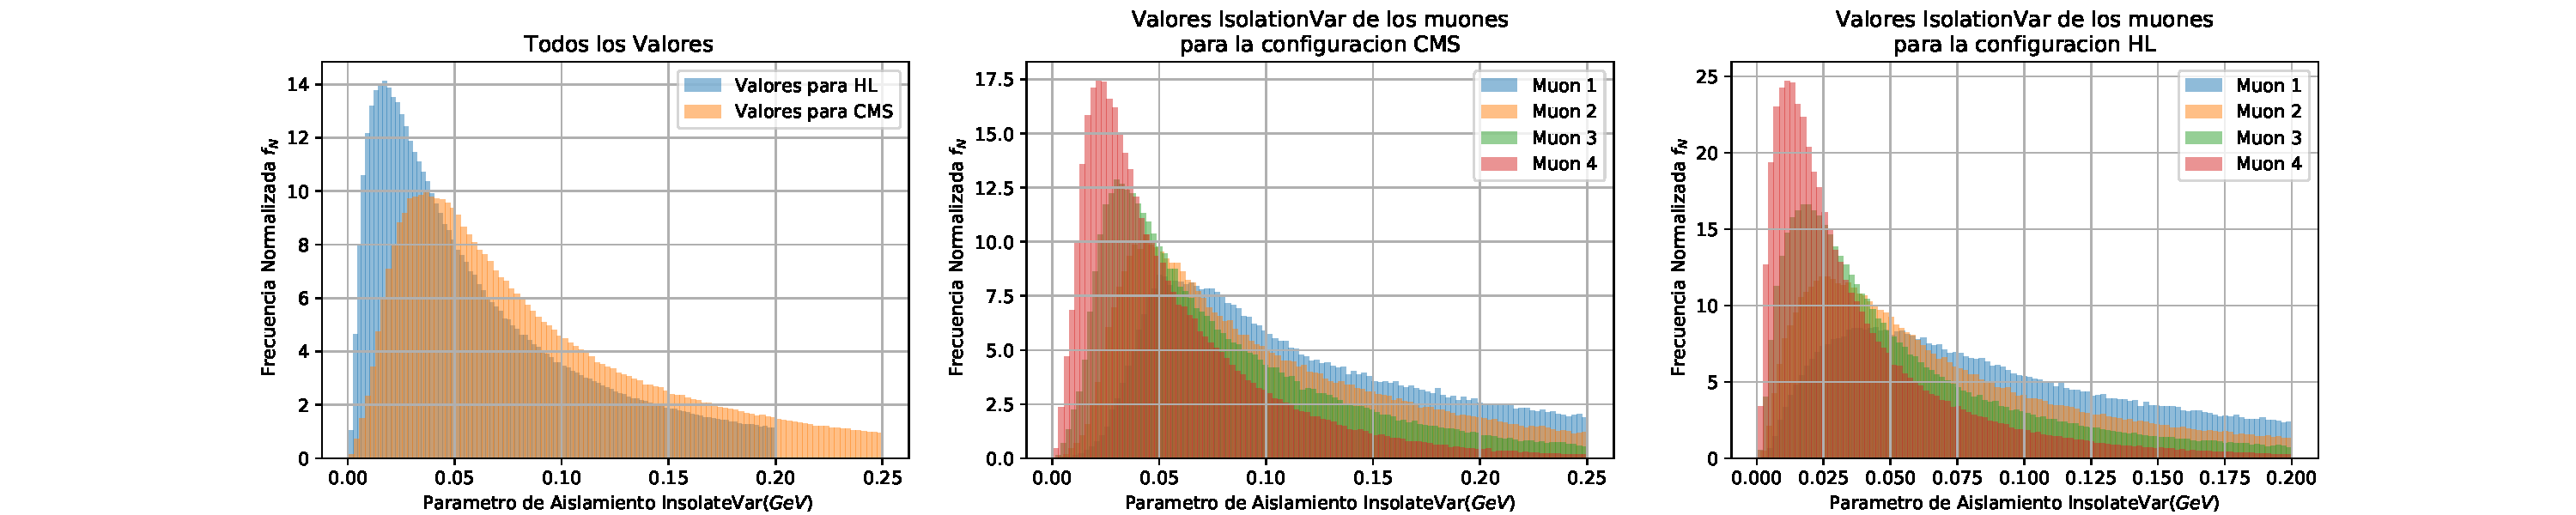
\includegraphics[width=.8\textwidth]{Simulacion/imagenes/Datos_IsolationVar_ALL.png}
\caption{Caracterización global de los momentos transversales de nuestra población de muones reconstruidos.}
\label{procesos_darksusy_PTyISO}
\end{figure}



\subsubsection{Valores de angulo}
\begin{figure}[!ht]
\centering
\includegraphics[width=.8\textwidth]{Simulacion/imagenes/Datos_Eta_ALL.png}
\includegraphics[width=.8\textwidth]{Simulacion/imagenes/Datos_Phi_ALL.png}
\caption{Grupo total de datos generados para los eventos de interes.}
\label{procesos_darksusy_ETAyPHI}
\end{figure}





Otro factor importante en la detección de los muones es el valor de Entonces de forma generar se puede Además como límite superior se puede constatar que el  se encuentran para valores 




















    
	\section{Reconstrucción de los fotones oscuros.}
	
		\subsection{Reconstrucción de los eventos con 4 muones.}
		


\begin{figure}[ht]
\centering
\includegraphics[width=1\textwidth]{Simulacion/imagenes/Datos_Photon4muon_ALL.png}
\caption{.}
\label{genera_darksusy}
\end{figure}





		
		\subsection{Reconstrucción de los eventos con menos de 4 muones.}	
		\begin{figure}[ht]
\centering
\includegraphics[width=1\textwidth]{Simulacion/imagenes/proceso_genera_darksusy2_.png}
\caption{Diagrama de flujo de programación para el análisis de los eventos con 3 y dos muones.}
\label{genera_darksusy}
\end{figure}
		
		\subsection{Reconstrucción total de fotones oscuros.}	
		 
\begin{figure}[h!]
    \centering
    \includegraphics[width=1\textwidth]{Simulacion/imagenes/Porciento_fotones_oscuros.png}
    \caption{Análisis del porciento de reconstrucción de lo fotones oscuros.}
    \label{}
\end{figure}


 
 
 
 

    
    \section{Aislamiento.}
    

    
    %\section{Muon efficiency parametrization}

%\section{Integration of Dark-SUSY model}

%\section{Delphes Simulation}

%\section{Muon system}

%\subsection{CMS detector}

%\subsection{Luminosity Era}

%\chapter{Simulation}

%\section{Parton Level and Hadronization}

%\section{Detector simulation}

%\chapter{Next steps}

%% Resultados y Analisis
%%\begin{textblock}{9}(2.5,-3)
%\begin{flushright}
%\setlength{\baselineskip}{15pt}
%\textblockrulecolour{white}
%~
%
%`` La discrepancia entre lo que se esperaba y lo que se ha observado ha aumentado a lo largo de los años, y nos estamos esforzando cada vez más por llenar el vacío
%''\\[.5cm]
%\textit{Jeremiah P. Ostriker}
%\end{flushright}
%\end{textblock}

En este capítulo se realiza una descripción del experimento \CMS, y una descripción del proceso de actualización de los detectores que lo componen. Se definen conceptos básicos correspondientes a la Física de Altas Energías experimental. Se introducen las herramientas personalizadas para el trabajo de simulación, análisis y caracterización en el área de partículas, entre estas se encuentras \ROOT, \textbf{Delphes}, \textbf{Pythia8} o \textbf{Madgraph}. Además, se introducen elementos comparativos para la caracterización del experimento en las configuración actual Run-2 y en la prevista en el futuro correspondiente a Alta Luminosidad.

%necesarios para el cumplimiento de los objetivos, estos serán descritos para su mejor comprensión en el proceso de simulación, caracterización y análisis de resultados. Además se resumirán los resultados que servirán de antecedentes para la investigación.






%\section{Algoritmo para el pareamiento de Muones}
Para la identificación de los procesos se implementa un algoritmo para la identificación de los decaimientos a dos muones y la identificacion de los di-muones en él:
\begin{figure}[ht!]
    \centering
    \includegraphics[width=0.84\textwidth]{Analisis_y_Resultados/imagenes/diagrama_pair.png}
    \caption{Diagrama de flujo para la identificación de los pares en los eventos a estudiar.}
    \label{fig:diagrama_pair}
\end{figure}


\section{Caracterizacion de la Señal}

%\begin{figure}[ht!]
%    \centering
    \includegraphics[width=0.84\textwidth]{Analisis_y_Resultados/imagenes/Cambio_de_D0_con_Card.png}
    
    \includegraphics[width=0.84\textwidth]{Analisis_y_Resultados/imagenes/Cambio_de_DZ_con_Card.png}
    
    \includegraphics[width=0.84\textwidth]{Analisis_y_Resultados/imagenes/Cambio_de_Eta_con_Card.png}
    
    \includegraphics[width=0.84\textwidth]{Analisis_y_Resultados/imagenes/Cambio_de_D0_con_Card.png}
    
    \includegraphics[width=0.84\textwidth]{Analisis_y_Resultados/imagenes/Cambio_de_IsolationVar_con_Card.png}
    
    \includegraphics[width=0.84\textwidth]{Analisis_y_Resultados/imagenes/Cambio_de_MassInv_con_Card.png}
    
    
    \includegraphics[width=0.84\textwidth]{Analisis_y_Resultados/imagenes/Cambio_de_Phi_con_Card.png}
    
    
    \includegraphics[width=0.84\textwidth]{Analisis_y_Resultados/imagenes/Cambio_de_PT_con_Card.png}
    
    





%\end{figure}




\begin{figure}[ht!]
    \centering
    \includegraphics[width=0.84\textwidth]{Analisis_y_Resultados/imagenes/evento_68.png}
    \caption{Representación esquematica de los pares generados en el evento 68 simulado: a) Reconstrucción con EVE; b) Identificación de elementos con C++.}
    \label{fig:diagrama_pair}
\end{figure}
\begin{figure}[ht!]
    \centering
    \includegraphics[width=0.84\textwidth]{Analisis_y_Resultados/imagenes/evento_68_info.png}
    \caption{Corte del informe del proceso de selección con C++ del evento 68.}
    \label{fig:diagrama_pair}
\end{figure}
\begin{figure}[ht!]
    \centering
    \includegraphics[width=0.84\textwidth]{Analisis_y_Resultados/imagenes/evento_7520.png}
    \caption{Representación esquematica de los pares generados en el evento 7520 simulado: a) Reconstrucción con EVE; b) Identificación de elementos con C++.}
    \label{fig:diagrama_pair}
\end{figure}
\begin{figure}[ht!]
    \centering
    \includegraphics[width=0.84\textwidth]{Analisis_y_Resultados/imagenes/evento_7520_info.png}
    \caption{Corte del informe del proceso de selección con C++ del evento 7520.}
    \label{fig:diagrama_pair}
\end{figure}

\begin{figure}[ht!]
    \centering
    \includegraphics[width=0.84\textwidth]{Analisis_y_Resultados/imagenes/mass.pdf}
    \caption{Masa invariante de los fotones pareados de nuestra se\~nal.}
    \label{fig:diagrama_pair}
\end{figure}

\begin{figure}[ht!]
    \centering
    \includegraphics[width=0.84\textwidth]{Analisis_y_Resultados/imagenes/MASS2.pdf}
    \caption{Masa invariante de los fotones pareados de nuestra se\~nal separados en los menores y los mayores.}
    \label{fig:diagrama_pair}
\end{figure}

\begin{figure}[ht!]
    \centering
    \includegraphics[width=0.84\textwidth]{Analisis_y_Resultados/imagenes/mulPT.pdf}
    \caption{Momento Angular ordenada para cada muon de nuestra se\~nal .}
    \label{fig:diagrama_pair}
\end{figure}



\section{Seleccion de Eventos}

La selecci\'on de eventos considera los cortes a distribuciones necesarios para maximizar la se\~nal y reducir lo mas posible la contribuci\'on 

\begin{table}[]
    \centering
    \begin{tabular}{|c|c|c|c|c|c|}
        \hline\hline
                                        & \multicolumn{5}{|c|}{N\'umero de Eventos HLLHC/CMS} \\

        Selecci\'on                     & c$\tau$=0mm   &  c$\tau$=5mm  & c$\tau$=10mm  & c$\tau$= 50mm & c$\tau$= 100mm\\ \hline
        Total                           & 10,000        & 10,000        & 10,000        & 10,000        & 10,000 \\ \hline
        (muones) $\mu >= 4$               & 1625 / 881    & 902/500       & 433/227       & 39/16         & 6/2 \\ \hline
        (di-muones)$\mu^+ \mu^->~= ~ 2$ & 1625 / 881    & 902/500       & 433/227       & 39/16         & 6/2 \\ \hline
        Isolation $<~ 2 GeV$            &               &               &               &               & \\ \hline\hline
    \end{tabular}
    \caption{Selecci\'on de eventos para muestras con masa de ``dark photon'' de $\gamma_{D}^{m}$ = 0.25 GeV}
    \label{tab:my_label}
\end{table}

%%%%%%%%%%%%%%%%%%%%%%%%%%
%% Anexos %%
%%%%%%%%%%%%%%%%%%%%%%%%%%
\chapter*{Anexo A}\label{anexoA}
Muchos fenónemos cosmólogicos han dado indicios de la existencia de materia oscura en sus diferentes composiciones teóricas, dado por lo cual un gran conjunto de experimentos han sido dedicados únicamente con la intención de obtener información pertinente en la comprensión de su composición y explicación de su comportamiento, existen dos métodos para realizar mediciones dimensionales:

% https://www.mpi-hd.mpg.de/hfm/CosmicRay/CosmicRaySites.html
\subsubsection{Forma directa}
Los métodos de detección directa intentan detectar las esporádicas interacciones que, a su paso por la Tierra, podrían experimentar
las partículas de materia oscura con un material adecuado y muy bien aislado del entorno.%Las mediciones directas utilizan instrumentos de medición para medir las propiedades físicas del objeto directamente, las mismas se pueden realizar en un amplio rango, especificado por la escala del instrumento de medición. 
Algunos experimentos de masa oscura son:

\begin{itemize_f}
\item[-] \href{https://en.wikipedia.org/wiki/Axion_Dark_Matter_Experiment}{ \textbf{ADMX} (\textbf{A}xion \textbf{D}ark \textbf{M}atter e\textbf{X}periment) :} 
\begin{itemize_f}
\item \textbf{Nombre:} \href{https://en.wikipedia.org/wiki/Axion_Dark_Matter_Experiment}{Experimento de Materia Oscura \Axion}
\item \textbf{Resumen:} Utiliza una cavidad de microondas resonante dentro de un gran imán superconductor para buscar \axiones~ de materia oscura fría en el halo local de materia oscura galáctica. 
\item \textbf{Pagina del proyecto :} \url{https://depts.washington.edu/admx/publications.shtml\#}
\end{itemize_f}




\item[-]\href{https://en.wikipedia.org/wiki/ANAIS}{\textbf{ANAIS} (\textbf{A}nnual modulation with \textbf{NAI} \textbf{S}cintillators) :} 
\begin{itemize_f}
\item \textbf{Nombre:} \href{https://en.wikipedia.org/wiki/ANAIS}{Modulación anual con NaI} \href{https://es.wikipedia.org/wiki/Centelleador}{Centelleador}.
\item \textbf{Resumen:} Busca la modulación anual de la señal con centelleadores de \href{https://es.wikipedia.org/wiki/Yoduro_de_sodio}{$NaI$} con el objetivo de detectar directamente  la Materia Oscura galáctica a través de su dispersión con los núcleos blanco de un cristal de NaI(Tl) radiopuro. Esta señal de Materia Oscura debería estar modulada anualmente debido al cambio de la velocidad relativa \WIMP-núcleo, consecuencia de la rotación de la Tierra alrededor del Sol.
\item \textbf{Pagina del proyecto :} \url{https://gifna.unizar.es/anais/}.
\end{itemize_f}

\item[-] \href{https://en.wikipedia.org/wiki/ArDM}{\textbf{ArDM} (\textbf{Ar}gon \textbf{D}ark \textbf{M}atter): }
\begin{itemize_f}
\item \textbf{Nombre:} \href{https://en.wikipedia.org/wiki/ArDM}{Materia Oscura en el Argón.}
\item \textbf{Resumen:} Busca medir y observando electrones libres de ionización y fotones de centelleo, que son producidos por la interación de su núcleo con los átomos vecinos y de esta forma relacionarla con la dispersión elástica de \WIMP ~ de los núcleos de argón líquido del que esta hecho el detector.
\item \textbf{Pagina del proyecto :} \url{https://wikimili.com/en/China_Jinping_Underground_Laboratory}.
\end{itemize_f}

%\item[-] \href{https://en.wikipedia.org/wiki/China_Dark_Matter_Experiment}{China Dark Matter Experiment (CDEX)}
%\begin{itemize_f}
%\item \textbf{Nombre:} 
%\item \textbf{Resumen:} 
%\item \textbf{Pagina del proyecto :} \url{}
%\end{itemize_f}

\item[-] \href{https://en.wikipedia.org/wiki/Cryogenic_Dark_Matter_Search}{\textbf{CDMS} (\textbf{C}ryogenic \textbf{D}ark \textbf{M}atter \textbf{S}earch)}
\begin{itemize_f}
\item \textbf{Nombre:} \href{https://en.wikipedia.org/wiki/Cryogenic_Dark_Matter_Search}{Buscando Materia Oscura Criogénica}
\item \textbf{Resumen:} Busca utilizando una serie de detectores de semiconductores a temperaturas de milikelvin encontrar los límites más sensibles en las interacciones de la materia oscura \WIMP~  con materiales terrestres y de esta manera detectar directamente la materia oscura. Constituye una serie de experimentos continuos: el \textbf{CDMS I}, \textbf{CDMS II}, el \textbf{SuperCDMS} y en la actualidad continúa con \textbf{SuperCDMS SNOLAB}.
\item \textbf{Pagina del proyecto :} \url{https://supercdms.slac.stanford.edu/}
\end{itemize_f}

%\item[-] \href{https://en.wikipedia.org/wiki/Cryogenic_Low-Energy_Astrophysics_with_Neon}{The Cryogenic Low-Energy Astrophysics with Noble liquids (CLEAN)}

%\item[-] \href{https://en.wikipedia.org/wiki/CoGeNT}{CoGeNT}
%\begin{itemize_f}
%\item \textbf{Nombre:} 
%\item \textbf{Resumen:} 
%\item \textbf{Pagina del proyecto :} \url{}
%\end{itemize_f}

%\item[-] \href{https://en.wikipedia.org/wiki/DAMA/LIBRA}{DAMA/LIBRA experiment}
%\begin{itemize_f}
%\item \textbf{Nombre:} Experimento \textbf{DAMA/LIBRA}
%\item \textbf{Resumen:} 
%\item \textbf{Pagina del proyecto :} \url{}
%\end{itemize_f}

\item[-] \href{https://en.wikipedia.org/wiki/DAMA/NaI}{DAMA/NaI experiment}
\begin{itemize_f}
\item \textbf{Nombre:} \href{https://en.wikipedia.org/wiki/DAMA/NaI}{Experimento DAMA/NaI}
\item \textbf{Resumen:} Características semejantes al experimento \href{https://en.wikipedia.org/wiki/ANAIS}{\textbf{ANAIS}} con mas de 7 años de datos de datos recopilados, fue continuado su estudio con el experimento \href{https://en.wikipedia.org/wiki/DAMA/LIBRA}{DAMA/LIBRA}.
\item \textbf{Pagina del proyecto :} \url{https://people.roma2.infn.it/~dama/web/home.html}
\end{itemize_f}

\item[-] \href{https://en.wikipedia.org/wiki/DarkSide}{DarkSide}
\begin{itemize_f}
\item \textbf{Nombre:} \href{https://en.wikipedia.org/wiki/DarkSide}{DarkSide}
\item \textbf{Resumen:} Busca con la construcción y operación de una serie de cámaras de proyección de tiempo o \href{https://en.wikipedia.org/wiki/Time_projection_chamber}{\textbf{TPC} (\textbf{T}ime \textbf{P}rojection \textbf{C}hamber)} de argón líquido para detectar \WIMPs. 
\item \textbf{Pagina del proyecto :} \url{http://darkside.lngs.infn.it/}
\end{itemize_f}

\item[-] \href{https://en.wikipedia.org/wiki/DEAP}{\textbf{DEAP} (\textbf{D}ark matter \textbf{E}xperiment using \textbf{A}rgon \textbf{P}ulse-shape discrimination)}
\begin{itemize_f}
\item \textbf{Nombre:} Experimento de materia oscura con discriminación de forma de pulso de argón
\item \textbf{Resumen:}) Busca discriminación de fondo basada en la característica forma de pulso de centelleo del argón permitiendo medir directamente \WIMP.
\item \textbf{Pagina del proyecto :} \url{http://deap3600.ca/}
\end{itemize_f}

%\item[-] \href{https://en.wikipedia.org/wiki/Monopole,_Astrophysics_and_Cosmic_Ray_Observatory}{MACRO (Monopole, Astrophysics and Cosmic Ray Observatory)}
%\begin{itemize_f}
%\item \textbf{Nombre:} 
%\item \textbf{Resumen:} 
%\item \textbf{Pagina del proyecto :} \url{}
%\end{itemize_f}
%
%\item[-] \href{https://en.wikipedia.org/wiki/PandaX}{PandaX (Particle and Astrophysical Xenon Detector)}
%\begin{itemize_f}
%\item \textbf{Nombre:} 
%\item \textbf{Resumen:} 
%\item \textbf{Pagina del proyecto :} \url{}
%\end{itemize_f}
%
%\item[-] \href{https://en.wikipedia.org/wiki/WIMP_Argon_Programme}{WIMP Argon Programme (WARP) }
%\begin{itemize_f}
%\item \textbf{Nombre:} 
%\item \textbf{Resumen:} 
%\item \textbf{Pagina del proyecto :} \url{}
%\end{itemize_f}
%
%\item[-] \href{https://en.wikipedia.org/wiki/XENON}{XENON}
%\begin{itemize_f}
%\item \textbf{Nombre:} 
%\item \textbf{Resumen:} 
%\item \textbf{Pagina del proyecto :} \url{}
%\end{itemize_f}
%
%\item[-] \href{https://en.wikipedia.org/wiki/ZEPLIN-III}{ZEPLIN-III dark matter experiment}
%\begin{itemize_f}
%\item \textbf{Nombre:} 
%\item \textbf{Resumen:} 
%\item \textbf{Pagina del proyecto :} \url{}
%\end{itemize_f}
%
%\item[-] \href{https://en.wikipedia.org/wiki/UK_Dark_Matter_Collaboration}{UK Dark Matter Collaboration (UKDMC)}
%\begin{itemize_f}
%\item \textbf{Nombre:} 
%\item \textbf{Resumen:} 
%\item \textbf{Pagina del proyecto :} \url{}
%\end{itemize_f}

\item[-] Otros experimentos : 
\begin{itemize_f}
\item \href{https://en.wikipedia.org/wiki/Monopole,_Astrophysics_and_Cosmic_Ray_Observatory}{\textbf{MACRO} (\textbf{M}onopole, \textbf{A}strophysics and \textbf{C}osmic \textbf{R}ay \textbf{O}bservatory)}, 

\textbf{Pagina del proyecto :} \url{https://hepwww.pp.rl.ac.uk/groups/ukdmc/ukdmc_old.html}

\item \href{https://en.wikipedia.org/wiki/PandaX}{PandaX (\textbf{P}article and Astrophysical \textbf{X}enon Detector)}, 

\textbf{Pagina del proyecto :} \url{https://pandax.sjtu.edu.cn/}

\item \href{https://en.wikipedia.org/wiki/WIMP_Argon_Programme}{\textbf{WARP} (\textbf{W}IMP \textbf{AR}gon \textbf{P}rogramme)}, 

\textbf{Pagina del proyecto :} \url{https://ztopics.com/WIMP\%20Argon\%20Programme/}

\item \href{https://en.wikipedia.org/wiki/XENON}{XENON}, 

\textbf{Pagina del proyecto :} \url{http://www.xenon1t.org/}

\item \href{https://en.wikipedia.org/wiki/ZEPLIN-III}{ZEPLIN-III dark matter experiment}, 

\textbf{Pagina del proyecto :} \url{https://zeplin.io/}

\item \href{https://en.wikipedia.org/wiki/UK_Dark_Matter_Collaboration}{\textbf{UKDMC} (\textbf{UK} \textbf{D}ark \textbf{M}atter \textbf{C}ollaboration)}, 

\textbf{Pagina del proyecto :} \url{https://hepwww.pp.rl.ac.uk/groups/ukdmc/ukdmc.html}
\end{itemize_f}
\end{itemize_f}


\subsubsection{Forma indirecta}
Otro mecanismo de investigación es cuando el valor de la propiedad física se obtiene a partir de lecturas directas de otras propiedades y de una expresión matemática que las relacione. Las medidas indirectas calculan el valor de la medida mediante una expresión matemática fundamentada por la teoría, previo cálculo de las magnitudes que intervienen en la expresión por medidas directas. Algunas investigaciones relacionadas con este mecanismo son: 

\begin{itemize_f}

\item[-] \href{https://en.wikipedia.org/wiki/Alpha_Magnetic_Spectrometer}{\textbf{AMS-02} (\textbf{A}lpha \textbf{M}agnetic \textbf{S}pectrometer)}
\begin{itemize_f}\label{AMS}
\item \textbf{Nombre:} Espectrómetro Magnético Alfa
\item \textbf{Resumen:} Busca con un detector localizado en Estación Espacial Internacional o \textbf{ISS} (\textbf{I}nternational \textbf{S}pace \textbf{S}tation) medir la antimateria en los rayos cósmicos, detectando picos en el flujo de positrones, antiprotones o rayos gamma pudiendo indicar la presencia de \neutralinos. El \textbf{AMS-01} es referido al prototipo de \textbf{AMS}, conteniendo este una versión simplificada del detector usado. Algunos de sus resultados se muestran en las referencias \cite{li_antiproton_2017,battiston_anti_2008}
\item \textbf{Pagina del proyecto :} \url{https://ams.nasa.gov/}
\end{itemize_f}

\item[-] \href{https://en.wikipedia.org/wiki/ANTARES_(telescope)}{\textbf{ANTARES} (\textbf{A}stronomy with a \textbf{N}eutrino \textbf{T}elescope and \textbf{A}byss environmental \textbf{RES}earch project)}
\begin{itemize_f}\label{antares}
\item \textbf{Nombre:} Astronomía con un Proyecto de Investigación Ambiental del Telescopio de Neutrinos y Abyss.
\item \textbf{Resumen:} Busca con sus tubos fotomultiplicadores detectar la radiación Cherenkov emitida cuando el muón pasa a través del agua, las técnicas de detección utilizadas consiguen en distinguir entre la señal de muones "que van hacia arriba", de neutrinos muónicos que interaccionan antes de llegar por debajo al detector y del alto flujo de muones procedentes de la atmósfera, con los datos y la alta resolución de estos pretende buscar indicaciones de materia oscura detectando el proceso de aniquilación del neutralino en el Sol. El proyecto \textbf{ANTARES} complementa el Observatorio de Neutrinos IceCube en la Antártida. Otros telescopios de neutrinos diseñados para su uso en el área cercana incluyen el telescopio griego \textbf{NESTOR} y el italiano \textbf{NEMO}. 

\item \textbf{Pagina del proyecto :} \url{https://antares.in2p3.fr/}

~~~~~~~~~~~~~~~~~~~~~~~~~~~~~~~~~\url{https://icecube.wisc.edu/}

~~~~~~~~~~~~~~~~~~~~~~~~~~~~~~~~~\url{https://cds.cern.ch/record/5841}

~~~~~~~~~~~~~~~~~~~~~~~~~~~~~~~~~\url{http://nemo.in2p3.fr/nemow3/index.html}
\end{itemize_f}

\item[-] \href{https://en.wikipedia.org/wiki/Calorimetric_Electron_Telescope}{\textbf{CALET} (\textbf{CAL}orimetric \textbf{E}lectron \textbf{T}elescope)}
\begin{itemize_f}\label{calet}
\item \textbf{Nombre:} Telescopio de electrones calorimétrico
\item \textbf{Resumen:} Busca realizar un seguimiento de la trayectoria de electrones, protones, núcleos y rayos gamma, mediante la medición de su dirección, carga y energía, para esto hace uso de un telescopio espacial de alta precisión.
\item \textbf{Pagina del proyecto :} \url{https://iss.jaxa.jp/en/kiboexp/ef/calet/}
\end{itemize_f}

%\item[-] \href{https://en.wikipedia.org/wiki/CERN_Axion_Solar_Telescope}{\textbf{CAST} (\textbf{C}ERN \textbf{A}xion \textbf{S}olar \textbf{T}elescope) }
%\begin{itemize_f}
%\item \textbf{Nombre:} 
%\item \textbf{Resumen:} es un experimento en física de astropartículas para buscar axiones que se originan en el sol. El experimento, realizado en el CERN en Suiza, comenzó en 2002 con la primera toma de datos a partir de mayo de 2003. La detección exitosa de los axiones solares constituiría un descubrimiento importante en la física de partículas y también abriría una nueva ventana sobre La astrofísica del núcleo solar.
%\item \textbf{Pagina del proyecto :} \url{}
%\end{itemize_f}

\item[-] \href{https://en.wikipedia.org/wiki/Dark_Matter_Particle_Explorer}{\textbf{DAMPE} (\textbf{DA}rk \textbf{M}atter \textbf{P}article \textbf{E}xplorer)}
\begin{itemize_f}
\item \textbf{Nombre:} Explorando Particulas de Materia Oscura
\item \textbf{Resumen:} Busca señal de descomposición indirecta de un hipotético candidato de materia oscura \WIMP~  mediante la detección rayos gamma de alta energía, electrones e iones de rayos cósmicos, para esto se hace uso de un telescopio espacial localizado en el satélite \textbf{CAS}.
\item \textbf{Pagina del proyecto :} \url{http://dpnc.unige.ch/dampe/}
\end{itemize_f}

\item[-] \href{https://en.wikipedia.org/wiki/Fermi_Gamma-ray_Space_Telescope}{\textbf{FGST} (\textbf{F}ermi \textbf{G}amma-ray \textbf{S}pace \textbf{T}elescope)}
\begin{itemize_f}\label{fermi}
\item \textbf{Nombre:} Telescopio Espacial de Area Grande de Rayos Gamma  
\item \textbf{Resumen:} Busca haciendo haciendo uso de un observatorio espacial muestras astronómicas de rayos gamma desde la órbita terrestre baja para para estudiar fenómenos astrofísicos y cosmológicos como núcleos galácticos activos, púlsares, otras fuentes de alta energía y materia oscura. Su instrumento principal es el Telescopio de Área Grande o \textbf{LAT} (\textbf{L}arge \textbf{A}rea \textbf{T}elescope), con el cual los astrónomos pretenden realizar un levantamiento de todo el cielo. %El proyecto es un experimento reconocido del CERN.
\item \textbf{Pagina del proyecto :} \url{https://glast.sites.stanford.edu/}
\end{itemize_f}

\item[-] \href{https://en.wikipedia.org/wiki/PAMELA_detector}{\textbf{PAMELA} (\textbf{P}ayload for \textbf{A}ntimatter \textbf{M}atter \textbf{E}xploration and \textbf{L}ight-nuclei \textbf{A}strophysics)}
\begin{itemize_f}\label{pamela}
\item \textbf{Nombre:} Exploración de la Materia-Antimateria y Astrofísica de los Núcleos de Luz.
\item \textbf{Resumen:} Busca estudiar y detectar rayos cósmicos, con un enfoque particular en su componente antimateria, en forma de positrones y antiprotones, además monitorea a largo plazo de la modulación solar de los rayos cósmicos, partículas energéticas del Sol, partículas de alta energía en la magnetosfera de la Tierra y electrones jovianos, con el objetivo de detectar evidencia de aniquilación de materia oscura.
\item \textbf{Pagina del proyecto :} \url{https://pamela.roma2.infn.it/}
\end{itemize_f}

\item[-] \href{https://stratocat.com.ar/fichas-e/1991/FSU-19910923.htm}{\textbf{MASS} (\textbf{M}atter \textbf{A}ntimatter \textbf{S}uperconducting \textbf{S}pectrometer)}
\begin{itemize_f}\label{mass}
\item \textbf{Nombre:} Espectrómetro Superconductor de Materia-Antimateria.
\item \textbf{Resumen:} Busca con la adaptación de la configuración básica de la Instalación de Imanes en Globo investigar partículas de alta energía usando un espectrómetro de imán superconductor, un dispositivo de tiempo de vuelo, un contador de gas cherenkov y un calorímetro de imagen de tubo streamer, de esta manera medir antiprotones en el rango de energías entre $4-20~GeV$ y positrones de aproximadamente $4-10~GeV$. Se utilizó la misma configuración del experimento \textbf{MASS-1} excepto por el sistema de seguimiento.

\item \textbf{Pagina del proyecto :} \url{https://stratocat.com.ar/fichas-e/1991/FSU-19910923.htm}
\end{itemize_f}

\item[-] \href{https://core.ac.uk/display/25103181}{\textbf{CAPRICE} (\textbf{C}osmic \textbf{A}nti\textbf{P}article \textbf{R}ing \textbf{I}maging \textbf{C}herenkov \textbf{E}xperiment)}
\begin{itemize_f}
\item \textbf{Nombre:} Experimento Cósmico de Imágenes de Anillo de Antipartículas de Cherenkov.
\item \textbf{Resumen:} Busca estudiar el flujo de rayos cósmicos sin demasiado fondo de partículas producidas atmosféricamente, esto es posible por el uso de un espectrómetro capaz de discriminar entre diferentes partículas. El proyecto se enfoca en estudiar los núcleos de antimateria, luz en los rayos cósmicos así como los muones en la atmósfera, específicamente mide el flujo de las antipartículas (antiprotones y positrones) por encima de aproximadamente $5~ GeV$ y relaciona los flujos con modelos que incluyen la producción exótica de antipartículas como partículas supersimétricas de materia oscura. %El flujo de muones se mide durante el descenso del globo a través de la atmósfera. Estas mediciones de flujo son importantes para los cálculos del flujo de neutrinos atmosféricos y, por lo tanto, para la interpretación de la anomalía del neutrino atmosférico.
\item \textbf{Pagina del proyecto :} \url{https://cds.cern.ch/record/5608}
\end{itemize_f}

\item[-] \href{https://ui.adsabs.harvard.edu/abs/1995psu..reptR....B/abstract}{\textbf{HEAT} (\textbf{H}igh-\textbf{E}nergy \textbf{A}ntimatter \textbf{T}elescope)}
\begin{itemize_f}
\item \textbf{Nombre:} Telescopio de Antimateria de Altas Energías
\item \textbf{Resumen:} Busca optimizadar la detección e identificación de electrones de rayos cósmicos y positrones a energías de aproximadamente $1~ GeV$ hasta $50~GeV$, mediante la implementación de un imán superconductor de dos bobinas y un hodoscopio de seguimiento de precisión, complementado con un sistema de tiempo de vuelo, un detector de radiación de transición y un contador de ducha electromagnético, de esta forma medir la diferencia en el tiempo entre la detección de una partícula ionizante en un tubo de deriva y un impulso generado por el disparador del experimento. Algunos de sus resultados se muestran en la referencia \cite{hooper_kaluza-klein_2004}.
\item \textbf{Pagina del proyecto :} \url{http://stratocat.com.ar/fichas-e/1994/FSU-19940503.htm}
\end{itemize_f}

\item[-] \href{https://en.wikipedia.org/wiki/Large_Hadron_Collider}{\textbf{LHC} (\textbf{L}arge \textbf{H}adron \textbf{C}ollider)}
\begin{itemize_f}\label{lhc}
\item \textbf{Nombre:} Gran Colisionador de Hadrones
\item \textbf{Resumen:} Ya que debido a que una partícula de materia oscura debería tener interacciones insignificantes con la materia visible normal, entonces estás interacciones pueden detectarse indirectamente como energía y momento faltantes que escapan de los detectores como resultado de las colisiones de haces de protones. Cualquier descubrimiento en las búsquedas de los colisionadores debe ser corroborado por resultados en los sectores de detección indirecta o directa en otros experimentos.
\item \textbf{Pagina del proyecto :} \href{https://home.cern/science/accelerators/large-hadron-collider}{\texttt{https://home.cern/science/accelerators/}}

~~~~~~~~~~~~~~~~~~~~~~~~~~~~~~~~~\href{https://home.cern/science/accelerators/large-hadron-collider}{ \texttt{large-hadron-collider}}. %aaaaaaaaaaaaaaa aaaaaaaaaaaaaaa \url{https://wikimili.com/en/China_Jinping_Underground_Laboratory}
\end{itemize_f}


\item[-] Otros experimentos : 
\begin{itemize_f}
\item[-] \href{https://en.wikipedia.org/wiki/Microlensing_Observations_in_Astrophysics}{\textbf{MOA} (\textbf{M}icrolensing \textbf{O}bservations in \textbf{A}strophysics) }

\textbf{Pagina del proyecto :} \url{http://www.tekapotourism.co.nz/info/mt_john.html}

\item[-] \href{https://en.wikipedia.org/wiki/VERITAS}{\textbf{VERITAS} (\textbf{V}ery \textbf{E}nergetic \textbf{R}adiation \textbf{I}maging \textbf{T}elescope \textbf{A}rray \textbf{S}ystem)}

\textbf{Pagina del proyecto :} \url{https://veritas.sao.arizona.edu/}
\end{itemize_f}


\end{itemize_f}

%\subsubsection{Generanción de materia oscura por coalición}






%\bibliographystyle{UNAMThesis}
%\bibliographystyle{abbrv}
%\bibliographystyle{APA}
\bibliographystyle{UNAMThesis} % estilo bibliografico
\bibliography{ParticleUnison}
\addcontentsline{toc}{chapter}{Referencias Bibliográficas}
\end{document}
